% Chapter 5: Conditional volatility: ARCH and GARCH
% Time Series Analysis -- Bachelor's programmes Economic Informatics and Economic Cybernetics, Bucharest University of Economic Studies
% GENERATED by latex/build_chapter5.py -- edit the generator, not this file.

\newcommand{\coursename}{Time Series Analysis}
% Preambul comun TSA -- Serii de timp / Time Series Analysis (Beamer, 16:9)
% Același design ca MFM și SFM (preluat din SFM, 5 octombrie 2026). Înainte de % Preambul comun TSA -- Serii de timp / Time Series Analysis (Beamer, 16:9)
% Același design ca MFM și SFM (preluat din SFM, 5 octombrie 2026). Înainte de % Preambul comun TSA -- Serii de timp / Time Series Analysis (Beamer, 16:9)
% Același design ca MFM și SFM (preluat din SFM, 5 octombrie 2026). Înainte de \input{../../latex/preamble} se definește
%   \newcommand{\coursename}{Time Series Analysis}      (EN)
%   \newcommand{\coursename}{Serii de timp}       (RO)  și  \def\tsalang{ro}
% Fișierele .tex se află în EN/Courses, EN/Seminars, RO/Cursuri, RO/Seminarii (două niveluri sub rădăcină).
% Deck-urile sînt generate de latex/build_chapterN.py / build_seminarN.py (vezi latex/tsa_build.py).

\documentclass[9pt, aspectratio=169, t]{beamer}
\providecommand{\coursename}{Time Series Analysis}

% Ensure content fits on slides
\setbeamersize{text margin left=8mm, text margin right=8mm}
% Smaller institute font (title page)
\setbeamerfont{institute}{size=\footnotesize}

%=============================================================================
% THEME AND STYLE CONFIGURATION
%=============================================================================
\usetheme{default}
% Using default theme for clean header/footer control

% Color Palette (matching Redispatch PDF)
\definecolor{MainBlue}{RGB}{26, 58, 110}
\definecolor{AccentBlue}{RGB}{26, 58, 110}
\definecolor{IDAred}{RGB}{205, 0, 0}
\definecolor{DarkGray}{RGB}{51, 51, 51}
\definecolor{MediumGray}{RGB}{128, 128, 128}
\definecolor{LightGray}{RGB}{248, 248, 248}
\definecolor{VeryLightGray}{RGB}{235, 235, 235}
\definecolor{KeynoteGray}{RGB}{218, 218, 218}
\definecolor{SectionGray}{RGB}{120, 120, 120}
\definecolor{FooterGray}{RGB}{100, 100, 100}
\definecolor{Crimson}{RGB}{220, 53, 69}
\definecolor{Forest}{RGB}{46, 125, 50}
\definecolor{Amber}{RGB}{181, 133, 63}
\definecolor{Orange}{RGB}{230, 126, 34}
\definecolor{Purple}{RGB}{142, 68, 173}

% Gradient background (exact Keynote 315° gradient: white to RGB 218,218,218)
\setbeamertemplate{background}{%
    \begin{tikzpicture}[remember picture, overlay]
        \shade[shading=axis, shading angle=315,
        top color=white, bottom color=KeynoteGray]
        (current page.south west) rectangle (current page.north east);
    \end{tikzpicture}%
}
% Fallback solid color for compatibility
\setbeamercolor{background canvas}{bg=}

\setbeamercolor{palette primary}{bg=MainBlue, fg=white}
\setbeamercolor{palette secondary}{bg=MainBlue!85, fg=white}
\setbeamercolor{palette tertiary}{bg=MainBlue!70, fg=white}
\setbeamercolor{structure}{fg=MainBlue}
\setbeamercolor{title}{fg=IDAred}
\setbeamercolor{frametitle}{fg=IDAred, bg=}
\setbeamercolor{block title}{bg=MainBlue, fg=white}
\setbeamercolor{block body}{bg=VeryLightGray, fg=DarkGray}
\setbeamercolor{block title alerted}{bg=Crimson, fg=white}
\setbeamercolor{block body alerted}{bg=Crimson!8, fg=DarkGray}
\setbeamercolor{block title example}{bg=Forest, fg=white}
\setbeamercolor{block body example}{bg=Forest!8, fg=DarkGray}
\setbeamercolor{item}{fg=MainBlue}

% Footer colors (override Madrid theme blue)
\setbeamercolor{author in head/foot}{fg=FooterGray, bg=}
\setbeamercolor{title in head/foot}{fg=FooterGray, bg=}
\setbeamercolor{date in head/foot}{fg=FooterGray, bg=}
\setbeamercolor{section in head/foot}{fg=FooterGray, bg=}
\setbeamercolor{subsection in head/foot}{fg=FooterGray, bg=}

% Bullet styles (apply everywhere including blocks)
\setbeamertemplate{itemize item}{\color{MainBlue}$\boxdot$}
\setbeamertemplate{itemize subitem}{\color{MainBlue}$\blacktriangleright$}
\setbeamertemplate{itemize subsubitem}{\color{MainBlue}\tiny$\bullet$}
\setbeamertemplate{itemize/enumerate body begin}{\normalsize}
\setbeamertemplate{itemize/enumerate subbody begin}{\normalsize}

% Item spacing - compact style
\setlength{\leftmargini}{10pt}       % Level 1: minimal indent
\setlength{\leftmarginii}{10pt}      % Level 2: minimal additional indent
% Compact list spacing (zero extra space before/after lists in blocks)
\makeatletter
\def\@listi{\leftmargin\leftmargini \topsep 0pt \parsep 0pt \itemsep 0pt}
\def\@listii{\leftmargin\leftmarginii \topsep 0pt \parsep 0pt \itemsep 0pt}
\makeatother

\setbeamertemplate{navigation symbols}{}

%=============================================================================
% CUSTOM HEADLINE
%=============================================================================
\setbeamertemplate{headline}{%
    \vskip10pt%
    \hbox to \paperwidth{%
        \hskip0.5cm%
        {\small\color{FooterGray}\renewcommand{\hyperlink}[2]{##2}\insertsectionhead}%
        \hfill%
        \textcolor{FooterGray}{\small\insertframenumber}%
        \hskip0.5cm%
    }%
    \vskip4pt%
    {\color{FooterGray}\hrule height 0.4pt}%
}

%=============================================================================
% CUSTOM FOOTER
%=============================================================================
\usepackage{fontawesome5}

\setbeamertemplate{footline}{%
    {\color{FooterGray}\hrule height 0.4pt}%
    \vskip4pt%
    \hbox to \paperwidth{%
        \hskip0.5cm%
        \textcolor{FooterGray}{\small\coursename}%
        \hfill%
        \raisebox{-0.1em}{%
            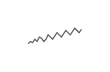
\begin{tikzpicture}[x=0.08em, y=0.08em, line width=0.4pt]
                \draw[FooterGray] (0,3) -- (1,4) -- (2,3.5) -- (3,5) -- (4,4) -- (5,6) -- (6,5.5) -- (7,4) -- (8,5) -- (9,7) -- (10,6) -- (11,5) -- (12,6.5) -- (13,8) -- (14,7) -- (15,6) -- (16,7.5) -- (17,9) -- (18,8) -- (19,7) -- (20,8.5) -- (21,10) -- (22,9) -- (23,8) -- (24,9.5);
            \end{tikzpicture}%
        }%
        \hskip0.5cm%
    }%
    \vskip6pt%
}

%=============================================================================
% PACKAGES
%=============================================================================
\usepackage[utf8]{inputenc}
\DeclareUnicodeCharacter{03B1}{\ensuremath{\alpha}}
\usepackage[T1]{fontenc}
\usepackage{amsmath, amssymb, amsthm}
\usepackage{mathtools}
\usepackage{bm}
\usepackage{tikz}
\usetikzlibrary{arrows.meta, positioning, shapes, calc, decorations.pathreplacing, shadings}
\usepackage{booktabs}
\usepackage{multirow}
\usepackage{array}
\usepackage{graphicx}
\usepackage{animate}
\usepackage{hyperref}
\usepackage{colortbl}
\usepackage{listings}
\lstset{language=Python, basicstyle=\ttfamily\scriptsize, keywordstyle=\color{MainBlue}\bfseries,
  commentstyle=\color{Forest}, stringstyle=\color{Crimson}, breaklines=true,
  frame=none, backgroundcolor=\color{VeryLightGray}, xleftmargin=2mm}
\hypersetup{colorlinks=true, linkcolor=MainBlue, urlcolor=MainBlue}
\graphicspath{{../../logos/}{../../charts/}{../../photos/}}
\usepackage{xcolor}
\hfuzz=2pt  % Suppress tiny overfull warnings (<2pt)
\vfuzz=2pt  % Suppress tiny vertical overfull warnings (<2pt)
% \mathrm in the sans-serif family of the slides (beamer resets \mathrm to the serif family at \begin{document};
% this hook runs after beamer's, so WN, Var, RMSE, ... in formulas match the surrounding text)
% Bold vectors and matrices in the same sans-serif family: \mathbf{A} in sans bold (beamer's own \mathbf came out in
% medium weight), and the bold upright Greek capitals of \boldsymbol / \bm (\bSigma, \bPhi, \boldsymbol{\Theta}) in
% cmss bold: bm.sty fixes its "boldoperators" font when it is loaded (serif cmbx), before beamer switches the
% operators to cmss, so it is reset here.
\AtBeginDocument{%
  \SetMathAlphabet{\mathrm}{normal}{\encodingdefault}{\sfdefault}{\mddefault}{n}%
  \SetMathAlphabet{\mathrm}{bold}{\encodingdefault}{\sfdefault}{bx}{n}%
  \SetMathAlphabet{\mathbf}{normal}{\encodingdefault}{\sfdefault}{bx}{n}%
  \SetMathAlphabet{\mathbf}{bold}{\encodingdefault}{\sfdefault}{bx}{n}%
  \SetSymbolFont{boldoperators}{normal}{OT1}{cmss}{bx}{n}%
  \SetSymbolFont{boldoperators}{bold}{OT1}{cmss}{bx}{n}}

%=============================================================================
% QUANTLET COMMANDS
%   \quantlet{<displayed name>}{<url>}       (generic, compatible with the older TSA decks)
%   \tsaquantlet{Ch_05}{TSA_ch5_garch}       -> https://github.com/danpele/Time-Series-Analysis/tree/main/Quantlets/Ch_05/TSA_ch5_garch
%   \qlurl{<folder>} is defined per chapter by the generator (Quantlets/Ch_NN/<folder>)
%=============================================================================
\newcommand{\tsarepo}{https://github.com/danpele/Time-Series-Analysis}
\newcommand{\tsaqlbase}{https://github.com/danpele/Time-Series-Analysis/tree/main/Quantlets}
\newcommand{\quantlet}[2]{%
    \hfill\href{#2}{%
        \raisebox{-0.15em}{
\includegraphics[height=0.7em]{ql_logo.png}}%
        \textcolor{MainBlue}{\tiny\ #1}%
    }%
}
\newcommand{\tsaquantlet}[2]{\quantlet{\detokenize{#2}}{\tsaqlbase/#1/#2}}

%=============================================================================
% NOTEBOOKS (Google Colab)
%   \colaburl{notebooks/EN/chapter5_seminar_notebook.ipynb} -> the Colab link of a file in the TSA repo
%   \nb: the chapter notebook (each seminar deck redefines it with \renewcommand)
%=============================================================================
\newcommand{\colaburl}[1]{https://colab.research.google.com/github/danpele/Time-Series-Analysis/blob/main/#1}
\newcommand{\nb}{https://colab.research.google.com/github/danpele/Time-Series-Analysis/tree/main/notebooks/EN}
\newcommand{\nbname}{notebooks/EN}

%=============================================================================
% SLIDE HELPERS (used by the generators; the same as in MFM)
%=============================================================================
% local font size for list bodies (the preamble forces \normalsize)
\newcommand{\itemsize}[1]{\setbeamertemplate{itemize/enumerate body begin}{#1}\setbeamertemplate{itemize/enumerate subbody begin}{#1}}
\newcommand{\intitle}[1]{{\hypersetup{urlcolor=white}#1}}   % white links inside coloured title bars
\newcommand{\imgcap}[1]{{\scriptsize #1}\\[0.5mm]}          % caption under a photo
\newcommand{\imgcredit}[2]{{\tiny\color{FooterGray}\href{#1}{#2}}}   % image credit: source URL, author/licence
\newcommand{\aiprompt}[1]{{\ttfamily\color{MainBlue}#1}}     % a prompt to an AI assistant

%=============================================================================
% SEMINARS: student version by default; the instructor wrapper *_solutions.tex sets \solutionstrue
%=============================================================================
\makeatletter\@ifundefined{ifsolutions}{\expandafter\newif\csname ifsolutions\endcsname}{}\makeatother
\newcommand{\solonly}[1]{\ifsolutions #1\fi}
\newcommand{\propsub}{\ifsolutions\else\framesubtitle{\ifdefined\tsalang Rezolvarea se discută la seminar\else Solution discussed in class\fi}\fi}

%=============================================================================
% APPENDIX AND CHAPTER LINKS (latex/appendix_links.py writes the calls; it also re-declares these
% macros before \begin{document}, so the decks compile with or without this preamble block)
%=============================================================================
\providecommand{\tsaapplink}[3]{\hypertarget{#2}{}\hyperlink{#1}{\beamergotobutton{#3}}}
\providecommand{\tsaappback}[2]{\begin{tikzpicture}[remember picture,overlay]\node[anchor=south east] at ([xshift=-3mm,yshift=7mm]current page.south east){\hyperlink{#1}{\beamerreturnbutton{#2}}};\end{tikzpicture}}
\providecommand{\tsachlink}[2]{\href{#1}{#2}}
\providecommand{\tsachlinkt}[2]{\href{#1}{\usebeamercolor[fg]{frametitle}#2}}

%=============================================================================
% QUANTINAR COMMAND: link către un curs Quantinar (subiecte avansate)
%=============================================================================
\newcommand{\quantinar}[2]{%
    \href{#2}{%
        \raisebox{-0.15em}{
\includegraphics[height=0.8em]{qr_logo.png}}%
        \textcolor{MainBlue}{\scriptsize\ #1}%
    }%
}

%=============================================================================
% CUSTOM TITLE PAGE
%=============================================================================
\defbeamertemplate*{title page}{hybrid}[1][]
{
    \vspace{0.2cm}
    % Logos row - top header (with clickable links)
    \begin{center}
        \href{https://www.ase.ro}{
\includegraphics[height=1.0cm]{ase_logo.png}}\hspace{0.3cm}%
        \href{https://theida.net}{
\includegraphics[height=1.0cm]{ida_logo.png}}\hspace{0.3cm}%
        \href{https://blockchain-research-center.com}{
\includegraphics[height=1.0cm]{brc_logo.png}}\hspace{0.3cm}%
        \href{https://www.ai4efin.ase.ro}{
\includegraphics[height=1.0cm]{ai4efin_logo.png}}\hspace{0.3cm}%
        \href{https://ipe.ro/new}{
\includegraphics[height=1.0cm]{acad_logo.png}}\hspace{0.3cm}%
        \href{https://www.digital-finance-msca.com}{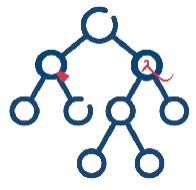
\includegraphics[height=1.0cm]{msca_logo.png}}%
    \end{center}

    \vspace{0.6cm}

    % Main title with Q logos on sides (with clickable links)
    \begin{center}
        \begin{minipage}{0.1\textwidth}
            \centering
            \href{https://quantlet.com}{
\includegraphics[height=1.1cm]{ql_logo.png}}
        \end{minipage}%
        \begin{minipage}{0.78\textwidth}
            \centering
            {\LARGE\bfseries\usebeamercolor[fg]{title}\inserttitle}

            \vspace{0.3cm}

            {\usebeamerfont{subtitle}\usebeamercolor[fg]{title}\insertsubtitle}
        \end{minipage}%
        \begin{minipage}{0.1\textwidth}
            \centering
            \href{https://quantinar.com}{
\includegraphics[height=1.1cm]{qr_logo.png}}
        \end{minipage}
    \end{center}

    \vspace{0.6cm}

    % Authors (left aligned)
    \hspace{0.5cm}{\usebeamerfont{author}\insertauthor}

    \vspace{0.3cm}

    % Institute/Affiliations (left aligned)
    \hspace{0.5cm}\begin{minipage}[t]{0.9\textwidth}
        \raggedright\small\insertinstitute
    \end{minipage}
}

%=============================================================================
% THEOREM ENVIRONMENTS
%=============================================================================
\theoremstyle{definition}
\setbeamertemplate{theorems}[numbered]
\ifdefined\tsalang
\newtheorem{defn}{Definiție}
\newtheorem{thm}{Teoremă}
\newtheorem{prop}{Propoziție}
\newtheorem{rmk}{Observație}
\else
\newtheorem{defn}{Definition}
\newtheorem{thm}{Theorem}
\newtheorem{prop}{Proposition}
\newtheorem{rmk}{Remark}
\fi

%=============================================================================
% CENTRED MINIPAGE (no extra vertical space)
%=============================================================================
\newenvironment{cminipage}[1]{%
    \par\noindent\hfill\begin{minipage}{#1}\ignorespaces
}{%
    \end{minipage}\hfill\null\par
}

%=============================================================================
% CUSTOM COMMANDS
%=============================================================================
\newcommand{\E}{\mathbb{E}}
\newcommand{\Var}{\text{Var}}
\newcommand{\Cov}{\text{Cov}}
\newcommand{\Corr}{\text{Corr}}
\newcommand{\R}{\mathbb{R}}
\newcommand{\N}{\mathbb{N}}
\newcommand{\Z}{\mathbb{Z}}
\newcommand{\B}{\mathbf{B}}
\newcommand{\imark}{\textcolor{MainBlue}{\textbullet}}
\newcommand{\RMSE}{\text{RMSE}}
\newcommand{\MAE}{\text{MAE}}
\newcommand{\MAPE}{\text{MAPE}}

% Boldface vector/matrix commands (VAR, VECM, state space; also used by the older TSA decks)
\newcommand{\bY}{\mathbf{Y}}
\newcommand{\bX}{\mathbf{X}}
\newcommand{\bA}{\mathbf{A}}
\newcommand{\bB}{\mathbf{B}}
\newcommand{\bepsilon}{\boldsymbol{\varepsilon}}
\newcommand{\bSigma}{\boldsymbol{\Sigma}}
\newcommand{\bPhi}{\boldsymbol{\Phi}}
\newcommand{\bGamma}{\boldsymbol{\Gamma}}
\newcommand{\bPi}{\boldsymbol{\Pi}}
\newcommand{\bc}{\mathbf{c}}
\newcommand{\balpha}{\boldsymbol{\alpha}}
\newcommand{\bbeta}{\boldsymbol{\beta}}
\newcommand{\bvarepsilon}{\boldsymbol{\varepsilon}}

% Legacy seminar marks (older TSA seminar decks)
\newcommand{\correct}{\textcolor{Forest}{\checkmark}}
\newcommand{\incorrect}{\textcolor{Crimson}{\texttimes}}
 se definește
%   \newcommand{\coursename}{Time Series Analysis}      (EN)
%   \newcommand{\coursename}{Serii de timp}       (RO)  și  \def\tsalang{ro}
% Fișierele .tex se află în EN/Courses, EN/Seminars, RO/Cursuri, RO/Seminarii (două niveluri sub rădăcină).
% Deck-urile sînt generate de latex/build_chapterN.py / build_seminarN.py (vezi latex/tsa_build.py).

\documentclass[9pt, aspectratio=169, t]{beamer}
\providecommand{\coursename}{Time Series Analysis}

% Ensure content fits on slides
\setbeamersize{text margin left=8mm, text margin right=8mm}
% Smaller institute font (title page)
\setbeamerfont{institute}{size=\footnotesize}

%=============================================================================
% THEME AND STYLE CONFIGURATION
%=============================================================================
\usetheme{default}
% Using default theme for clean header/footer control

% Color Palette (matching Redispatch PDF)
\definecolor{MainBlue}{RGB}{26, 58, 110}
\definecolor{AccentBlue}{RGB}{26, 58, 110}
\definecolor{IDAred}{RGB}{205, 0, 0}
\definecolor{DarkGray}{RGB}{51, 51, 51}
\definecolor{MediumGray}{RGB}{128, 128, 128}
\definecolor{LightGray}{RGB}{248, 248, 248}
\definecolor{VeryLightGray}{RGB}{235, 235, 235}
\definecolor{KeynoteGray}{RGB}{218, 218, 218}
\definecolor{SectionGray}{RGB}{120, 120, 120}
\definecolor{FooterGray}{RGB}{100, 100, 100}
\definecolor{Crimson}{RGB}{220, 53, 69}
\definecolor{Forest}{RGB}{46, 125, 50}
\definecolor{Amber}{RGB}{181, 133, 63}
\definecolor{Orange}{RGB}{230, 126, 34}
\definecolor{Purple}{RGB}{142, 68, 173}

% Gradient background (exact Keynote 315° gradient: white to RGB 218,218,218)
\setbeamertemplate{background}{%
    \begin{tikzpicture}[remember picture, overlay]
        \shade[shading=axis, shading angle=315,
        top color=white, bottom color=KeynoteGray]
        (current page.south west) rectangle (current page.north east);
    \end{tikzpicture}%
}
% Fallback solid color for compatibility
\setbeamercolor{background canvas}{bg=}

\setbeamercolor{palette primary}{bg=MainBlue, fg=white}
\setbeamercolor{palette secondary}{bg=MainBlue!85, fg=white}
\setbeamercolor{palette tertiary}{bg=MainBlue!70, fg=white}
\setbeamercolor{structure}{fg=MainBlue}
\setbeamercolor{title}{fg=IDAred}
\setbeamercolor{frametitle}{fg=IDAred, bg=}
\setbeamercolor{block title}{bg=MainBlue, fg=white}
\setbeamercolor{block body}{bg=VeryLightGray, fg=DarkGray}
\setbeamercolor{block title alerted}{bg=Crimson, fg=white}
\setbeamercolor{block body alerted}{bg=Crimson!8, fg=DarkGray}
\setbeamercolor{block title example}{bg=Forest, fg=white}
\setbeamercolor{block body example}{bg=Forest!8, fg=DarkGray}
\setbeamercolor{item}{fg=MainBlue}

% Footer colors (override Madrid theme blue)
\setbeamercolor{author in head/foot}{fg=FooterGray, bg=}
\setbeamercolor{title in head/foot}{fg=FooterGray, bg=}
\setbeamercolor{date in head/foot}{fg=FooterGray, bg=}
\setbeamercolor{section in head/foot}{fg=FooterGray, bg=}
\setbeamercolor{subsection in head/foot}{fg=FooterGray, bg=}

% Bullet styles (apply everywhere including blocks)
\setbeamertemplate{itemize item}{\color{MainBlue}$\boxdot$}
\setbeamertemplate{itemize subitem}{\color{MainBlue}$\blacktriangleright$}
\setbeamertemplate{itemize subsubitem}{\color{MainBlue}\tiny$\bullet$}
\setbeamertemplate{itemize/enumerate body begin}{\normalsize}
\setbeamertemplate{itemize/enumerate subbody begin}{\normalsize}

% Item spacing - compact style
\setlength{\leftmargini}{10pt}       % Level 1: minimal indent
\setlength{\leftmarginii}{10pt}      % Level 2: minimal additional indent
% Compact list spacing (zero extra space before/after lists in blocks)
\makeatletter
\def\@listi{\leftmargin\leftmargini \topsep 0pt \parsep 0pt \itemsep 0pt}
\def\@listii{\leftmargin\leftmarginii \topsep 0pt \parsep 0pt \itemsep 0pt}
\makeatother

\setbeamertemplate{navigation symbols}{}

%=============================================================================
% CUSTOM HEADLINE
%=============================================================================
\setbeamertemplate{headline}{%
    \vskip10pt%
    \hbox to \paperwidth{%
        \hskip0.5cm%
        {\small\color{FooterGray}\renewcommand{\hyperlink}[2]{##2}\insertsectionhead}%
        \hfill%
        \textcolor{FooterGray}{\small\insertframenumber}%
        \hskip0.5cm%
    }%
    \vskip4pt%
    {\color{FooterGray}\hrule height 0.4pt}%
}

%=============================================================================
% CUSTOM FOOTER
%=============================================================================
\usepackage{fontawesome5}

\setbeamertemplate{footline}{%
    {\color{FooterGray}\hrule height 0.4pt}%
    \vskip4pt%
    \hbox to \paperwidth{%
        \hskip0.5cm%
        \textcolor{FooterGray}{\small\coursename}%
        \hfill%
        \raisebox{-0.1em}{%
            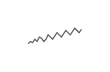
\begin{tikzpicture}[x=0.08em, y=0.08em, line width=0.4pt]
                \draw[FooterGray] (0,3) -- (1,4) -- (2,3.5) -- (3,5) -- (4,4) -- (5,6) -- (6,5.5) -- (7,4) -- (8,5) -- (9,7) -- (10,6) -- (11,5) -- (12,6.5) -- (13,8) -- (14,7) -- (15,6) -- (16,7.5) -- (17,9) -- (18,8) -- (19,7) -- (20,8.5) -- (21,10) -- (22,9) -- (23,8) -- (24,9.5);
            \end{tikzpicture}%
        }%
        \hskip0.5cm%
    }%
    \vskip6pt%
}

%=============================================================================
% PACKAGES
%=============================================================================
\usepackage[utf8]{inputenc}
\DeclareUnicodeCharacter{03B1}{\ensuremath{\alpha}}
\usepackage[T1]{fontenc}
\usepackage{amsmath, amssymb, amsthm}
\usepackage{mathtools}
\usepackage{bm}
\usepackage{tikz}
\usetikzlibrary{arrows.meta, positioning, shapes, calc, decorations.pathreplacing, shadings}
\usepackage{booktabs}
\usepackage{multirow}
\usepackage{array}
\usepackage{graphicx}
\usepackage{animate}
\usepackage{hyperref}
\usepackage{colortbl}
\usepackage{listings}
\lstset{language=Python, basicstyle=\ttfamily\scriptsize, keywordstyle=\color{MainBlue}\bfseries,
  commentstyle=\color{Forest}, stringstyle=\color{Crimson}, breaklines=true,
  frame=none, backgroundcolor=\color{VeryLightGray}, xleftmargin=2mm}
\hypersetup{colorlinks=true, linkcolor=MainBlue, urlcolor=MainBlue}
\graphicspath{{../../logos/}{../../charts/}{../../photos/}}
\usepackage{xcolor}
\hfuzz=2pt  % Suppress tiny overfull warnings (<2pt)
\vfuzz=2pt  % Suppress tiny vertical overfull warnings (<2pt)
% \mathrm in the sans-serif family of the slides (beamer resets \mathrm to the serif family at \begin{document};
% this hook runs after beamer's, so WN, Var, RMSE, ... in formulas match the surrounding text)
% Bold vectors and matrices in the same sans-serif family: \mathbf{A} in sans bold (beamer's own \mathbf came out in
% medium weight), and the bold upright Greek capitals of \boldsymbol / \bm (\bSigma, \bPhi, \boldsymbol{\Theta}) in
% cmss bold: bm.sty fixes its "boldoperators" font when it is loaded (serif cmbx), before beamer switches the
% operators to cmss, so it is reset here.
\AtBeginDocument{%
  \SetMathAlphabet{\mathrm}{normal}{\encodingdefault}{\sfdefault}{\mddefault}{n}%
  \SetMathAlphabet{\mathrm}{bold}{\encodingdefault}{\sfdefault}{bx}{n}%
  \SetMathAlphabet{\mathbf}{normal}{\encodingdefault}{\sfdefault}{bx}{n}%
  \SetMathAlphabet{\mathbf}{bold}{\encodingdefault}{\sfdefault}{bx}{n}%
  \SetSymbolFont{boldoperators}{normal}{OT1}{cmss}{bx}{n}%
  \SetSymbolFont{boldoperators}{bold}{OT1}{cmss}{bx}{n}}

%=============================================================================
% QUANTLET COMMANDS
%   \quantlet{<displayed name>}{<url>}       (generic, compatible with the older TSA decks)
%   \tsaquantlet{Ch_05}{TSA_ch5_garch}       -> https://github.com/danpele/Time-Series-Analysis/tree/main/Quantlets/Ch_05/TSA_ch5_garch
%   \qlurl{<folder>} is defined per chapter by the generator (Quantlets/Ch_NN/<folder>)
%=============================================================================
\newcommand{\tsarepo}{https://github.com/danpele/Time-Series-Analysis}
\newcommand{\tsaqlbase}{https://github.com/danpele/Time-Series-Analysis/tree/main/Quantlets}
\newcommand{\quantlet}[2]{%
    \hfill\href{#2}{%
        \raisebox{-0.15em}{
\includegraphics[height=0.7em]{ql_logo.png}}%
        \textcolor{MainBlue}{\tiny\ #1}%
    }%
}
\newcommand{\tsaquantlet}[2]{\quantlet{\detokenize{#2}}{\tsaqlbase/#1/#2}}

%=============================================================================
% NOTEBOOKS (Google Colab)
%   \colaburl{notebooks/EN/chapter5_seminar_notebook.ipynb} -> the Colab link of a file in the TSA repo
%   \nb: the chapter notebook (each seminar deck redefines it with \renewcommand)
%=============================================================================
\newcommand{\colaburl}[1]{https://colab.research.google.com/github/danpele/Time-Series-Analysis/blob/main/#1}
\newcommand{\nb}{https://colab.research.google.com/github/danpele/Time-Series-Analysis/tree/main/notebooks/EN}
\newcommand{\nbname}{notebooks/EN}

%=============================================================================
% SLIDE HELPERS (used by the generators; the same as in MFM)
%=============================================================================
% local font size for list bodies (the preamble forces \normalsize)
\newcommand{\itemsize}[1]{\setbeamertemplate{itemize/enumerate body begin}{#1}\setbeamertemplate{itemize/enumerate subbody begin}{#1}}
\newcommand{\intitle}[1]{{\hypersetup{urlcolor=white}#1}}   % white links inside coloured title bars
\newcommand{\imgcap}[1]{{\scriptsize #1}\\[0.5mm]}          % caption under a photo
\newcommand{\imgcredit}[2]{{\tiny\color{FooterGray}\href{#1}{#2}}}   % image credit: source URL, author/licence
\newcommand{\aiprompt}[1]{{\ttfamily\color{MainBlue}#1}}     % a prompt to an AI assistant

%=============================================================================
% SEMINARS: student version by default; the instructor wrapper *_solutions.tex sets \solutionstrue
%=============================================================================
\makeatletter\@ifundefined{ifsolutions}{\expandafter\newif\csname ifsolutions\endcsname}{}\makeatother
\newcommand{\solonly}[1]{\ifsolutions #1\fi}
\newcommand{\propsub}{\ifsolutions\else\framesubtitle{\ifdefined\tsalang Rezolvarea se discută la seminar\else Solution discussed in class\fi}\fi}

%=============================================================================
% APPENDIX AND CHAPTER LINKS (latex/appendix_links.py writes the calls; it also re-declares these
% macros before \begin{document}, so the decks compile with or without this preamble block)
%=============================================================================
\providecommand{\tsaapplink}[3]{\hypertarget{#2}{}\hyperlink{#1}{\beamergotobutton{#3}}}
\providecommand{\tsaappback}[2]{\begin{tikzpicture}[remember picture,overlay]\node[anchor=south east] at ([xshift=-3mm,yshift=7mm]current page.south east){\hyperlink{#1}{\beamerreturnbutton{#2}}};\end{tikzpicture}}
\providecommand{\tsachlink}[2]{\href{#1}{#2}}
\providecommand{\tsachlinkt}[2]{\href{#1}{\usebeamercolor[fg]{frametitle}#2}}

%=============================================================================
% QUANTINAR COMMAND: link către un curs Quantinar (subiecte avansate)
%=============================================================================
\newcommand{\quantinar}[2]{%
    \href{#2}{%
        \raisebox{-0.15em}{
\includegraphics[height=0.8em]{qr_logo.png}}%
        \textcolor{MainBlue}{\scriptsize\ #1}%
    }%
}

%=============================================================================
% CUSTOM TITLE PAGE
%=============================================================================
\defbeamertemplate*{title page}{hybrid}[1][]
{
    \vspace{0.2cm}
    % Logos row - top header (with clickable links)
    \begin{center}
        \href{https://www.ase.ro}{
\includegraphics[height=1.0cm]{ase_logo.png}}\hspace{0.3cm}%
        \href{https://theida.net}{
\includegraphics[height=1.0cm]{ida_logo.png}}\hspace{0.3cm}%
        \href{https://blockchain-research-center.com}{
\includegraphics[height=1.0cm]{brc_logo.png}}\hspace{0.3cm}%
        \href{https://www.ai4efin.ase.ro}{
\includegraphics[height=1.0cm]{ai4efin_logo.png}}\hspace{0.3cm}%
        \href{https://ipe.ro/new}{
\includegraphics[height=1.0cm]{acad_logo.png}}\hspace{0.3cm}%
        \href{https://www.digital-finance-msca.com}{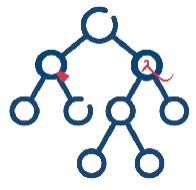
\includegraphics[height=1.0cm]{msca_logo.png}}%
    \end{center}

    \vspace{0.6cm}

    % Main title with Q logos on sides (with clickable links)
    \begin{center}
        \begin{minipage}{0.1\textwidth}
            \centering
            \href{https://quantlet.com}{
\includegraphics[height=1.1cm]{ql_logo.png}}
        \end{minipage}%
        \begin{minipage}{0.78\textwidth}
            \centering
            {\LARGE\bfseries\usebeamercolor[fg]{title}\inserttitle}

            \vspace{0.3cm}

            {\usebeamerfont{subtitle}\usebeamercolor[fg]{title}\insertsubtitle}
        \end{minipage}%
        \begin{minipage}{0.1\textwidth}
            \centering
            \href{https://quantinar.com}{
\includegraphics[height=1.1cm]{qr_logo.png}}
        \end{minipage}
    \end{center}

    \vspace{0.6cm}

    % Authors (left aligned)
    \hspace{0.5cm}{\usebeamerfont{author}\insertauthor}

    \vspace{0.3cm}

    % Institute/Affiliations (left aligned)
    \hspace{0.5cm}\begin{minipage}[t]{0.9\textwidth}
        \raggedright\small\insertinstitute
    \end{minipage}
}

%=============================================================================
% THEOREM ENVIRONMENTS
%=============================================================================
\theoremstyle{definition}
\setbeamertemplate{theorems}[numbered]
\ifdefined\tsalang
\newtheorem{defn}{Definiție}
\newtheorem{thm}{Teoremă}
\newtheorem{prop}{Propoziție}
\newtheorem{rmk}{Observație}
\else
\newtheorem{defn}{Definition}
\newtheorem{thm}{Theorem}
\newtheorem{prop}{Proposition}
\newtheorem{rmk}{Remark}
\fi

%=============================================================================
% CENTRED MINIPAGE (no extra vertical space)
%=============================================================================
\newenvironment{cminipage}[1]{%
    \par\noindent\hfill\begin{minipage}{#1}\ignorespaces
}{%
    \end{minipage}\hfill\null\par
}

%=============================================================================
% CUSTOM COMMANDS
%=============================================================================
\newcommand{\E}{\mathbb{E}}
\newcommand{\Var}{\text{Var}}
\newcommand{\Cov}{\text{Cov}}
\newcommand{\Corr}{\text{Corr}}
\newcommand{\R}{\mathbb{R}}
\newcommand{\N}{\mathbb{N}}
\newcommand{\Z}{\mathbb{Z}}
\newcommand{\B}{\mathbf{B}}
\newcommand{\imark}{\textcolor{MainBlue}{\textbullet}}
\newcommand{\RMSE}{\text{RMSE}}
\newcommand{\MAE}{\text{MAE}}
\newcommand{\MAPE}{\text{MAPE}}

% Boldface vector/matrix commands (VAR, VECM, state space; also used by the older TSA decks)
\newcommand{\bY}{\mathbf{Y}}
\newcommand{\bX}{\mathbf{X}}
\newcommand{\bA}{\mathbf{A}}
\newcommand{\bB}{\mathbf{B}}
\newcommand{\bepsilon}{\boldsymbol{\varepsilon}}
\newcommand{\bSigma}{\boldsymbol{\Sigma}}
\newcommand{\bPhi}{\boldsymbol{\Phi}}
\newcommand{\bGamma}{\boldsymbol{\Gamma}}
\newcommand{\bPi}{\boldsymbol{\Pi}}
\newcommand{\bc}{\mathbf{c}}
\newcommand{\balpha}{\boldsymbol{\alpha}}
\newcommand{\bbeta}{\boldsymbol{\beta}}
\newcommand{\bvarepsilon}{\boldsymbol{\varepsilon}}

% Legacy seminar marks (older TSA seminar decks)
\newcommand{\correct}{\textcolor{Forest}{\checkmark}}
\newcommand{\incorrect}{\textcolor{Crimson}{\texttimes}}
 se definește
%   \newcommand{\coursename}{Time Series Analysis}      (EN)
%   \newcommand{\coursename}{Serii de timp}       (RO)  și  \def\tsalang{ro}
% Fișierele .tex se află în EN/Courses, EN/Seminars, RO/Cursuri, RO/Seminarii (două niveluri sub rădăcină).
% Deck-urile sînt generate de latex/build_chapterN.py / build_seminarN.py (vezi latex/tsa_build.py).

\documentclass[9pt, aspectratio=169, t]{beamer}
\providecommand{\coursename}{Time Series Analysis}

% Ensure content fits on slides
\setbeamersize{text margin left=8mm, text margin right=8mm}
% Smaller institute font (title page)
\setbeamerfont{institute}{size=\footnotesize}

%=============================================================================
% THEME AND STYLE CONFIGURATION
%=============================================================================
\usetheme{default}
% Using default theme for clean header/footer control

% Color Palette (matching Redispatch PDF)
\definecolor{MainBlue}{RGB}{26, 58, 110}
\definecolor{AccentBlue}{RGB}{26, 58, 110}
\definecolor{IDAred}{RGB}{205, 0, 0}
\definecolor{DarkGray}{RGB}{51, 51, 51}
\definecolor{MediumGray}{RGB}{128, 128, 128}
\definecolor{LightGray}{RGB}{248, 248, 248}
\definecolor{VeryLightGray}{RGB}{235, 235, 235}
\definecolor{KeynoteGray}{RGB}{218, 218, 218}
\definecolor{SectionGray}{RGB}{120, 120, 120}
\definecolor{FooterGray}{RGB}{100, 100, 100}
\definecolor{Crimson}{RGB}{220, 53, 69}
\definecolor{Forest}{RGB}{46, 125, 50}
\definecolor{Amber}{RGB}{181, 133, 63}
\definecolor{Orange}{RGB}{230, 126, 34}
\definecolor{Purple}{RGB}{142, 68, 173}

% Gradient background (exact Keynote 315° gradient: white to RGB 218,218,218)
\setbeamertemplate{background}{%
    \begin{tikzpicture}[remember picture, overlay]
        \shade[shading=axis, shading angle=315,
        top color=white, bottom color=KeynoteGray]
        (current page.south west) rectangle (current page.north east);
    \end{tikzpicture}%
}
% Fallback solid color for compatibility
\setbeamercolor{background canvas}{bg=}

\setbeamercolor{palette primary}{bg=MainBlue, fg=white}
\setbeamercolor{palette secondary}{bg=MainBlue!85, fg=white}
\setbeamercolor{palette tertiary}{bg=MainBlue!70, fg=white}
\setbeamercolor{structure}{fg=MainBlue}
\setbeamercolor{title}{fg=IDAred}
\setbeamercolor{frametitle}{fg=IDAred, bg=}
\setbeamercolor{block title}{bg=MainBlue, fg=white}
\setbeamercolor{block body}{bg=VeryLightGray, fg=DarkGray}
\setbeamercolor{block title alerted}{bg=Crimson, fg=white}
\setbeamercolor{block body alerted}{bg=Crimson!8, fg=DarkGray}
\setbeamercolor{block title example}{bg=Forest, fg=white}
\setbeamercolor{block body example}{bg=Forest!8, fg=DarkGray}
\setbeamercolor{item}{fg=MainBlue}

% Footer colors (override Madrid theme blue)
\setbeamercolor{author in head/foot}{fg=FooterGray, bg=}
\setbeamercolor{title in head/foot}{fg=FooterGray, bg=}
\setbeamercolor{date in head/foot}{fg=FooterGray, bg=}
\setbeamercolor{section in head/foot}{fg=FooterGray, bg=}
\setbeamercolor{subsection in head/foot}{fg=FooterGray, bg=}

% Bullet styles (apply everywhere including blocks)
\setbeamertemplate{itemize item}{\color{MainBlue}$\boxdot$}
\setbeamertemplate{itemize subitem}{\color{MainBlue}$\blacktriangleright$}
\setbeamertemplate{itemize subsubitem}{\color{MainBlue}\tiny$\bullet$}
\setbeamertemplate{itemize/enumerate body begin}{\normalsize}
\setbeamertemplate{itemize/enumerate subbody begin}{\normalsize}

% Item spacing - compact style
\setlength{\leftmargini}{10pt}       % Level 1: minimal indent
\setlength{\leftmarginii}{10pt}      % Level 2: minimal additional indent
% Compact list spacing (zero extra space before/after lists in blocks)
\makeatletter
\def\@listi{\leftmargin\leftmargini \topsep 0pt \parsep 0pt \itemsep 0pt}
\def\@listii{\leftmargin\leftmarginii \topsep 0pt \parsep 0pt \itemsep 0pt}
\makeatother

\setbeamertemplate{navigation symbols}{}

%=============================================================================
% CUSTOM HEADLINE
%=============================================================================
\setbeamertemplate{headline}{%
    \vskip10pt%
    \hbox to \paperwidth{%
        \hskip0.5cm%
        {\small\color{FooterGray}\renewcommand{\hyperlink}[2]{##2}\insertsectionhead}%
        \hfill%
        \textcolor{FooterGray}{\small\insertframenumber}%
        \hskip0.5cm%
    }%
    \vskip4pt%
    {\color{FooterGray}\hrule height 0.4pt}%
}

%=============================================================================
% CUSTOM FOOTER
%=============================================================================
\usepackage{fontawesome5}

\setbeamertemplate{footline}{%
    {\color{FooterGray}\hrule height 0.4pt}%
    \vskip4pt%
    \hbox to \paperwidth{%
        \hskip0.5cm%
        \textcolor{FooterGray}{\small\coursename}%
        \hfill%
        \raisebox{-0.1em}{%
            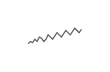
\begin{tikzpicture}[x=0.08em, y=0.08em, line width=0.4pt]
                \draw[FooterGray] (0,3) -- (1,4) -- (2,3.5) -- (3,5) -- (4,4) -- (5,6) -- (6,5.5) -- (7,4) -- (8,5) -- (9,7) -- (10,6) -- (11,5) -- (12,6.5) -- (13,8) -- (14,7) -- (15,6) -- (16,7.5) -- (17,9) -- (18,8) -- (19,7) -- (20,8.5) -- (21,10) -- (22,9) -- (23,8) -- (24,9.5);
            \end{tikzpicture}%
        }%
        \hskip0.5cm%
    }%
    \vskip6pt%
}

%=============================================================================
% PACKAGES
%=============================================================================
\usepackage[utf8]{inputenc}
\DeclareUnicodeCharacter{03B1}{\ensuremath{\alpha}}
\usepackage[T1]{fontenc}
\usepackage{amsmath, amssymb, amsthm}
\usepackage{mathtools}
\usepackage{bm}
\usepackage{tikz}
\usetikzlibrary{arrows.meta, positioning, shapes, calc, decorations.pathreplacing, shadings}
\usepackage{booktabs}
\usepackage{multirow}
\usepackage{array}
\usepackage{graphicx}
\usepackage{animate}
\usepackage{hyperref}
\usepackage{colortbl}
\usepackage{listings}
\lstset{language=Python, basicstyle=\ttfamily\scriptsize, keywordstyle=\color{MainBlue}\bfseries,
  commentstyle=\color{Forest}, stringstyle=\color{Crimson}, breaklines=true,
  frame=none, backgroundcolor=\color{VeryLightGray}, xleftmargin=2mm}
\hypersetup{colorlinks=true, linkcolor=MainBlue, urlcolor=MainBlue}
\graphicspath{{../../logos/}{../../charts/}{../../photos/}}
\usepackage{xcolor}
\hfuzz=2pt  % Suppress tiny overfull warnings (<2pt)
\vfuzz=2pt  % Suppress tiny vertical overfull warnings (<2pt)
% \mathrm in the sans-serif family of the slides (beamer resets \mathrm to the serif family at \begin{document};
% this hook runs after beamer's, so WN, Var, RMSE, ... in formulas match the surrounding text)
% Bold vectors and matrices in the same sans-serif family: \mathbf{A} in sans bold (beamer's own \mathbf came out in
% medium weight), and the bold upright Greek capitals of \boldsymbol / \bm (\bSigma, \bPhi, \boldsymbol{\Theta}) in
% cmss bold: bm.sty fixes its "boldoperators" font when it is loaded (serif cmbx), before beamer switches the
% operators to cmss, so it is reset here.
\AtBeginDocument{%
  \SetMathAlphabet{\mathrm}{normal}{\encodingdefault}{\sfdefault}{\mddefault}{n}%
  \SetMathAlphabet{\mathrm}{bold}{\encodingdefault}{\sfdefault}{bx}{n}%
  \SetMathAlphabet{\mathbf}{normal}{\encodingdefault}{\sfdefault}{bx}{n}%
  \SetMathAlphabet{\mathbf}{bold}{\encodingdefault}{\sfdefault}{bx}{n}%
  \SetSymbolFont{boldoperators}{normal}{OT1}{cmss}{bx}{n}%
  \SetSymbolFont{boldoperators}{bold}{OT1}{cmss}{bx}{n}}

%=============================================================================
% QUANTLET COMMANDS
%   \quantlet{<displayed name>}{<url>}       (generic, compatible with the older TSA decks)
%   \tsaquantlet{Ch_05}{TSA_ch5_garch}       -> https://github.com/danpele/Time-Series-Analysis/tree/main/Quantlets/Ch_05/TSA_ch5_garch
%   \qlurl{<folder>} is defined per chapter by the generator (Quantlets/Ch_NN/<folder>)
%=============================================================================
\newcommand{\tsarepo}{https://github.com/danpele/Time-Series-Analysis}
\newcommand{\tsaqlbase}{https://github.com/danpele/Time-Series-Analysis/tree/main/Quantlets}
\newcommand{\quantlet}[2]{%
    \hfill\href{#2}{%
        \raisebox{-0.15em}{
\includegraphics[height=0.7em]{ql_logo.png}}%
        \textcolor{MainBlue}{\tiny\ #1}%
    }%
}
\newcommand{\tsaquantlet}[2]{\quantlet{\detokenize{#2}}{\tsaqlbase/#1/#2}}

%=============================================================================
% NOTEBOOKS (Google Colab)
%   \colaburl{notebooks/EN/chapter5_seminar_notebook.ipynb} -> the Colab link of a file in the TSA repo
%   \nb: the chapter notebook (each seminar deck redefines it with \renewcommand)
%=============================================================================
\newcommand{\colaburl}[1]{https://colab.research.google.com/github/danpele/Time-Series-Analysis/blob/main/#1}
\newcommand{\nb}{https://colab.research.google.com/github/danpele/Time-Series-Analysis/tree/main/notebooks/EN}
\newcommand{\nbname}{notebooks/EN}

%=============================================================================
% SLIDE HELPERS (used by the generators; the same as in MFM)
%=============================================================================
% local font size for list bodies (the preamble forces \normalsize)
\newcommand{\itemsize}[1]{\setbeamertemplate{itemize/enumerate body begin}{#1}\setbeamertemplate{itemize/enumerate subbody begin}{#1}}
\newcommand{\intitle}[1]{{\hypersetup{urlcolor=white}#1}}   % white links inside coloured title bars
\newcommand{\imgcap}[1]{{\scriptsize #1}\\[0.5mm]}          % caption under a photo
\newcommand{\imgcredit}[2]{{\tiny\color{FooterGray}\href{#1}{#2}}}   % image credit: source URL, author/licence
\newcommand{\aiprompt}[1]{{\ttfamily\color{MainBlue}#1}}     % a prompt to an AI assistant

%=============================================================================
% SEMINARS: student version by default; the instructor wrapper *_solutions.tex sets \solutionstrue
%=============================================================================
\makeatletter\@ifundefined{ifsolutions}{\expandafter\newif\csname ifsolutions\endcsname}{}\makeatother
\newcommand{\solonly}[1]{\ifsolutions #1\fi}
\newcommand{\propsub}{\ifsolutions\else\framesubtitle{\ifdefined\tsalang Rezolvarea se discută la seminar\else Solution discussed in class\fi}\fi}

%=============================================================================
% APPENDIX AND CHAPTER LINKS (latex/appendix_links.py writes the calls; it also re-declares these
% macros before \begin{document}, so the decks compile with or without this preamble block)
%=============================================================================
\providecommand{\tsaapplink}[3]{\hypertarget{#2}{}\hyperlink{#1}{\beamergotobutton{#3}}}
\providecommand{\tsaappback}[2]{\begin{tikzpicture}[remember picture,overlay]\node[anchor=south east] at ([xshift=-3mm,yshift=7mm]current page.south east){\hyperlink{#1}{\beamerreturnbutton{#2}}};\end{tikzpicture}}
\providecommand{\tsachlink}[2]{\href{#1}{#2}}
\providecommand{\tsachlinkt}[2]{\href{#1}{\usebeamercolor[fg]{frametitle}#2}}

%=============================================================================
% QUANTINAR COMMAND: link către un curs Quantinar (subiecte avansate)
%=============================================================================
\newcommand{\quantinar}[2]{%
    \href{#2}{%
        \raisebox{-0.15em}{
\includegraphics[height=0.8em]{qr_logo.png}}%
        \textcolor{MainBlue}{\scriptsize\ #1}%
    }%
}

%=============================================================================
% CUSTOM TITLE PAGE
%=============================================================================
\defbeamertemplate*{title page}{hybrid}[1][]
{
    \vspace{0.2cm}
    % Logos row - top header (with clickable links)
    \begin{center}
        \href{https://www.ase.ro}{
\includegraphics[height=1.0cm]{ase_logo.png}}\hspace{0.3cm}%
        \href{https://theida.net}{
\includegraphics[height=1.0cm]{ida_logo.png}}\hspace{0.3cm}%
        \href{https://blockchain-research-center.com}{
\includegraphics[height=1.0cm]{brc_logo.png}}\hspace{0.3cm}%
        \href{https://www.ai4efin.ase.ro}{
\includegraphics[height=1.0cm]{ai4efin_logo.png}}\hspace{0.3cm}%
        \href{https://ipe.ro/new}{
\includegraphics[height=1.0cm]{acad_logo.png}}\hspace{0.3cm}%
        \href{https://www.digital-finance-msca.com}{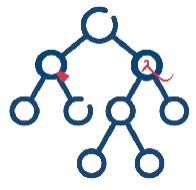
\includegraphics[height=1.0cm]{msca_logo.png}}%
    \end{center}

    \vspace{0.6cm}

    % Main title with Q logos on sides (with clickable links)
    \begin{center}
        \begin{minipage}{0.1\textwidth}
            \centering
            \href{https://quantlet.com}{
\includegraphics[height=1.1cm]{ql_logo.png}}
        \end{minipage}%
        \begin{minipage}{0.78\textwidth}
            \centering
            {\LARGE\bfseries\usebeamercolor[fg]{title}\inserttitle}

            \vspace{0.3cm}

            {\usebeamerfont{subtitle}\usebeamercolor[fg]{title}\insertsubtitle}
        \end{minipage}%
        \begin{minipage}{0.1\textwidth}
            \centering
            \href{https://quantinar.com}{
\includegraphics[height=1.1cm]{qr_logo.png}}
        \end{minipage}
    \end{center}

    \vspace{0.6cm}

    % Authors (left aligned)
    \hspace{0.5cm}{\usebeamerfont{author}\insertauthor}

    \vspace{0.3cm}

    % Institute/Affiliations (left aligned)
    \hspace{0.5cm}\begin{minipage}[t]{0.9\textwidth}
        \raggedright\small\insertinstitute
    \end{minipage}
}

%=============================================================================
% THEOREM ENVIRONMENTS
%=============================================================================
\theoremstyle{definition}
\setbeamertemplate{theorems}[numbered]
\ifdefined\tsalang
\newtheorem{defn}{Definiție}
\newtheorem{thm}{Teoremă}
\newtheorem{prop}{Propoziție}
\newtheorem{rmk}{Observație}
\else
\newtheorem{defn}{Definition}
\newtheorem{thm}{Theorem}
\newtheorem{prop}{Proposition}
\newtheorem{rmk}{Remark}
\fi

%=============================================================================
% CENTRED MINIPAGE (no extra vertical space)
%=============================================================================
\newenvironment{cminipage}[1]{%
    \par\noindent\hfill\begin{minipage}{#1}\ignorespaces
}{%
    \end{minipage}\hfill\null\par
}

%=============================================================================
% CUSTOM COMMANDS
%=============================================================================
\newcommand{\E}{\mathbb{E}}
\newcommand{\Var}{\text{Var}}
\newcommand{\Cov}{\text{Cov}}
\newcommand{\Corr}{\text{Corr}}
\newcommand{\R}{\mathbb{R}}
\newcommand{\N}{\mathbb{N}}
\newcommand{\Z}{\mathbb{Z}}
\newcommand{\B}{\mathbf{B}}
\newcommand{\imark}{\textcolor{MainBlue}{\textbullet}}
\newcommand{\RMSE}{\text{RMSE}}
\newcommand{\MAE}{\text{MAE}}
\newcommand{\MAPE}{\text{MAPE}}

% Boldface vector/matrix commands (VAR, VECM, state space; also used by the older TSA decks)
\newcommand{\bY}{\mathbf{Y}}
\newcommand{\bX}{\mathbf{X}}
\newcommand{\bA}{\mathbf{A}}
\newcommand{\bB}{\mathbf{B}}
\newcommand{\bepsilon}{\boldsymbol{\varepsilon}}
\newcommand{\bSigma}{\boldsymbol{\Sigma}}
\newcommand{\bPhi}{\boldsymbol{\Phi}}
\newcommand{\bGamma}{\boldsymbol{\Gamma}}
\newcommand{\bPi}{\boldsymbol{\Pi}}
\newcommand{\bc}{\mathbf{c}}
\newcommand{\balpha}{\boldsymbol{\alpha}}
\newcommand{\bbeta}{\boldsymbol{\beta}}
\newcommand{\bvarepsilon}{\boldsymbol{\varepsilon}}

% Legacy seminar marks (older TSA seminar decks)
\newcommand{\correct}{\textcolor{Forest}{\checkmark}}
\newcommand{\incorrect}{\textcolor{Crimson}{\texttimes}}


\newcommand{\qlurl}[1]{https://github.com/danpele/Time-Series-Analysis/tree/main/Quantlets/Ch_05/#1}

% Clickable citations (DOIs verified via Crossref)
\newcommand{\refHP}{\href{https://doi.org/10.1007/978-3-031-13584-2}{Huang and Petukhina (2022)}}
\newcommand{\refFPP}{\href{https://otexts.com/fpp3/}{Hyndman and Athanasopoulos (2021)}}
\newcommand{\refTsay}{\href{https://doi.org/10.1002/9780470644560}{Tsay (2010)}}
\newcommand{\refFHH}{\href{https://doi.org/10.1007/978-3-030-13751-9}{Franke, Härdle and Hafner (2019)}}
\newcommand{\refHamilton}{\href{https://doi.org/10.2307/j.ctv14jx6sm}{Hamilton (1994)}}
\newcommand{\refEngle}{\href{https://doi.org/10.2307/1912773}{Engle (1982)}}
\newcommand{\refEngleN}{\href{https://doi.org/10.1257/0002828041464597}{Engle (2004)}}
\newcommand{\refBoll}{\href{https://doi.org/10.1016/0304-4076(86)90063-1}{Bollerslev (1986)}}
\newcommand{\refBollT}{\href{https://doi.org/10.2307/1925546}{Bollerslev (1987)}}
\newcommand{\refEB}{\href{https://doi.org/10.1080/07474938608800095}{Engle and Bollerslev (1986)}}
\newcommand{\refNelson}{\href{https://doi.org/10.2307/2938260}{Nelson (1991)}}
\newcommand{\refGJR}{\href{https://doi.org/10.1111/j.1540-6261.1993.tb05128.x}{Glosten, Jagannathan and Runkle (1993)}}
\newcommand{\refEN}{\href{https://doi.org/10.1111/j.1540-6261.1993.tb05127.x}{Engle and Ng (1993)}}
\newcommand{\refBW}{\href{https://doi.org/10.1080/07474939208800229}{Bollerslev and Wooldridge (1992)}}
\newcommand{\refHansen}{\href{https://doi.org/10.2307/2527081}{Hansen (1994)}}
\newcommand{\refPatton}{\href{https://doi.org/10.1016/j.jeconom.2010.03.034}{Patton (2011)}}
\newcommand{\refHL}{\href{https://doi.org/10.1002/jae.800}{Hansen and Lunde (2005)}}
\newcommand{\refAB}{\href{https://doi.org/10.2307/2527343}{Andersen and Bollerslev (1998)}}
\newcommand{\refChristie}{\href{https://doi.org/10.1016/0304-405X(82)90018-6}{Christie (1982)}}
\newcommand{\refDM}{\href{https://doi.org/10.1080/07350015.1995.10524599}{Diebold and Mariano (1995)}}
\newcommand{\refLB}{\href{https://doi.org/10.1093/biomet/65.2.297}{Ljung and Box (1978)}}
\newcommand{\refML}{\href{https://doi.org/10.1111/j.1467-9892.1983.tb00373.x}{McLeod and Li (1983)}}
\newcommand{\refMandelbrot}{\href{https://doi.org/10.1086/294632}{Mandelbrot (1963)}}
\newcommand{\refRM}{\href{https://www.msci.com/documents/10199/5915b101-4206-4ba0-aee2-3449d5c7e95a}{J.P. Morgan/Reuters (1996)}}
\newcommand{\refAkaike}{\href{https://doi.org/10.1109/TAC.1974.1100705}{Akaike (1974)}}
\newcommand{\refSchwarz}{\href{https://doi.org/10.1214/aos/1176344136}{Schwarz (1978)}}
\newcommand{\refKupiec}{\href{https://doi.org/10.3905/jod.1995.407942}{Kupiec (1995)}}

\title[Time Series Analysis]{Time Series Analysis}
\subtitle{Chapter 5: Conditional volatility: ARCH and GARCH}
\author[D.T. Pele]{Daniel Traian PELE}
\institute{Bucharest University of Economic Studies\\
IDA Institute Digital Assets\\
Blockchain Research Center\\
AI4EFin Artificial Intelligence for Energy Finance\\
Romanian Academy, Institute for Economic Forecasting\\
MSCA Digital Finance}
\date{}

%=============================================================================
\providecommand{\tsaapplink}[3]{\hypertarget{#2}{}\hyperlink{#1}{\beamergotobutton{#3}}}  % APPLINKS-MACROS
\providecommand{\tsaappback}[2]{\begin{tikzpicture}[remember picture,overlay]\node[anchor=south east] at ([xshift=-3mm,yshift=7mm]current page.south east){\hyperlink{#1}{\beamerreturnbutton{#2}}};\end{tikzpicture}}  % APPLINKS-MACROS
\providecommand{\tsachlink}[2]{\href{#1}{#2}}  % APPLINKS-MACROS
\providecommand{\tsachlinkt}[2]{\href{#1}{\usebeamercolor[fg]{frametitle}#2}}  % APPLINKS-MACROS
\begin{document}
%=============================================================================

{
\setbeamertemplate{headline}{}
\setbeamertemplate{footline}{}
\begin{frame}[noframenumbering]
    \titlepage
\end{frame}
}
% BEGIN-ACRONYMS (generat de latex/acronyms.py; nu editati manual)
\begin{frame}{Acronyms used in this material (1/2)}
\setbeamertemplate{itemize/enumerate body begin}{\tiny}
\begin{columns}[T]
\begin{column}{0.49\textwidth}
\begin{itemize}\setlength{\itemsep}{0pt}
    \item \textbf{ACF}: Autocorrelation Function
    \item \textbf{AI}: Artificial Intelligence
    \item \textbf{AIC}: Akaike Information Criterion
    \item \textbf{AR}: AutoRegressive (model); in event studies: Abnormal Return
    \item \textbf{AR-GARCH}: AR model for the mean with GARCH errors
    \item \textbf{ARCH}: AutoRegressive Conditional Heteroskedasticity
    \item \textbf{ARCH-LM}: ARCH Lagrange Multiplier (test)
    \item \textbf{ARMA}: AutoRegressive Moving Average (model)
    \item \textbf{ARMA-GARCH}: ARMA model for the mean with GARCH errors
    \item \textbf{BET}: Bucharest Exchange Trading (index)
    \item \textbf{BIC}: Bayesian Information Criterion
    \item \textbf{BNR}: Banca Națională a României (the National Bank of Romania)
    \item \textbf{BVB}: Bursa de Valori București (the Bucharest Stock Exchange)
\end{itemize}
\end{column}
\begin{column}{0.49\textwidth}
\begin{itemize}\setlength{\itemsep}{0pt}
    \item \textbf{COVID-19}: COronaVIrus Disease 2019
    \item \textbf{DM}: Diebold–Mariano (test)
    \item \textbf{EGARCH}: Exponential GARCH
    \item \textbf{EWMA}: Exponentially Weighted Moving Average
    \item \textbf{GARCH}: Generalised AutoRegressive Conditional Heteroskedasticity
    \item \textbf{GARCH-N}: GARCH with Normal innovations
    \item \textbf{GJR}: Glosten–Jagannathan–Runkle (GARCH model)
    \item \textbf{GJR-GARCH}: Glosten–Jagannathan–Runkle GARCH
    \item \textbf{HAC}: Heteroskedasticity and Autocorrelation Consistent (standard errors)
    \item \textbf{IGARCH}: Integrated GARCH
    \item \textbf{LM}: Lagrange Multiplier
    \item \textbf{LR}: Likelihood Ratio (test)
    \item \textbf{MA}: Moving Average
\end{itemize}
\end{column}
\end{columns}
\end{frame}
\begin{frame}{Acronyms used in this material (2/2)}
\setbeamertemplate{itemize/enumerate body begin}{\tiny}
\begin{columns}[T]
\begin{column}{0.49\textwidth}
\begin{itemize}\setlength{\itemsep}{0pt}
    \item \textbf{MLE}: Maximum Likelihood Estimation
    \item \textbf{NIC}: News Impact Curve
    \item \textbf{OLS}: Ordinary Least Squares
    \item \textbf{PACF}: Partial AutoCorrelation Function
    \item \textbf{QLIKE}: Quasi-LIKElihood (loss function)
    \item \textbf{QMLE}: Quasi-Maximum Likelihood Estimation
    \item \textbf{QQ}: Quantile–Quantile (plot)
    \item \textbf{SE}: Standard Error
    \item \textbf{US}: United States
    \item \textbf{VAR}: Vector AutoRegression
\end{itemize}
\end{column}
\begin{column}{0.49\textwidth}
\end{column}
\end{columns}
\end{frame}
% END-ACRONYMS

\begin{frame}{Today's question and route}
\itemsize{\small}
\begin{itemize}
    \item \textbf{Question}: if tomorrow's return cannot be predicted, can tomorrow's \textbf{risk} be predicted?
    \begin{itemize}
        \item \tsachlink{https://danpele.github.io/Time-Series-Analysis/EN/Courses/chapter1_stochastic_processes_stationarity.pdf}{Chapters 1}--\tsachlink{https://danpele.github.io/Time-Series-Analysis/EN/Courses/chapter3_unit_roots_arima_models.pdf}{3} modelled the conditional \textbf{mean} of a series; this chapter models its conditional \textbf{variance}
    \end{itemize}
    \item \textbf{Route} of the chapter
    \begin{itemize}
        \item stylised facts of returns; the ACF of squared returns and the ARCH-LM test
        \item conditional mean and conditional variance; ARCH($q$) and GARCH(1,1); persistence, IGARCH and EWMA
        \item estimation by maximum likelihood with the \texttt{arch} package; Student-t innovations; ARMA-GARCH models
        \item asymmetry (GJR, EGARCH), diagnostics, variance forecasts and their evaluation, VaR 1\%
    \end{itemize}
    \item Data: S\&P 500, BET, EUR/RON (BNR reference rate) and Bitcoin, daily; Seminar 5 comes before this lecture
\end{itemize}
\end{frame}

\begin{frame}{Learning outcomes}
\itemsize{\small}
\begin{itemize}
    \item List the stylised facts of financial returns and test for ARCH effects with the ACF of squared returns and the ARCH-LM test
    \item Distinguish the conditional from the unconditional variance, and explain why returns can be uncorrelated yet dependent
    \item Write ARCH($q$), GARCH(1,1) and ARMA-GARCH models; compute the persistence, the long-run variance and the half-life
    \item Estimate GARCH models by maximum likelihood in Python, choose the innovation distribution and check the standardised residuals
    \item Measure asymmetry with GJR-GARCH, EGARCH and the news impact curve
    \item Forecast the variance over several horizons, evaluate the forecasts with QLIKE and compute a one-day VaR 1\%
\end{itemize}
\end{frame}

\begin{frame}{Reading and tools}
\itemsize{\small}
\begin{itemize}
    \item Textbook: \refHP, Ch.~6 (financial time series: ARCH and GARCH models)
    \begin{itemize}
        \item further reading: \refTsay, Ch.~3; \refFHH, Ch.~13
    \end{itemize}
    \item Theory: \refHamilton, Ch.~21 (time series models of heteroskedasticity)
    \item Python Quantlets of this chapter: \href{https://github.com/danpele/Time-Series-Analysis/tree/main/Quantlets/Ch_05}{Quantlets/Ch\_05}
    \begin{itemize}
        \item estimation with the package \texttt{arch} (install it in Colab with \texttt{pip install arch}); tests with \texttt{statsmodels}
    \end{itemize}
    \item Lecture notebook: \href{\colaburl{notebooks/EN/chapter5_lecture_notebook.ipynb}}{open in Google Colab}
    \item Video course: \quantinar{Applied Time Series Analysis with Python}{https://quantinar.com/course/137/applied-time-series-analysis-with-python}
\end{itemize}
\end{frame}


%=============================================================================
\section{Stylised facts of financial returns}
%=============================================================================

\begin{frame}{Four markets, one pattern}
\itemsize{\footnotesize}
\begin{center}
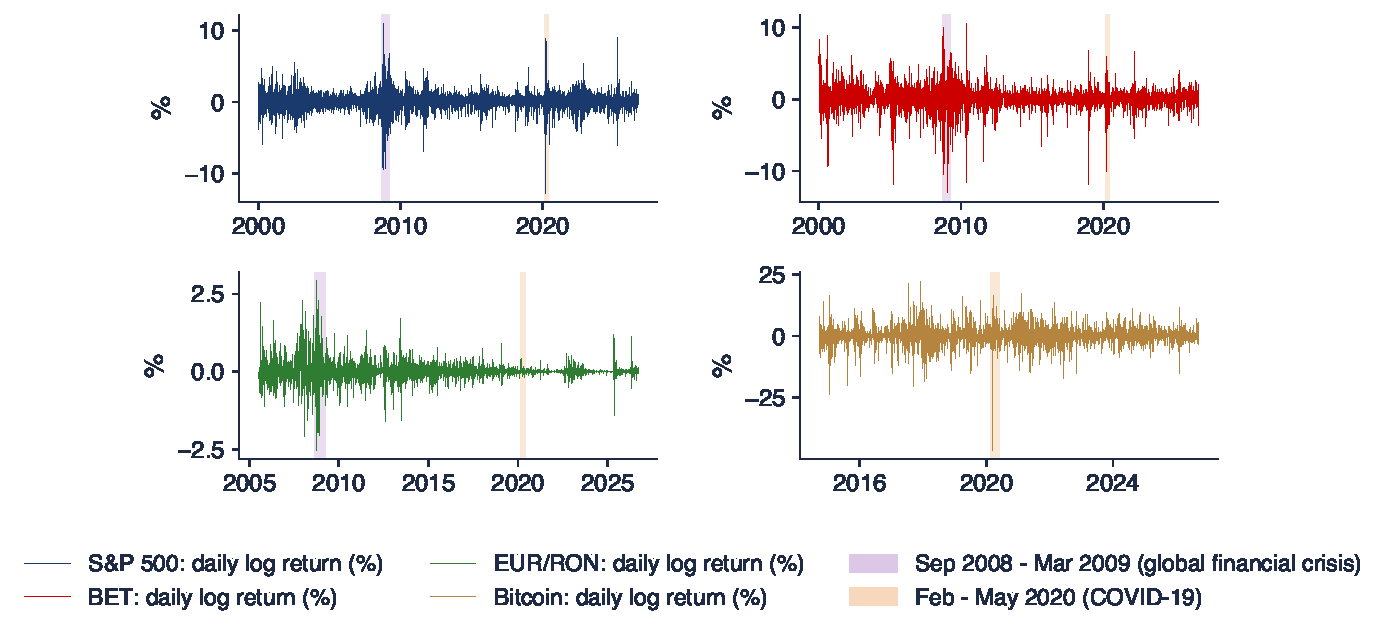
\includegraphics[width=0.97\textwidth,height=0.64\textheight,keepaspectratio]{tsa_ch5_returns.pdf}
\end{center}
\vspace{-0.25cm}
\begin{itemize}
    \item Daily log returns $r_t = 100(\ln P_t - \ln P_{t-1})$, in \%, to 18 September 2026: S\&P 500 and BET since 2000, EUR/RON (BNR reference rate) since July 2005, Bitcoin since September 2014
    \item Shaded: the global financial crisis (September 2008 -- March 2009) and the COVID-19 crash (February -- May 2020)
\end{itemize}
\quantlet{TSA\_ch5\_stylised\_facts}{\qlurl{TSA_ch5_stylised_facts}}
\end{frame}

\begin{frame}{Interpreting the four series}
\itemsize{\small}
\begin{itemize}
    \item Calm years alternate with storms: large changes follow large changes, of either sign
    \begin{itemize}
        \item this is \textbf{volatility clustering}, first described by \refMandelbrot
    \end{itemize}
    \item S\&P 500: daily standard deviation 0.42\% in 2017, 3.52\% from September 2008 to March 2009 ($\times$8.3) and 3.70\% in February--May 2020 ($\times$8.8)
    \item EUR/RON: 0.78\% in the 2008 crisis, only 0.10\% in 2020: the BNR kept the leu almost fixed
    \item A model with a constant variance (white noise, \tsachlink{https://danpele.github.io/Time-Series-Analysis/EN/Courses/chapter1_stochastic_processes_stationarity.pdf}{Chapter 1}) describes none of these series
\end{itemize}
\end{frame}

\begin{frame}{Two storms: 2008 and 2020}
\itemsize{\footnotesize}
\begin{columns}[T]
\begin{column}{0.48\textwidth}
\centering
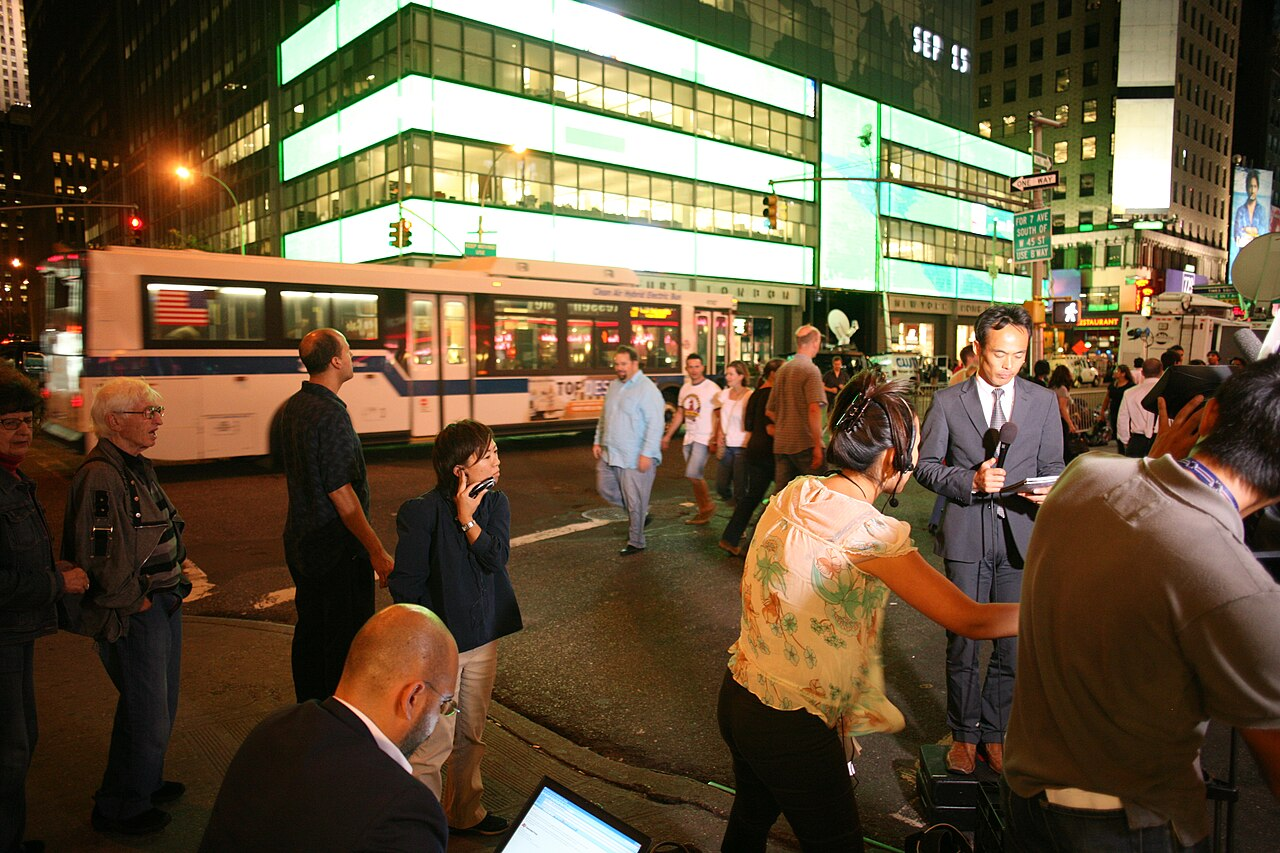
\includegraphics[height=0.42\textheight]{ch5_lehman_2008.jpg}\\[1mm]
\imgcap{Lehman Brothers headquarters, New York, 15 September 2008}
\imgcredit{https://commons.wikimedia.org/wiki/File:Lehman_Brothers-NYC-20080915.jpg}{Photo: Robert Scoble (2008); CC BY 2.0; Wikimedia Commons}
\end{column}
\begin{column}{0.48\textwidth}
\centering
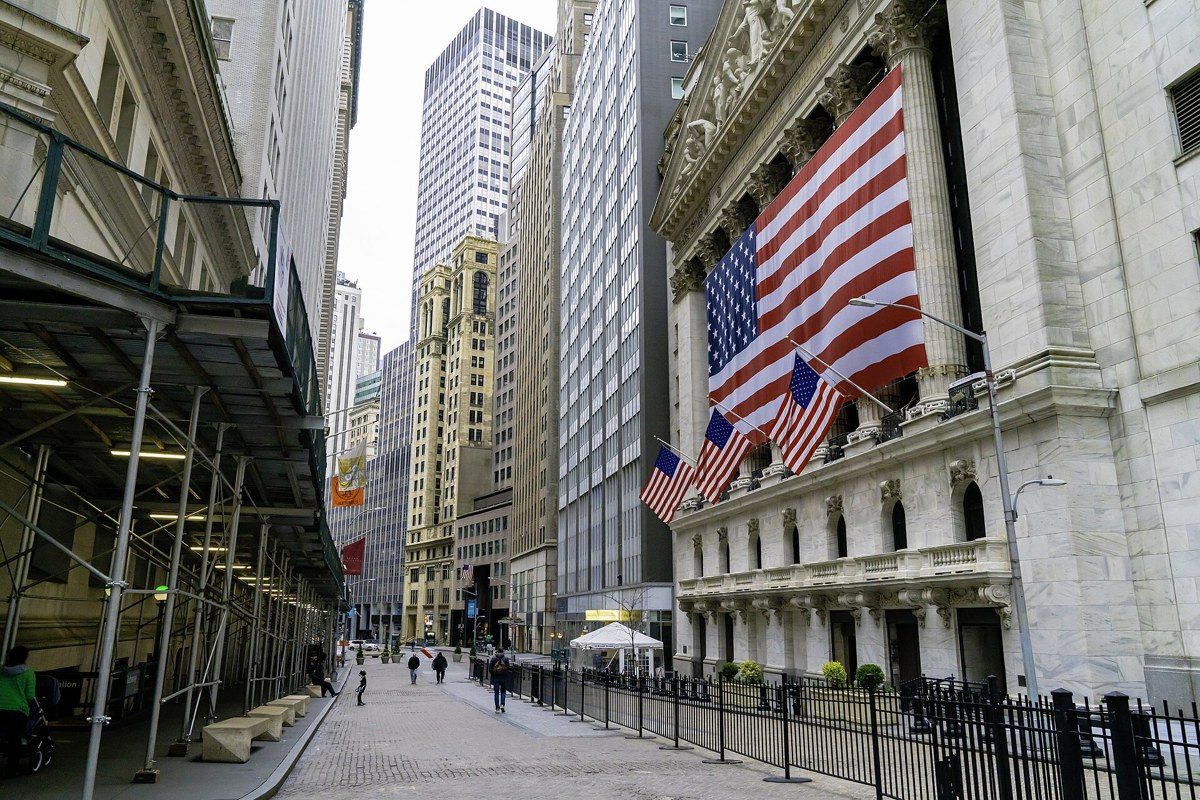
\includegraphics[height=0.42\textheight]{ch5_fidi_2020.jpg}\\[1mm]
\imgcap{The Financial District of New York, 25 March 2020}
\imgcredit{https://commons.wikimedia.org/wiki/File:Subdued_FiDi_(50063555551).jpg}{Photo: Billie Grace Ward (2020); CC BY 2.0; Wikimedia Commons}
\end{column}
\end{columns}\begin{itemize}
    \item 15 September 2008: Lehman Brothers files for bankruptcy; March 2020: the COVID-19 pandemic closes economies
    \item In both episodes calm returned only after months: a shock to volatility is persistent
\end{itemize}
\end{frame}

\begin{frame}{Stylised facts in numbers}
\itemsize{\footnotesize}
\begin{center}
\scriptsize
\begin{tabular}{lrrrrrrrrr}
\toprule
& $T$ & s.d. & skew. & kurt. & $\hat\rho_1(r)$ & $\hat\rho_1(r^2)$ & $Q(10)$, $r$ & $Q(10)$, $r^2$ & LM(5) \\
\midrule
S\&P 500 & 6\,714 & $1.21$ & $-0.35$ & $13.7$ & $-0.10$ & $0.31$ & 96 & 6133 & 1684 \\
BET & 6\,670 & $1.40$ & $-0.65$ & $14.1$ & $0.11$ & $0.33$ & 108 & 2440 & 982 \\
EUR/RON & 5\,352 & $0.28$ & $0.73$ & $18.1$ & $0.17$ & $0.34$ & 222 & 2420 & 871 \\
Bitcoin & 4\,384 & $3.49$ & $-0.70$ & $15.0$ & $-0.02$ & $0.14$ & 20 & 213 & 115 \\
\bottomrule
\end{tabular}
\end{center}
\begin{itemize}
    \item \textbf{Heavy tails}: kurtosis between 13.7 and 18.1, far above 3, the value of the Normal distribution
    \begin{itemize}
        \item kurtosis $K = E[(r - \mu)^4]/\sigma^4$; skewness $E[(r - \mu)^3]/\sigma^3$ (\tsachlink{https://danpele.github.io/Time-Series-Analysis/EN/Courses/chapter1_stochastic_processes_stationarity.pdf}{Chapter 1})
    \end{itemize}
    \item \textbf{Little autocorrelation in $r_t$}, strong autocorrelation in $r_t^2$: $Q(10)$ of the squares is 11--64 times larger
    \item $Q(10)$: the Ljung--Box statistic \refLB\ (\tsachlink{https://danpele.github.io/Time-Series-Analysis/EN/Courses/chapter1_stochastic_processes_stationarity.pdf}{Chapter 1}), $\chi^2(10)$, 5\% value 18.31; LM(5): the ARCH-LM test (two slides ahead), $\chi^2(5)$, 5\% value 11.07
\end{itemize}\quantlet{TSA\_ch5\_stylised\_facts}{\qlurl{TSA_ch5_stylised_facts}}
\end{frame}

\begin{frame}{The sign is unpredictable, the size is not}
\itemsize{\footnotesize}
\begin{center}
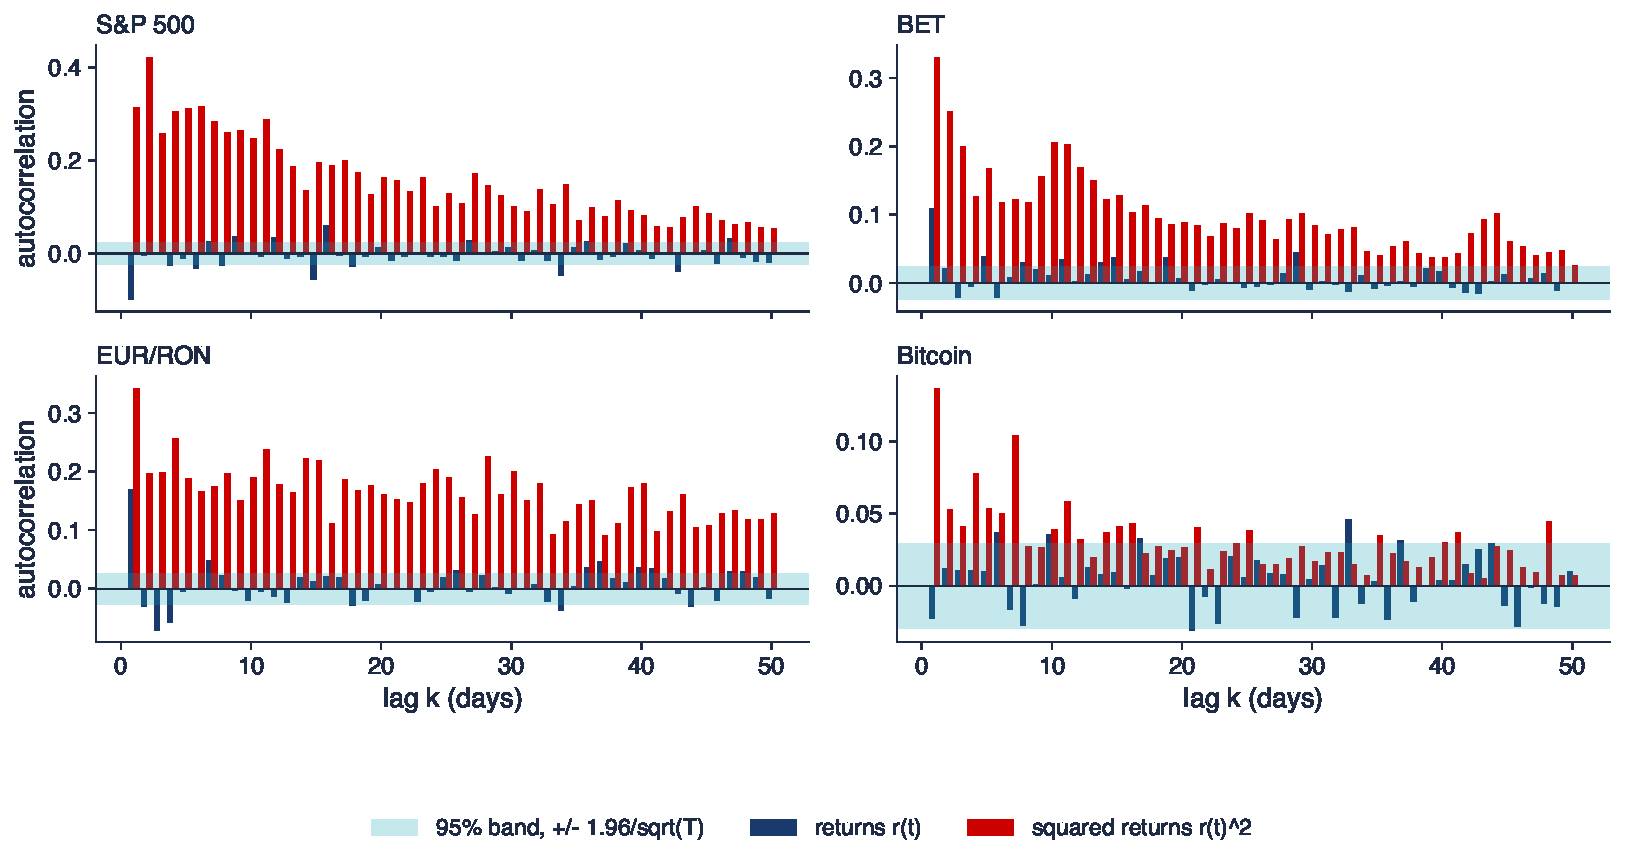
\includegraphics[width=0.97\textwidth,height=0.56\textheight,keepaspectratio]{tsa_ch5_acf_squares.pdf}
\end{center}
\vspace{-0.25cm}
\begin{itemize}
    \item Sample ACF (autocorrelation function, \tsachlink{https://danpele.github.io/Time-Series-Analysis/EN/Courses/chapter1_stochastic_processes_stationarity.pdf}{Chapter 1}) of $r_t$ and of $r_t^2$, lags 1--50, with the band $\pm 1.96/\sqrt{T}$ of an i.i.d.\ (independent and identically distributed) series
\end{itemize}
\quantlet{TSA\_ch5\_stylised\_facts}{\qlurl{TSA_ch5_stylised_facts}}
\end{frame}

\begin{frame}{Interpreting the two ACFs}
\itemsize{\small}
\begin{itemize}
    \item Returns: almost all autocorrelations inside the band (BET: $\hat\rho_1 = 0.11$, a thin market; \tsachlink{https://danpele.github.io/Time-Series-Analysis/EN/Courses/chapter2_arma_models.pdf}{Chapter 2})
    \begin{itemize}
        \item the direction of tomorrow's move is almost unpredictable
    \end{itemize}
    \item Squared returns: S\&P 500 0.31 at lag 1 and still 0.05 at lag 50; 50 of 50 lags outside the band
    \begin{itemize}
        \item the size of tomorrow's move is predictable: a large move today makes a large move tomorrow more likely
    \end{itemize}
    \item Uncorrelated is not the same as independent: $r_t$ is close to white noise but not i.i.d. (\tsachlink{https://danpele.github.io/Time-Series-Analysis/EN/Courses/chapter1_stochastic_processes_stationarity.pdf}{Chapter 1})
    \item Bitcoin: weaker but significant ($\hat\rho_1(r_t^2) = 0.14$): a few huge days dominate the squares
\end{itemize}
\end{frame}

\begin{frame}{Testing for ARCH effects}
\itemsize{\small}
\begin{itemize}
    \item \textbf{ARCH effects}: the conditional variance depends on the past (the name comes from the ARCH model, Section 3)
    \item \textbf{Ljung--Box on squares} (the McLeod--Li test \refML): $Q(m) = T(T+2)\sum_{k=1}^{m}\hat\rho_k^2(\hat\varepsilon^2)/(T-k)$
    \begin{itemize}
        \item $\hat\varepsilon_t$: residuals of the mean model (for returns, $r_t - \bar r$); under $H_0$ (no ARCH effects), $Q(m) \sim \chi^2(m)$
    \end{itemize}
    \item \textbf{ARCH-LM test} \refEngle: LM (Lagrange multiplier) test from the auxiliary regression
    \begin{itemize}
        \item $\hat\varepsilon_t^2 = b_0 + b_1\hat\varepsilon_{t-1}^2 + \dots + b_q\hat\varepsilon_{t-q}^2 + u_t$, estimated by OLS (ordinary least squares)
        \item $H_0$: $b_1 = \dots = b_q = 0$; $\mathrm{LM} = n R^2 \sim \chi^2(q)$, $n$ = number of observations in the regression
    \end{itemize}
    \item Both tests are run on the residuals of the mean model, before and after fitting a volatility model
\end{itemize}
\end{frame}

\begin{frame}{Worked example: ARCH-LM on the BET}
\itemsize{\footnotesize}
\begin{itemize}
    \item Mean model: AR(1) for the BET returns (\tsachlink{https://danpele.github.io/Time-Series-Analysis/EN/Courses/chapter2_arma_models.pdf}{Chapter 2}), $\hat\phi = 0.109$; residuals $\hat\varepsilon_t$; $q = 5$
    \item Auxiliary regression (OLS)
    \begin{itemize}
        \item $\hat\varepsilon_t^2 = 0.862 + 0.276\,\hat\varepsilon_{t-1}^2 + 0.099\,\hat\varepsilon_{t-2}^2 + 0.088\,\hat\varepsilon_{t-3}^2 + (-0.015)\,\hat\varepsilon_{t-4}^2 + 0.102\,\hat\varepsilon_{t-5}^2$
        \item $R^2 = 0.153$, $n = 6\,664$
    \end{itemize}
    \item Step by step: $\mathrm{LM} = n R^2 = 6\,664 \times 0.153 = 1017$; 5\% critical value $\chi^2_{0.95}(5) = 11.07$
    \begin{itemize}
        \item $1017 \gg 11.07$: reject $H_0$; the variance of the BET depends on the last five squared shocks
    \end{itemize}
    \item Interpretation: $R^2 = 0.153$ is small, but for squared returns it is a strong signal; the model of the variance is the next step
\end{itemize}\quantlet{TSA\_ch5\_mean\_model}{\qlurl{TSA_ch5_mean_model}}
\end{frame}

\begin{frame}{Recap: stylised facts}
\itemsize{\small}
\begin{itemize}
    \item Heavy tails, volatility clustering, little autocorrelation in $r_t$, strong autocorrelation in $r_t^2$
    \item ARCH effects: Ljung--Box on squared residuals, ARCH-LM $= nR^2 \sim \chi^2(q)$
    \item All four series reject $H_0$ by a wide margin
\end{itemize}
\end{frame}


%=============================================================================
\section{Conditional mean and conditional variance}
%=============================================================================

\begin{frame}{Conditioning on the past}
\itemsize{\small}
\begin{itemize}
    \item $\mathcal{F}_{t-1}$: the information available at the end of day $t-1$ (all past values)
    \begin{itemize}
        \item conditional expectation $E[X \mid \mathcal{F}_{t-1}]$: the best forecast of $X$ given the past (\tsachlink{https://danpele.github.io/Time-Series-Analysis/EN/Courses/chapter2_arma_models.pdf}{Chapter 2})
    \end{itemize}
    \item \textbf{Conditional mean}: $\mu_t = E[r_t \mid \mathcal{F}_{t-1}]$
    \begin{itemize}
        \item an ARMA model (\tsachlink{https://danpele.github.io/Time-Series-Analysis/EN/Courses/chapter2_arma_models.pdf}{Chapter 2}) is a model for $\mu_t$; for daily returns $\mu_t$ is small and almost constant
    \end{itemize}
    \item \textbf{Conditional variance}: $\sigma_t^2 = \mathrm{Var}(r_t \mid \mathcal{F}_{t-1}) = E[(r_t - \mu_t)^2 \mid \mathcal{F}_{t-1}]$
    \begin{itemize}
        \item $\sigma_t$ is the \textbf{conditional volatility}: known at $t-1$, it changes from day to day
        \item \textbf{conditional heteroskedasticity}: a conditional variance that is not constant
    \end{itemize}
    \item \textbf{Unconditional variance} $\mathrm{Var}(r_t)$: one number for the whole sample; it can be constant while $\sigma_t^2$ moves
\end{itemize}
\end{frame}

\begin{frame}{The basic decomposition}
\itemsize{\small}
\begin{itemize}
    \item Every model of this chapter: $r_t = \mu_t + \varepsilon_t$, \quad $\varepsilon_t = \sigma_t z_t$
    \begin{itemize}
        \item $z_t$: the \textbf{innovations}, i.i.d.\ with mean 0 and variance 1 (Normal, Student-t, \dots)
        \item $\varepsilon_t$: the \textbf{shock}; $\mu_t$ and $\sigma_t$ depend only on the past
    \end{itemize}
    \item Consequences
    \begin{itemize}
        \item $E[\varepsilon_t \mid \mathcal{F}_{t-1}] = \sigma_t E[z_t] = 0$: the shocks are a \textbf{martingale difference}, hence uncorrelated (white noise)
        \item $\mathrm{Var}(\varepsilon_t \mid \mathcal{F}_{t-1}) = \sigma_t^2$: the variance is predictable
        \item the $\varepsilon_t$ are uncorrelated but not independent: $\varepsilon_t^2$ is correlated with $\varepsilon_{t-1}^2$
    \end{itemize}
    \item Two models, one for each moment: ARMA for $\mu_t$ (\tsachlink{https://danpele.github.io/Time-Series-Analysis/EN/Courses/chapter2_arma_models.pdf}{Chapter 2}), GARCH for $\sigma_t^2$ (this chapter); together: \textbf{ARMA-GARCH}
\end{itemize}
\end{frame}

\begin{frame}{Worked example: conditional and unconditional variance}
\itemsize{\small}
\begin{itemize}
    \item A market has calm days ($\sigma_t^2 = 0.5$) and stormy days ($\sigma_t^2 = 4.5$), each with probability $1/2$; the mean is 0
    \begin{itemize}
        \item law of total variance: $\mathrm{Var}(r_t) = E[\mathrm{Var}(r_t \mid \mathcal{F}_{t-1})] + \mathrm{Var}(E[r_t \mid \mathcal{F}_{t-1}])$
        \item step by step: $0.5 \times 0.5 + 0.5 \times 4.5 + 0 = 2.50$; unconditional standard deviation $1.58\%$
    \end{itemize}
    \item The unconditional variance is an average; the conditional variance tells which day we are in
    \begin{itemize}
        \item a calm day: $\sigma_t = 0.71\%$; a stormy day: $\sigma_t = 2.12\%$; the average $1.58\%$ fits neither
    \end{itemize}
    \item With Normal $z_t$, the mixture has kurtosis $3E[\sigma_t^4]/(E[\sigma_t^2])^2 = 4.92$: a time-varying variance creates heavy tails
\end{itemize}
\end{frame}

\begin{frame}{The mean model leaves ARCH effects}
\itemsize{\footnotesize}
\begin{center}
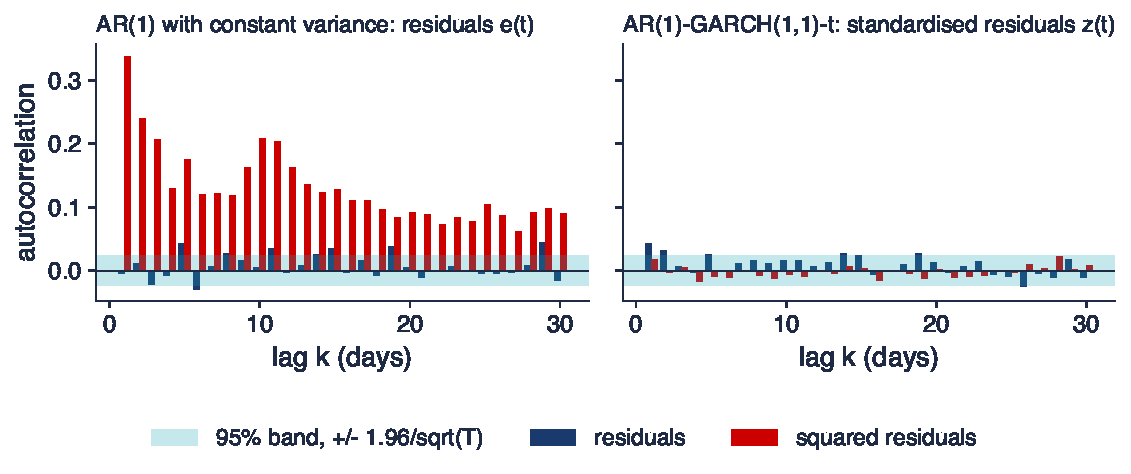
\includegraphics[width=0.97\textwidth,height=0.48\textheight,keepaspectratio]{tsa_ch5_arma_resid.pdf}
\end{center}
\vspace{-0.25cm}
\begin{itemize}
    \item BET: left, an AR(1) for the mean (order chosen by BIC among AR(0)--AR(5): $p = 1$), constant variance; right, the same AR(1) with a GARCH(1,1)-t variance (Section 6)
\end{itemize}
\quantlet{TSA\_ch5\_mean\_model}{\qlurl{TSA_ch5_mean_model}}
\end{frame}

\begin{frame}{Interpreting the residual ACFs}
\itemsize{\small}
\begin{itemize}
    \item Left: the residuals look almost like white noise, the Box--Jenkins check of \tsachlink{https://danpele.github.io/Time-Series-Analysis/EN/Courses/chapter2_arma_models.pdf}{Chapter 2} would be nearly passed
    \begin{itemize}
        \item but their squares: $\hat\rho_1 = 0.34$, $Q(10) = 2496$: strong ARCH effects
    \end{itemize}
    \item Right: after dividing by $\hat\sigma_t$, the squares are clean: $\hat\rho_1 = 0.018$, $Q(10) = 7.2$ (p = 0.705), ARCH-LM 4.8 (p = 0.446)
    \begin{itemize}
        \item some autocorrelation in the level remains ($Q(10) = 28.6$): the BET mean has more structure than an AR(1)
    \end{itemize}
    \item Lesson: check both $\hat\varepsilon_t$ and $\hat\varepsilon_t^2$; a white-noise check on $\hat\varepsilon_t$ alone misses the variance
\end{itemize}
\end{frame}

\begin{frame}{Recap: conditional mean and variance}
\itemsize{\small}
\begin{itemize}
    \item $r_t = \mu_t + \sigma_t z_t$: $\mu_t$ from an ARMA model, $\sigma_t^2$ from a volatility model
    \item Shocks are uncorrelated but dependent through their squares
    \item Unconditional variance = average of the conditional variances; the mixture has heavy tails
\end{itemize}
\end{frame}


%=============================================================================
\section{The ARCH model}
%=============================================================================

\begin{frame}{1982: Robert Engle and ARCH}
\itemsize{\footnotesize}
\begin{columns}[T]
\begin{column}{0.60\textwidth}
\begin{itemize}
    \item \refEngle: \textbf{ARCH} (autoregressive conditional heteroskedasticity): today's variance depends on yesterday's squared shocks
    \begin{itemize}
        \item first application: the variance of inflation in the United Kingdom, not a financial market
    \end{itemize}
    \item \href{https://www.nobelprize.org/prizes/economic-sciences/2003/summary/}{Nobel Prize 2003}: ``for methods of analyzing economic time series with time-varying volatility (ARCH)''
    \begin{itemize}
        \item shared with Clive Granger (\tsachlink{https://danpele.github.io/Time-Series-Analysis/EN/Courses/chapter3_unit_roots_arima_models.pdf}{Chapter 3}: spurious regression; Chapter 7: cointegration); Nobel lecture: \refEngleN
    \end{itemize}
\end{itemize}
\end{column}
\begin{column}{0.36\textwidth}
\centering

\includegraphics[height=0.25\textheight]{ch5_robert_engle_2022.jpg}\\[1mm]
\imgcap{Robert F. Engle (2022)}
\imgcredit{https://commons.wikimedia.org/wiki/File:0603-Kraneshares_KRBN-RobertEngle-JonDemske-16_(cropped).jpg}{Photo: Jon Demske (2022); CC BY-SA 4.0; Wikimedia Commons}\\[1mm]
\centering
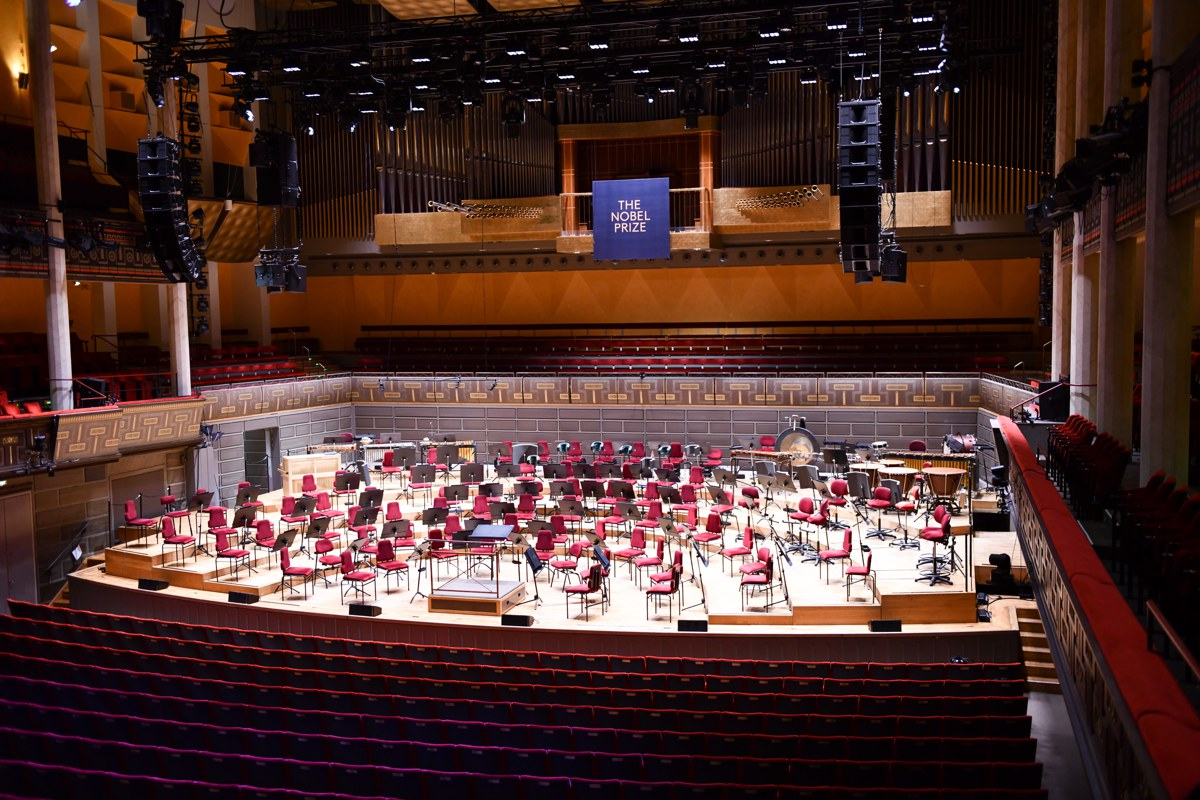
\includegraphics[height=0.16\textheight]{ch5_stockholm_concert_hall.jpg}\\[1mm]
\imgcap{Stockholm Concert Hall, venue of the Nobel Prize ceremony}
\imgcredit{https://commons.wikimedia.org/wiki/File:Konserthuset_Stockholm_(Stockholm_Concert_Hall).jpg}{Photo: Karen Zhou (2025); CC BY-SA 4.0; Wikimedia Commons}
\end{column}
\end{columns}
\end{frame}

\begin{frame}{ARCH(1): definition}
\itemsize{\small}
\begin{itemize}
    \item $\varepsilon_t = \sigma_t z_t$, \quad $\sigma_t^2 = \omega + \alpha\,\varepsilon_{t-1}^2$, \quad $\omega > 0$, $\alpha \ge 0$
    \begin{itemize}
        \item $\omega > 0$ and $\alpha \ge 0$ keep the variance positive
        \item a large shock yesterday, of either sign, raises today's variance
    \end{itemize}
    \item ``Autoregressive'': $\varepsilon_t^2$ follows an AR(1) model (\tsachlink{https://danpele.github.io/Time-Series-Analysis/EN/Courses/chapter2_arma_models.pdf}{Chapter 2})
    \begin{itemize}
        \item write $\varepsilon_t^2 = \sigma_t^2 + v_t$, with $v_t = \sigma_t^2(z_t^2 - 1)$ and $E[v_t \mid \mathcal{F}_{t-1}] = 0$
        \item then $\varepsilon_t^2 = \omega + \alpha\,\varepsilon_{t-1}^2 + v_t$: an AR(1) for the squared shocks, with white-noise errors $v_t$
    \end{itemize}
    \item Hence the ACF of $\varepsilon_t^2$ is $\rho_k = \alpha^k$ (when the fourth moment exists): clustering, but a fast decay
\end{itemize}
\end{frame}

\begin{frame}{ARCH(1): properties}
\itemsize{\small}
\begin{itemize}
    \item $E[\varepsilon_t] = 0$ and $\mathrm{Cov}(\varepsilon_t, \varepsilon_{t-k}) = 0$ for $k \ne 0$: white noise
    \item \textbf{Unconditional variance} (stationary if $\alpha < 1$): take expectations in $\sigma_t^2 = \omega + \alpha\varepsilon_{t-1}^2$
    \begin{itemize}
        \item $\bar\sigma^2 = E[\varepsilon_t^2] = \omega + \alpha\bar\sigma^2$, so $\bar\sigma^2 = \omega/(1 - \alpha)$
    \end{itemize}
    \item \textbf{Kurtosis} with Normal $z_t$ (if $3\alpha^2 < 1$): $K = 3\,\dfrac{1 - \alpha^2}{1 - 3\alpha^2} > 3$
    \begin{itemize}
        \item Normal innovations, yet heavy-tailed shocks; if $\alpha \ge 1/\sqrt{3} = 0.577$, the fourth moment is infinite
    \end{itemize}
    \item \textbf{Worked example}: $\omega = 0.5$, $\alpha = 0.5$
    \begin{itemize}
        \item $\bar\sigma^2 = 0.5/0.5 = 1.00$; $K = 3 \times 0.75/0.25 = 9.0$
        \item after a shock $\varepsilon_{t-1} = 2$: $\sigma_t^2 = 0.5 + 0.5 \times 4 = 2.50$, $\sigma_t = 1.58$: the variance more than doubles
    \end{itemize}
\end{itemize}
\end{frame}

\begin{frame}{Simulated paths: i.i.d., ARCH(1) and GARCH(1,1)}
\itemsize{\footnotesize}
\begin{center}
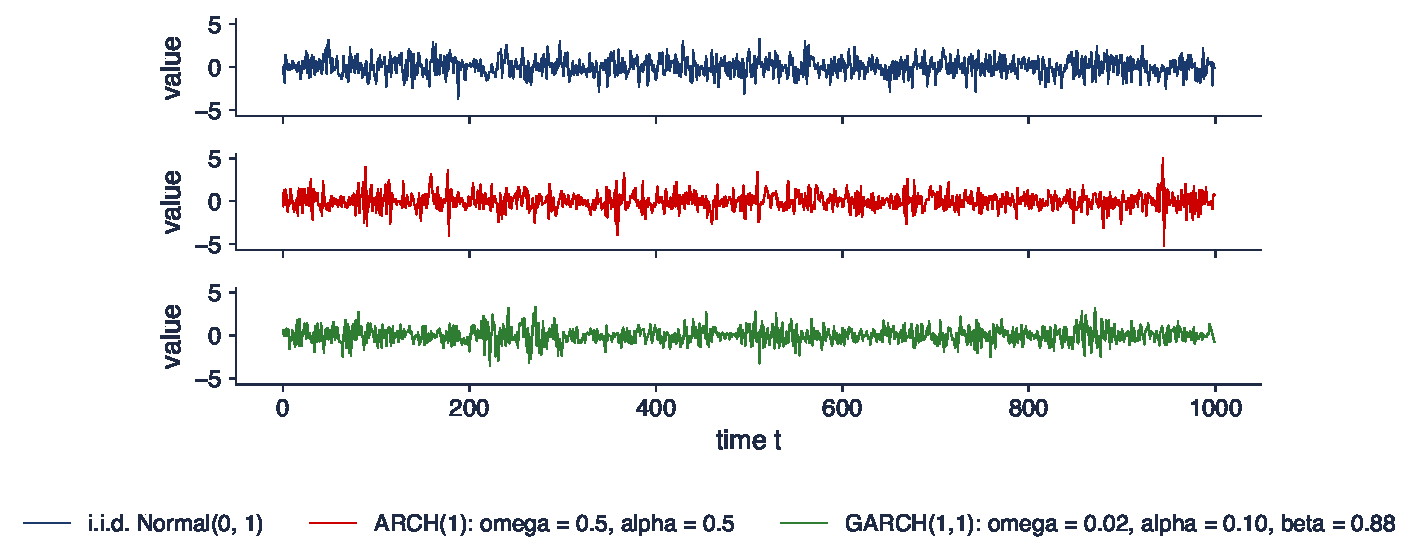
\includegraphics[width=0.97\textwidth,height=0.46\textheight,keepaspectratio]{tsa_ch5_simulated.pdf}
\end{center}
\vspace{-0.25cm}
\begin{itemize}
    \item Three series of 1000 values with unconditional variance 1: i.i.d.\ Normal; ARCH(1) with $\omega = \alpha = 0.5$; GARCH(1,1) with $\omega = 0.02$, $\alpha = 0.10$, $\beta = 0.88$ (next section)
    \item Sample kurtosis: i.i.d.\ $3.12$, ARCH $4.91$, GARCH $3.74$ (theory: 3, $9.0$, $6.06$): the fourth moment converges slowly
    \item Interpretation: ARCH(1) gives isolated spikes; GARCH(1,1) gives long calm and long agitated periods, as in real returns
\end{itemize}
\quantlet{TSA\_ch5\_simulation\_likelihood}{\qlurl{TSA_ch5_simulation_likelihood}}
\end{frame}

\begin{frame}{ARCH($q$) and its limits}
\itemsize{\footnotesize}
\begin{itemize}
    \item \textbf{ARCH($q$)}: $\sigma_t^2 = \omega + \alpha_1\varepsilon_{t-1}^2 + \dots + \alpha_q\varepsilon_{t-q}^2$, $\alpha_i \ge 0$; stationary if $\sum_i \alpha_i < 1$
    \begin{itemize}
        \item a shock affects the variance for exactly $q$ days; real clustering lasts for months
    \end{itemize}
\end{itemize}\begin{center}
\footnotesize
\begin{tabular}{lrrrrr}
\toprule
S\&P 500, Normal $z_t$ & parameters & log-likelihood & AIC & BIC & $\sum\alpha_i$ (+$\beta$) \\
\midrule
ARCH(1) & 3 & $-10305.5$ & 20617.0 & 20637.5 & $0.394$ \\
ARCH(5) & 7 & $-9340.5$ & 18695.1 & 18742.7 & $0.816$ \\
ARCH(10) & 12 & $-9227.6$ & 18479.3 & 18561.0 & $0.849$ \\
GARCH(1,1) & 4 & $-9218.0$ & \textbf{18444.0} & \textbf{18471.2} & $0.980$ \\
\bottomrule
\end{tabular}
\end{center}
\begin{itemize}
    \item AIC (Akaike) and BIC (Bayesian information criterion): $-2\ell + $ penalty for parameters (\tsachlink{https://danpele.github.io/Time-Series-Analysis/EN/Courses/chapter2_arma_models.pdf}{Chapter 2}); smaller is better
    \item Interpretation: ARCH needs ten lags and still loses to GARCH(1,1), which has four parameters: the motivation for GARCH
\end{itemize}\quantlet{TSA\_ch5\_garch\_estimation}{\qlurl{TSA_ch5_garch_estimation}}
\end{frame}

\begin{frame}{Recap: the ARCH model}
\itemsize{\small}
\begin{itemize}
    \item $\sigma_t^2 = \omega + \sum_i\alpha_i\varepsilon_{t-i}^2$: an AR model for the squared shocks
    \item Unconditional variance $\omega/(1 - \sum\alpha_i)$; kurtosis above 3 even with Normal innovations
    \item Real clustering needs many lags: GARCH replaces them with one extra parameter
\end{itemize}
\end{frame}


%=============================================================================
\section{The GARCH(1,1) model}
%=============================================================================

\begin{frame}{1986: Tim Bollerslev and GARCH}
\itemsize{\small}
\begin{columns}[T]
\begin{column}{0.56\textwidth}
\begin{itemize}
    \item \refBoll, a doctoral student of Engle at the University of California, San Diego: add yesterday's variance to the equation
    \begin{itemize}
        \item \textbf{GARCH} (generalised ARCH): a few parameters replace a long ARCH($q$)
    \end{itemize}
    \item Student-t innovations for returns: \refBollT
    \item Still the benchmark: \refHL\ compared 330 volatility models and found GARCH(1,1) hard to beat on exchange rates
\end{itemize}
\end{column}
\begin{column}{0.40\textwidth}
\centering
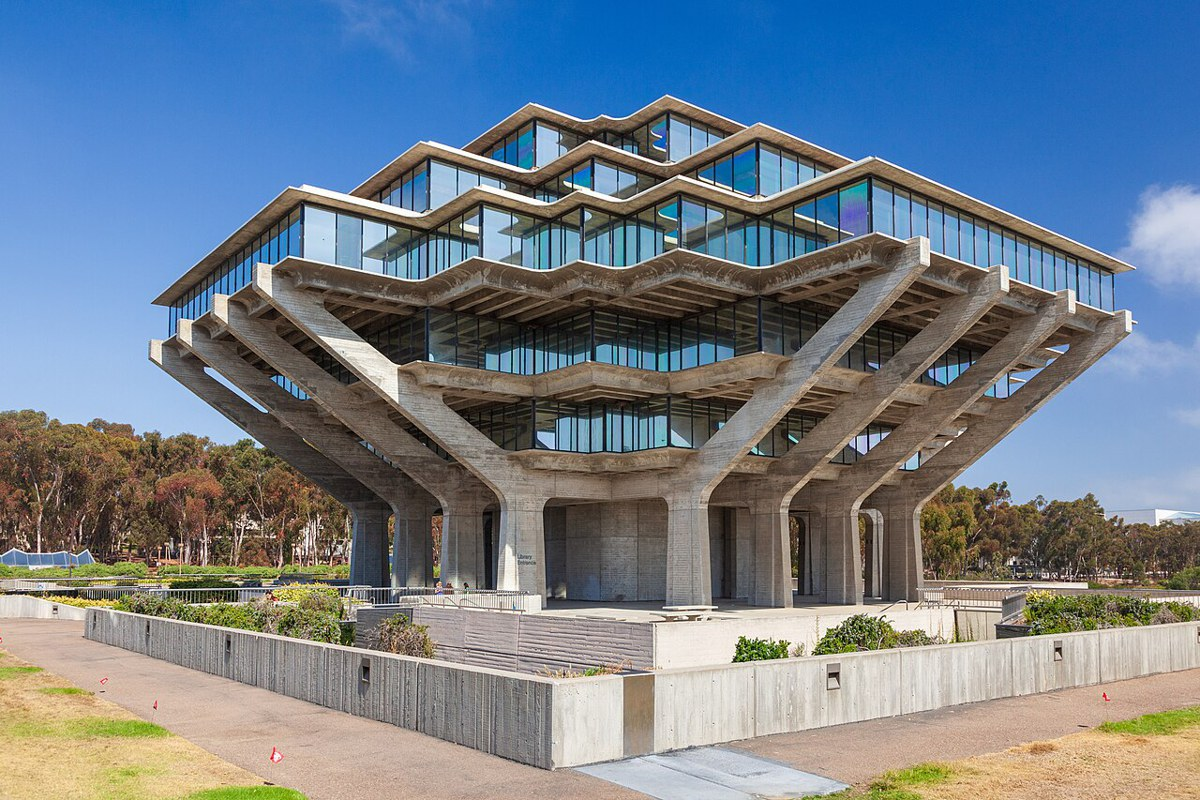
\includegraphics[height=0.36\textheight]{ch5_ucsd_geisel_2010.jpg}\\[1mm]
\imgcap{Geisel Library, University of California, San Diego}
\imgcredit{https://commons.wikimedia.org/wiki/File:Geisel_Library,_UC_San_Diego.jpg}{Photo: Stephen Bay (2010); CC BY 4.0; Wikimedia Commons}
\end{column}
\end{columns}
\end{frame}

\begin{frame}{GARCH(1,1): definition}
\itemsize{\small}
\begin{itemize}
    \item $\varepsilon_t = \sigma_t z_t$, \quad $\sigma_t^2 = \omega + \alpha\,\varepsilon_{t-1}^2 + \beta\,\sigma_{t-1}^2$, \quad $\omega > 0$, $\alpha \ge 0$, $\beta \ge 0$
    \begin{itemize}
        \item GARCH($p$,$q$) adds more lags of both kinds; in practice (1,1) is almost always enough
    \end{itemize}
    \item Reading the parameters
    \begin{itemize}
        \item $\alpha$: the \textbf{reaction} to yesterday's news; $\beta$: the \textbf{memory} of the variance
        \item $\alpha + \beta$: the \textbf{persistence}; $\omega$ sets the long-run level
    \end{itemize}
    \item By recursion: an ARCH($\infty$) with geometric weights
    \begin{itemize}
        \item $\sigma_t^2 = \dfrac{\omega}{1 - \beta} + \alpha\sum_{j=0}^{\infty}\beta^j\,\varepsilon_{t-1-j}^2$: all past shocks matter, with weights that decay like $\beta^j$
    \end{itemize}
\end{itemize}
\end{frame}

\begin{frame}{GARCH(1,1) as an ARMA(1,1) for the squared shocks}
\itemsize{\small}
\begin{itemize}
    \item As for ARCH, write $\varepsilon_t^2 = \sigma_t^2 + v_t$ and substitute $\sigma_t^2 = \varepsilon_t^2 - v_t$ in the equation
    \begin{itemize}
        \item $\varepsilon_t^2 = \omega + (\alpha + \beta)\,\varepsilon_{t-1}^2 + v_t - \beta\,v_{t-1}$
        \item an ARMA(1,1) (\tsachlink{https://danpele.github.io/Time-Series-Analysis/EN/Courses/chapter2_arma_models.pdf}{Chapter 2}) with AR coefficient $\alpha + \beta$ and MA coefficient $-\beta$
    \end{itemize}
    \item Consequences
    \begin{itemize}
        \item \textbf{covariance stationary} if $\alpha + \beta < 1$ (the AR root outside the unit circle)
        \item the ACF of $\varepsilon_t^2$ decays like $(\alpha + \beta)^k$: slow when the persistence is close to 1, as in the ACF of real squared returns
        \item identification by the ACF and the PACF (partial autocorrelation function) of $\varepsilon_t^2$ is possible in principle, but in practice we use MLE (Section 5)
    \end{itemize}
\end{itemize}
\end{frame}

\begin{frame}{Long-run variance, kurtosis, persistence and half-life}
\itemsize{\small}
\begin{itemize}
    \item \textbf{Long-run (unconditional) variance}: $\bar\sigma^2 = \omega/(1 - \alpha - \beta)$; annualised volatility $\sqrt{252\,\bar\sigma^2}$ for 252 trading days
    \begin{itemize}
        \item kurtosis with Normal $z_t$: $K = 3\,\dfrac{1 - (\alpha + \beta)^2}{1 - (\alpha + \beta)^2 - 2\alpha^2} > 3$; $\alpha = 0.10$, $\beta = 0.88$: $K = 6.06$
    \end{itemize}
    \item A deviation from $\bar\sigma^2$ shrinks by the factor $\alpha + \beta$ each day (Section 9): $E_t[\sigma_{t+h}^2] - \bar\sigma^2 = (\alpha + \beta)^{h-1}(\sigma_{t+1}^2 - \bar\sigma^2)$
    \begin{itemize}
        \item \textbf{half-life}: the number of days after which half of a variance shock is gone, $h_{1/2} = \ln 0.5/\ln(\alpha + \beta)$
        \item $\alpha + \beta = 0.90$: 6.6 days; $0.98$: 34.3 days; $0.99$: 69.0 days: small changes near 1 matter a lot
    \end{itemize}
\end{itemize}
\end{frame}

\begin{frame}{Worked example: one GARCH(1,1) step}
\itemsize{\small}
\begin{itemize}
    \item Daily returns in \%: $\omega = 0.02$, $\alpha = 0.10$, $\beta = 0.88$, $\mu = 0$
    \item Long-run quantities
    \begin{itemize}
        \item persistence $\alpha + \beta = 0.98$; $\bar\sigma^2 = 0.02/(1 - 0.98) = 1.00$; annualised volatility $\sqrt{252 \times 1.00} = 15.9\%$
        \item half-life $\ln 0.5/\ln 0.98 = 34.3$ days
    \end{itemize}
    \item Today: $\sigma_t^2 = 1.2$ and the return is $r_t = -3\%$
    \begin{itemize}
        \item tomorrow: $\sigma_{t+1}^2 = 0.02 + 0.10 \times 9 + 0.88 \times 1.2 = 1.976$, $\sigma_{t+1} = 1.41\%$
        \item the shock raised the variance from 1.2 to almost 2; it then decays towards 1.00 with the factor 0.98 per day
    \end{itemize}
\end{itemize}
\end{frame}

\begin{frame}{IGARCH and the link with EWMA}
\itemsize{\small}
\begin{itemize}
    \item \textbf{IGARCH} (integrated GARCH) \refEB: $\alpha + \beta = 1$: a unit root in the ARMA(1,1) for $\varepsilon_t^2$ (\tsachlink{https://danpele.github.io/Time-Series-Analysis/EN/Courses/chapter3_unit_roots_arima_models.pdf}{Chapter 3})
    \begin{itemize}
        \item shocks to the variance never die out: no half-life, no finite unconditional variance
    \end{itemize}
    \item \textbf{EWMA} (exponentially weighted moving average) of \refRM: $\sigma_t^2 = \lambda\sigma_{t-1}^2 + (1 - \lambda)r_{t-1}^2$
    \begin{itemize}
        \item simple exponential smoothing (\tsachlink{https://danpele.github.io/Time-Series-Analysis/EN/Courses/chapter0_introduction.pdf}{Chapter 0}) applied to $r_t^2$, with smoothing constant $1 - \lambda$
        \item an IGARCH with $\omega = 0$, $\alpha = 1 - \lambda$, $\beta = \lambda$; RiskMetrics uses $\lambda = 0.94$ for daily data (half-life of the weights 11.2 days)
    \end{itemize}
    \item \textbf{Question for the room}: right after a crash, an analyst forecasts the volatility one year ahead with EWMA. What goes wrong?
    \begin{itemize}
        \item \textbf{Answer}: EWMA keeps today's crisis level for the whole year; GARCH lets it decay towards the long-run level
    \end{itemize}
\end{itemize}
\end{frame}

\begin{frame}{GARCH, EWMA and a rolling window in 2020}
\itemsize{\footnotesize}
\begin{center}
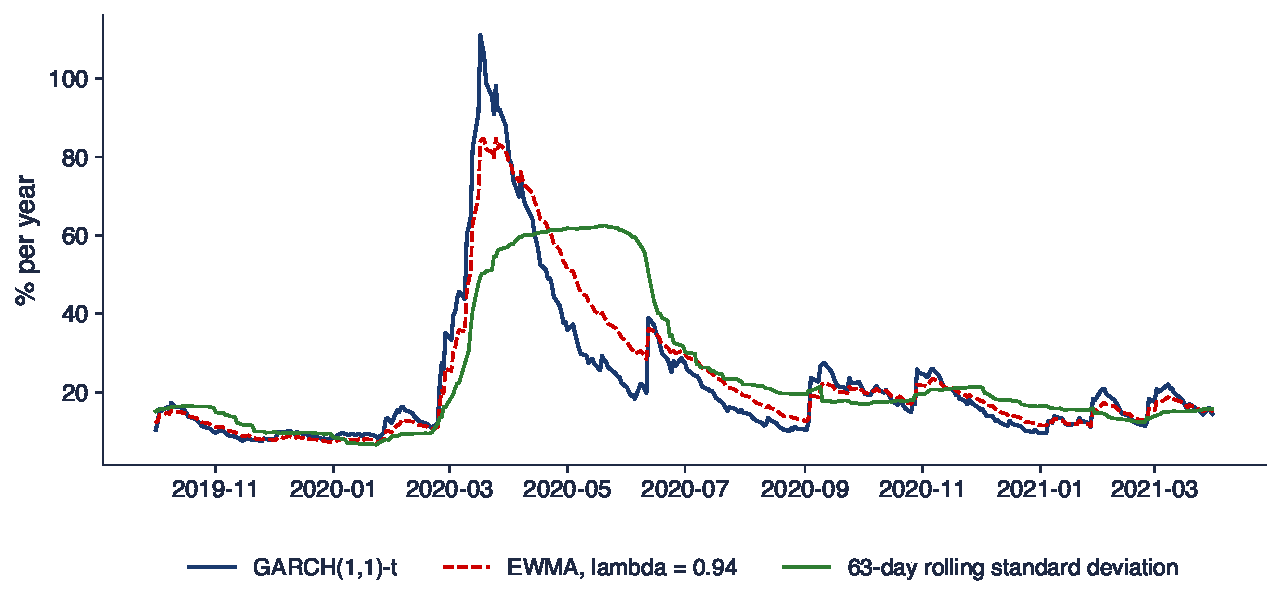
\includegraphics[width=0.97\textwidth,height=0.52\textheight,keepaspectratio]{tsa_ch5_ewma_garch.pdf}
\end{center}
\vspace{-0.25cm}
\begin{itemize}
    \item S\&P 500, annualised volatility: GARCH(1,1)-t estimated on all data, EWMA with $\lambda = 0.94$, and the standard deviation of the last 63 days (\tsachlink{https://danpele.github.io/Time-Series-Analysis/EN/Courses/chapter0_introduction.pdf}{Chapter 0}: a moving average)
\end{itemize}
\quantlet{TSA\_ch5\_volatility\_markets}{\qlurl{TSA_ch5_volatility_markets}}
\end{frame}

\begin{frame}{Interpreting the three estimates}
\itemsize{\small}
\begin{itemize}
    \item Peaks: GARCH 111\% (17 March 2020), EWMA 85\% (25 March 2020), 63-day window 63\% (20 May 2020)
    \item The rolling window reacts late and falls abruptly when the crash leaves the window (the ``ghost'' of the crash)
    \begin{itemize}
        \item on 30 June 2020: GARCH 28\%, EWMA 30\%, window 32\%
    \end{itemize}
    \item GARCH reacts fastest ($\alpha$ larger than $1 - \lambda$) and decays fastest (mean reversion); EWMA lies in between
\end{itemize}
\end{frame}

\begin{frame}{Recap: the GARCH(1,1) model}
\itemsize{\small}
\begin{itemize}
    \item $\sigma_t^2 = \omega + \alpha\varepsilon_{t-1}^2 + \beta\sigma_{t-1}^2$: reaction $\alpha$, memory $\beta$; an ARMA(1,1) for $\varepsilon_t^2$
    \item $\alpha + \beta < 1$: long-run variance $\omega/(1 - \alpha - \beta)$, half-life $\ln 0.5/\ln(\alpha + \beta)$
    \item $\alpha + \beta = 1$: IGARCH; EWMA is an IGARCH without $\omega$
\end{itemize}
\end{frame}


%=============================================================================
\section{Estimation by maximum likelihood}
%=============================================================================

\begin{frame}{The likelihood of a GARCH model}
\itemsize{\small}
\begin{itemize}
    \item The returns are dependent, so the joint density is a product of conditional densities
    \begin{itemize}
        \item $f(r_1, \dots, r_T) = f(r_1)\prod_{t=2}^{T} f(r_t \mid \mathcal{F}_{t-1})$, with $r_t \mid \mathcal{F}_{t-1} \sim N(\mu, \sigma_t^2)$ for Normal innovations
    \end{itemize}
    \item \textbf{Conditional log-likelihood}, $\theta = (\mu, \omega, \alpha, \beta)$:
    \begin{itemize}
        \item $\ell(\theta) = -\dfrac12\sum_{t=2}^{T}\Big[\ln(2\pi) + \ln\sigma_t^2(\theta) + \dfrac{(r_t - \mu)^2}{\sigma_t^2(\theta)}\Big]$
        \item $\sigma_t^2(\theta)$ is computed recursively from a starting value $\sigma_1^2$ (for example the sample variance)
    \end{itemize}
    \item \textbf{MLE} (maximum likelihood estimation): $\hat\theta = \arg\max_\theta \ell(\theta)$, under $\omega > 0$, $\alpha, \beta \ge 0$, $\alpha + \beta < 1$
    \begin{itemize}
        \item no closed form: a numerical optimiser searches for the maximum; OLS is not possible, since $\sigma_t^2$ is not observed
    \end{itemize}
\end{itemize}
\end{frame}

\begin{frame}{The likelihood of ARCH(1)}
\itemsize{\footnotesize}
\begin{center}
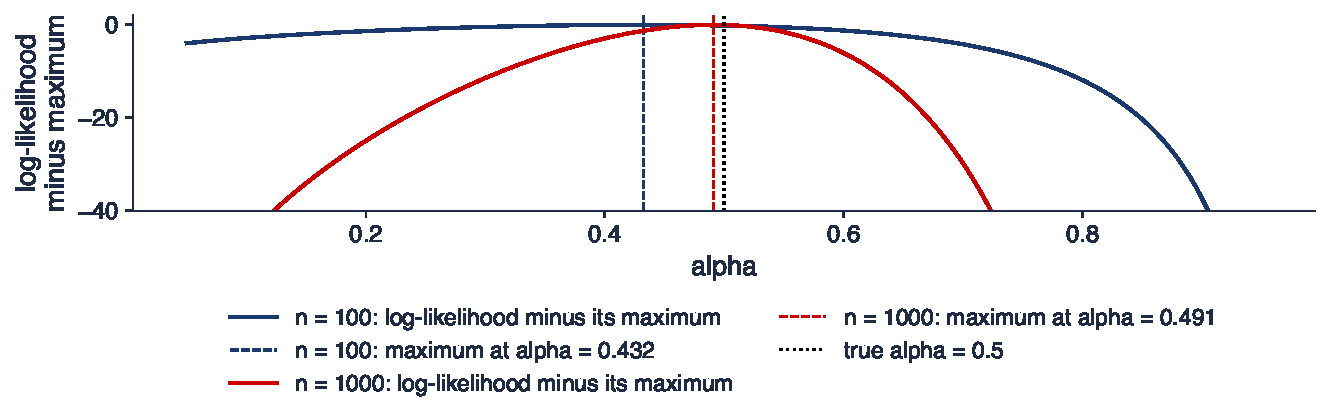
\includegraphics[width=0.97\textwidth,height=0.48\textheight,keepaspectratio]{tsa_ch5_lik_arch1.pdf}
\end{center}
\vspace{-0.25cm}
\begin{itemize}
    \item Simulated ARCH(1) with $\omega = \alpha = 0.5$; $\ell(\alpha)$ with $\omega = 1 - \alpha$; each curve minus its maximum
    \item $n = 100$: $\hat\alpha = 0.432$ (standard error $0.127$); $n = 1000$: $\hat\alpha = 0.491$ ($0.035$)
    \item Interpretation: more data make the curve sharper; its curvature at the maximum gives the standard error
\end{itemize}
\quantlet{TSA\_ch5\_simulation\_likelihood}{\qlurl{TSA_ch5_simulation_likelihood}}
\end{frame}

\begin{frame}{The likelihood of GARCH(1,1)}
\itemsize{\footnotesize}
\begin{center}
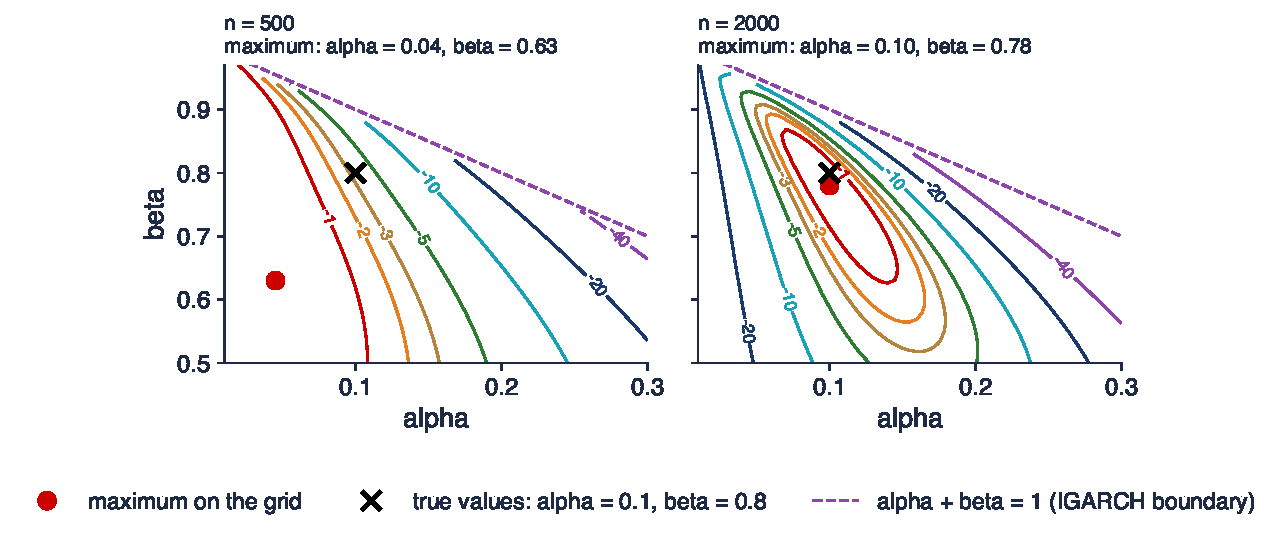
\includegraphics[width=0.97\textwidth,height=0.46\textheight,keepaspectratio]{tsa_ch5_lik_garch.pdf}
\end{center}
\vspace{-0.25cm}
\begin{itemize}
    \item Simulated GARCH(1,1) with $\omega = 0.1$, $\alpha = 0.1$, $\beta = 0.8$; $\omega$ set so that the unconditional variance equals the sample variance; contours: log-likelihood minus its maximum
    \item $n = 500$: maximum at $(0.04, 0.63)$, far from the truth; $n = 2000$: $(0.10, 0.78)$
    \item Interpretation: a long, flat ridge along which $\alpha$ and $\beta$ trade off: GARCH needs long samples
\end{itemize}
\quantlet{TSA\_ch5\_simulation\_likelihood}{\qlurl{TSA_ch5_simulation_likelihood}}
\end{frame}

\begin{frame}{Estimation step by step and with the \texttt{arch} package}
\itemsize{\footnotesize}
\begin{center}
\footnotesize
\begin{tabular}{lrrrr}
\toprule
S\&P 500, GARCH(1,1)-N & step by step (SE) & \texttt{arch} & classic SE & robust SE \\
\midrule
$\mu$ & $0.0614$ ($0.0098$) & $0.0615$ & $0.0098$ & $0.0100$ \\
$\omega$ & $0.0253$ ($0.0030$) & $0.0254$ & $0.0030$ & $0.0048$ \\
$\alpha$ & $0.1205$ ($0.0086$) & $0.1206$ & $0.0086$ & $0.0118$ \\
$\beta$ & $0.8600$ ($0.0091$) & $0.8599$ & $0.0091$ & $0.0125$ \\
\bottomrule
\end{tabular}
\end{center}
\begin{itemize}
    \item Step by step: $-\ell(\theta)$ written in Python and minimised with \texttt{scipy.optimize.minimize} under $\alpha + \beta < 1$
    \begin{itemize}
        \item with the package: \texttt{arch\_model(r, mean='Constant', vol='GARCH', p=1, q=1, dist='normal').fit()}
    \end{itemize}
    \item SE (standard error), classic: from the inverse Hessian (the curvature of $\ell$); robust: valid when $z_t$ is not Normal \refBW
    \item Interpretation: same estimates by both routes; the robust SE are about 1.4 times larger: with heavy-tailed $z_t$ the classic SE overstate the precision
\end{itemize}\quantlet{TSA\_ch5\_garch\_estimation}{\qlurl{TSA_ch5_garch_estimation}}
\end{frame}

\begin{frame}{Quasi-maximum likelihood and practical rules}
\itemsize{\small}
\begin{itemize}
    \item \textbf{QMLE} (quasi-maximum likelihood estimation): maximise the Normal likelihood even if $z_t$ is not Normal
    \begin{itemize}
        \item the estimates stay consistent if $\mu_t$ and $\sigma_t^2$ are correctly specified, but only the robust (``sandwich'') SE are valid \refBW
    \end{itemize}
    \item Practical rules
    \begin{itemize}
        \item returns in \% (not decimals): the optimiser fails when $\omega$ is tiny; \texttt{arch} warns about badly scaled data
        \item EUR/RON moves about 0.3\% a day: we estimate on $10\,r_t$ and convert $\omega$ back (divide by 100)
        \item use at least 1000--2000 daily observations; check the convergence flag of the optimiser
        \item an estimate on the boundary ($\hat\alpha + \hat\beta = 1$ or $\hat\alpha = 0$) has no usual standard error: report it as such
    \end{itemize}
\end{itemize}
\end{frame}

\begin{frame}{Student-t and skewed-t innovations}
\itemsize{\small}
\begin{itemize}
    \item GARCH with Normal $z_t$ explains only part of the kurtosis: S\&P 500 returns $13.7$, standardised residuals $\hat z_t = \hat\varepsilon_t/\hat\sigma_t$ still $4.7$
    \begin{itemize}
        \item the remaining heavy tails must come from the distribution of $z_t$
    \end{itemize}
    \item \textbf{Standardised Student-t} with $\nu > 2$ degrees of freedom \refBollT
    \begin{itemize}
        \item $z_t = t_\nu\sqrt{(\nu - 2)/\nu}$ has variance 1; kurtosis $3 + 6/(\nu - 4)$ for $\nu > 4$; $\nu \to \infty$: the Normal distribution
        \item $\nu$ is estimated together with $(\mu, \omega, \alpha, \beta)$: \texttt{dist='t'} in \texttt{arch}
    \end{itemize}
    \item \textbf{Skewed t} \refHansen: one more parameter $\lambda \in (-1, 1)$; $\lambda < 0$: a longer left tail (\texttt{dist='skewt'})
    \begin{itemize}
        \item nested models: Normal $\subset$ t $\subset$ skewed t; compare them with LR (likelihood ratio) tests or AIC/BIC
    \end{itemize}
\end{itemize}
\end{frame}

\begin{frame}{S\&P 500: three innovation distributions}
\itemsize{\footnotesize}
\begin{center}
\footnotesize
\begin{tabular}{lrrrrrrr}
\toprule
GARCH(1,1) & $\omega$ & $\alpha$ & $\beta$ & $\nu$ & $\lambda$ & log-lik. & $\alpha + \beta$ \\
\midrule
Normal & $0.0254$ & $0.121$ & $0.860$ & -- & -- & $-9218.0$ & $0.980$ \\
Student-t & $0.0157$ & $0.123$ & $0.872$ & $6.26$ & -- & $-9062.5$ & $0.995$ \\
skewed t & $0.0153$ & $0.120$ & $0.872$ & $6.92$ & $-0.114$ & $-9038.4$ & $0.993$ \\
\bottomrule
\end{tabular}
\end{center}
\begin{itemize}
    \item LR statistic $2(\ell_1 - \ell_0)$: t against Normal $311.0$ (1 restriction, $\chi^2_{0.95}(1) = 3.84$); skewed t against t $48.1$: both reject the smaller model
    \item $\hat\nu = 6.26$: tails far heavier than Normal; $\hat\lambda = -0.114$: large falls more frequent than large rises
    \item Interpretation: $\alpha$ and $\beta$ hardly change; the innovation distribution matters for tail quantiles (VaR), less for $\sigma_t$
\end{itemize}\quantlet{TSA\_ch5\_garch\_estimation}{\qlurl{TSA_ch5_garch_estimation}}
\end{frame}

\begin{frame}{QQ plots of the standardised residuals}
\itemsize{\footnotesize}
\begin{center}
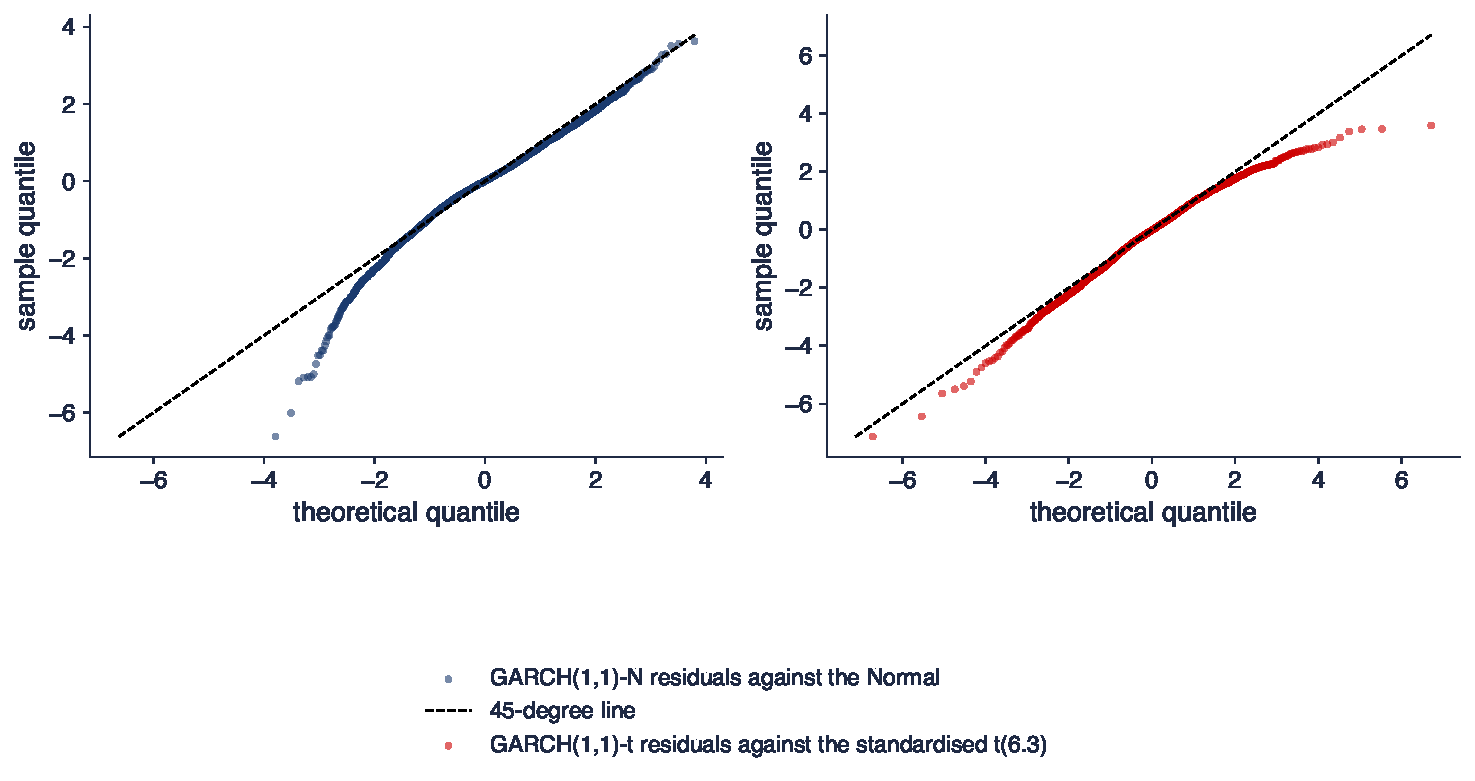
\includegraphics[width=0.97\textwidth,height=0.46\textheight,keepaspectratio]{tsa_ch5_qq.pdf}
\end{center}
\vspace{-0.25cm}
\begin{itemize}
    \item QQ (quantile--quantile) plot: sample quantiles of $\hat z_t$ against the quantiles of the assumed distribution; a straight line means a good fit
    \item Left, GARCH-N against the Normal: 0.1\% quantile $-4.81$, against $-3.09$ in theory; right, GARCH-t against the standardised t ($\hat\nu = 6.3$): $-4.79$ against $-4.19$
    \item Interpretation: the t fits much better, but the largest falls are still deeper: the left tail is the problem (asymmetry, Section 7)
\end{itemize}
\quantlet{TSA\_ch5\_garch\_estimation}{\qlurl{TSA_ch5_garch_estimation}}
\end{frame}

\begin{frame}{Recap: estimation by maximum likelihood}
\itemsize{\small}
\begin{itemize}
    \item $\ell(\theta)$ = sum of conditional log-densities; $\sigma_t^2(\theta)$ computed recursively; numerical maximisation
    \item The likelihood has a ridge in $(\alpha, \beta)$: long samples; report robust SE
    \item Student-t or skewed-t innovations for the remaining heavy tails
\end{itemize}
\end{frame}


%=============================================================================
\section{GARCH in four markets and ARMA-GARCH models}
%=============================================================================

\begin{frame}{GARCH(1,1)-t estimates}
\itemsize{\footnotesize}
\begin{center}
\scriptsize
\begin{tabular}{lrrrrrrrrr}
\toprule
& from & $\omega$ & $\alpha$ & $\beta$ & $\nu$ & $\alpha + \beta$ & half-life & long-run vol. & sample vol. \\
\midrule
S\&P 500 & 2000 & $0.0157$ & $0.123$ & $0.872$ & $6.26$ & $0.995$ & 131 & 27.3 & 19.2 \\
BET & 2000 & $0.0448$ & $0.192$ & $0.799$ & $5.01$ & $0.991$ & 74 & 34.7 & 22.1 \\
EUR/RON & 2005 & $0.0000$ & $0.123$ & $0.877$ & $4.20$ & $1.000$ & -- & -- & 4.4 \\
Bitcoin & 2014 & $0.1937$ & $0.109$ & $0.891$ & $3.18$ & $1.000$ & -- & -- & 66.6 \\
\bottomrule
\end{tabular}
\end{center}
\begin{itemize}
    \item Daily log returns in \% to 18 September 2026; half-life in days; volatilities annualised with the actual number of observations per year (Bitcoin: 365), in \%
    \item S\&P 500 and BET: $\alpha + \beta$ 0.995 and 0.991, half-lives of 131 and 74 trading days; BET reacts more to news ($\alpha = 0.192$)
    \item EUR/RON and Bitcoin: $\hat\alpha + \hat\beta = 1$ on the boundary: IGARCH; every $\hat\nu$ between 3.18 and 6.26: heavy tails everywhere
\end{itemize}\quantlet{TSA\_ch5\_volatility\_markets}{\qlurl{TSA_ch5_volatility_markets}}
\end{frame}

\begin{frame}{Interpreting IGARCH and the long-run volatility}
\itemsize{\small}
\begin{itemize}
    \item EUR/RON: $\hat\omega \approx 0$ and $\hat\beta = 0.88$: an EWMA with $\lambda \approx 0.88$; Bitcoin: $\hat\beta = 0.89$
    \begin{itemize}
        \item no half-life and no long-run volatility: the volatility level drifts like a random walk (\tsachlink{https://danpele.github.io/Time-Series-Analysis/EN/Courses/chapter3_unit_roots_arima_models.pdf}{Chapter 3})
        \item EUR/RON: a managed rate whose volatility fell from one regime to the next (the BNR policy changes over time)
    \end{itemize}
    \item \textbf{Question for the room}: S\&P 500: long-run volatility 27.3\%, sample volatility 19.2\%. Is the model wrong?
    \begin{itemize}
        \item \textbf{Answer}: not necessarily: $\bar\sigma^2 = \omega/(1 - \alpha - \beta)$ divides by $1 - \alpha - \beta = 0.0053$, a small and imprecise number
        \item the Normal GARCH gives 18.1\%: the long-run level is the least reliable output of a persistent GARCH
    \end{itemize}
\end{itemize}
\end{frame}

\begin{frame}{Conditional volatility: S\&P 500 and BET}
\itemsize{\footnotesize}
\begin{center}
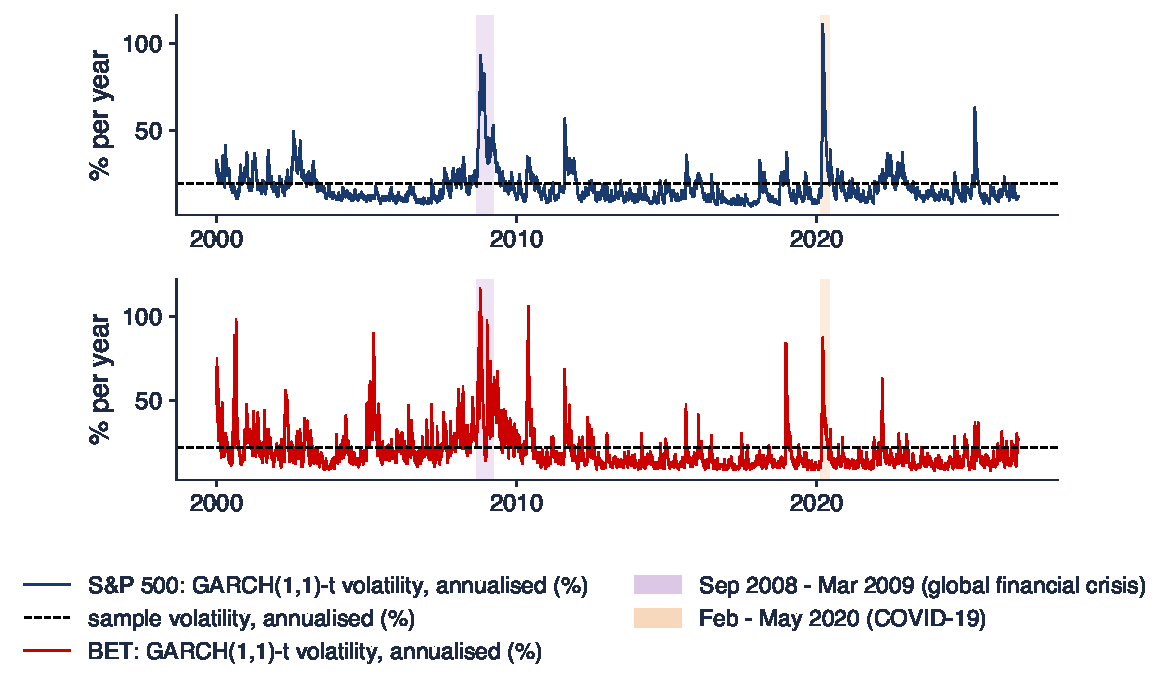
\includegraphics[width=0.97\textwidth,height=0.54\textheight,keepaspectratio]{tsa_ch5_vol_sp500_bet.pdf}
\end{center}
\vspace{-0.25cm}
\begin{itemize}
    \item GARCH(1,1)-t volatility $\hat\sigma_t$, annualised; dashed: the sample volatility
    \item S\&P 500: peaks 93\% (16 October 2008) and 111\% (17 March 2020); BET: 117\% (15 October 2008) and 88\% (18 March 2020); medians 14.3\% and 15.6\%
\end{itemize}
\quantlet{TSA\_ch5\_volatility\_markets}{\qlurl{TSA_ch5_volatility_markets}}
\end{frame}

\begin{frame}{Conditional volatility: EUR/RON and Bitcoin}
\itemsize{\footnotesize}
\begin{center}
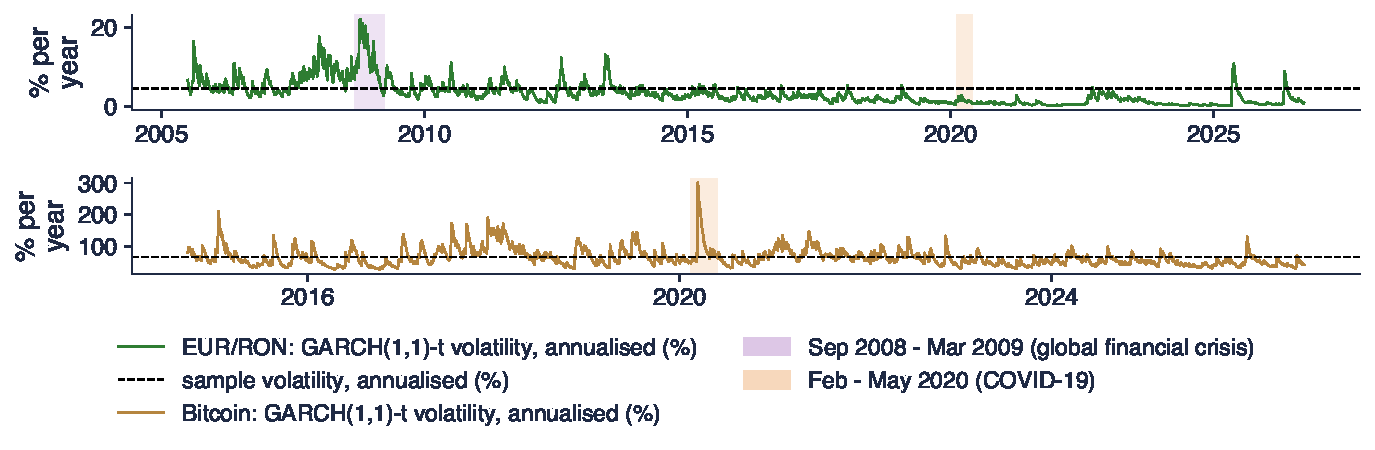
\includegraphics[width=0.97\textwidth,height=0.52\textheight,keepaspectratio]{tsa_ch5_vol_eurron_btc.pdf}
\end{center}
\vspace{-0.25cm}
\begin{itemize}
    \item EUR/RON: 22\% at the peak of the 2008 crisis (13 October 2008), only 3\% in 2020; on 18 September 2026: 1.0\%
    \item Bitcoin: 301\% on 13 March 2020; median 58.7\%, 4.1 times the median of the S\&P 500
    \item Interpretation: the two IGARCH series have volatility levels that wander: no single ``normal'' level
\end{itemize}
\quantlet{TSA\_ch5\_volatility\_markets}{\qlurl{TSA_ch5_volatility_markets}}
\end{frame}

\begin{frame}{How long does a volatility shock last?}
\itemsize{\footnotesize}
\begin{center}
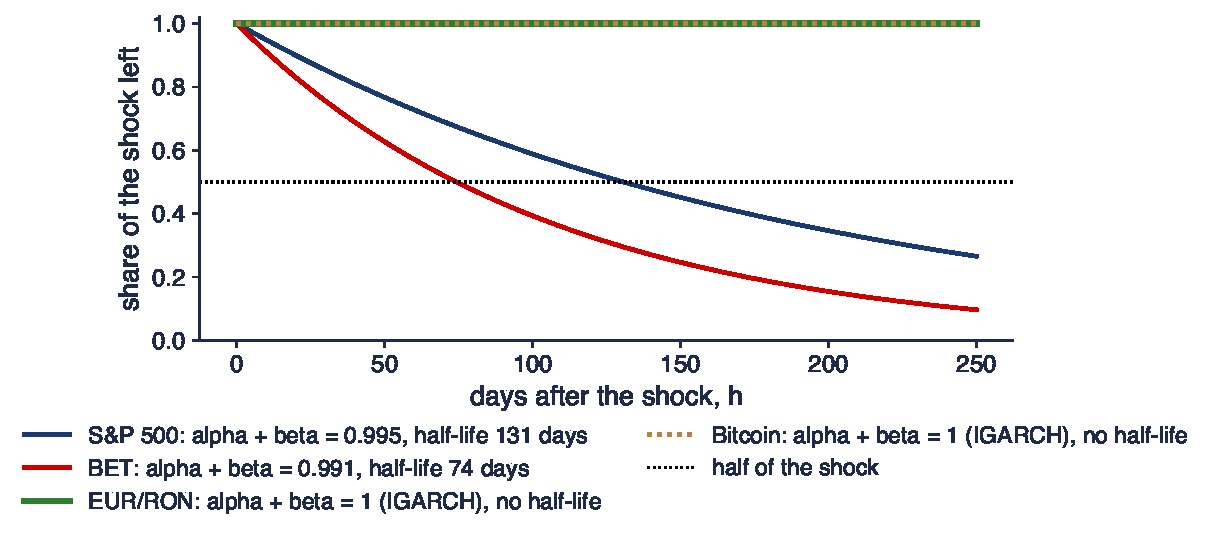
\includegraphics[width=0.97\textwidth,height=0.50\textheight,keepaspectratio]{tsa_ch5_persistence.pdf}
\end{center}
\vspace{-0.25cm}
\begin{itemize}
    \item Share of a variance shock left after $h$ days: $(\alpha + \beta)^h$; the half-life is where the curve crosses 1/2
    \item Interpretation: after a crisis the S\&P 500 needs about half a year to halve the excess variance, the BET about three months; EUR/RON and Bitcoin never
\end{itemize}
\quantlet{TSA\_ch5\_volatility\_markets}{\qlurl{TSA_ch5_volatility_markets}}
\end{frame}

\begin{frame}{ARMA-GARCH: one model for the mean and the variance}
\itemsize{\small}
\begin{itemize}
    \item \textbf{ARMA($p$,$q$)-GARCH(1,1)}: $r_t = c + \sum_{i=1}^{p}\phi_i r_{t-i} + \varepsilon_t + \sum_{j=1}^{q}\theta_j\varepsilon_{t-j}$, \quad $\varepsilon_t = \sigma_t z_t$, \quad $\sigma_t^2 = \omega + \alpha\varepsilon_{t-1}^2 + \beta\sigma_{t-1}^2$
    \begin{itemize}
        \item the ARMA part is the model of \tsachlink{https://danpele.github.io/Time-Series-Analysis/EN/Courses/chapter2_arma_models.pdf}{Chapter 2}; its errors are no longer i.i.d., they follow a GARCH
    \end{itemize}
    \item Estimation: both parts at once, by maximum likelihood
    \begin{itemize}
        \item in \texttt{arch}: \texttt{arch\_model(r, mean='AR', lags=1, vol='GARCH', dist='t')} (AR means only; for MA terms use two steps or another package)
    \end{itemize}
    \item Why not OLS for the mean and then GARCH?
    \begin{itemize}
        \item the OLS coefficients are still consistent, but their usual SE assume a constant variance: the $t$ tests of \tsachlink{https://danpele.github.io/Time-Series-Analysis/EN/Courses/chapter2_arma_models.pdf}{Chapter 2} are wrong
        \item the joint maximum likelihood estimate gives less weight to stormy days, hence more precise $\hat\phi$ and valid intervals
    \end{itemize}
\end{itemize}
\end{frame}

\begin{frame}{AR(1)-GARCH(1,1)-t on four series}
\itemsize{\footnotesize}
\begin{center}
\scriptsize
\begin{tabular}{lrrrrrr}
\toprule
& $p$ (BIC) & $\hat\phi$, OLS (SE) & $\hat\phi$, AR-GARCH (SE) & $Q(10)$ of $\hat z_t$, const. mean & $Q(10)$ of $\hat z_t$, AR(1) & $\Delta$BIC \\
\midrule
S\&P 500 & 1 & $-0.099$ ($0.012$) & $-0.054$ ($0.012$) & $21.9$ (0.016) & $15.1$ (0.087) & ${-19.5}$ \\
BET & 1 & $0.109$ ($0.012$) & $0.091$ ($0.013$) & $114.6$ ($<$\,0.001) & $28.6$ ($<$\,0.001) & ${-46.9}$ \\
EUR/RON & 3 & $0.170$ ($0.013$) & $0.031$ ($0.016$) & $10.5$ (0.402) & $8.7$ (0.469) & ${4.2}$ \\
Bitcoin & 0 & $-0.022$ ($0.015$) & $-0.043$ ($0.014$) & $29.9$ ($<$\,0.001) & $48.4$ ($<$\,0.001) & ${-9.5}$ \\
\bottomrule
\end{tabular}
\end{center}
\begin{itemize}
    \item $p$: AR order chosen by BIC with a constant variance; SE of the AR-GARCH: robust; $\Delta$BIC: AR(1)-GARCH-t minus GARCH-t with a constant mean (negative: AR(1) preferred)
    \item S\&P 500: $\hat\phi$ shrinks from -0.099 to -0.054: the OLS value is driven by the stormy days of 2008 and 2020
    \item BET: a positive autocorrelation survives ($\hat\phi = 0.091$, $t = 6.8$): slow price adjustment in a less liquid market; EUR/RON: from 0.170 to 0.031, no longer significant
    \item Interpretation: the mean model and the variance model must be chosen together; the conclusions about $\phi$ can change
\end{itemize}\quantlet{TSA\_ch5\_arma\_garch}{\qlurl{TSA_ch5_arma_garch}}
\end{frame}

\begin{frame}{Forecast intervals that breathe}
\itemsize{\footnotesize}
\begin{center}
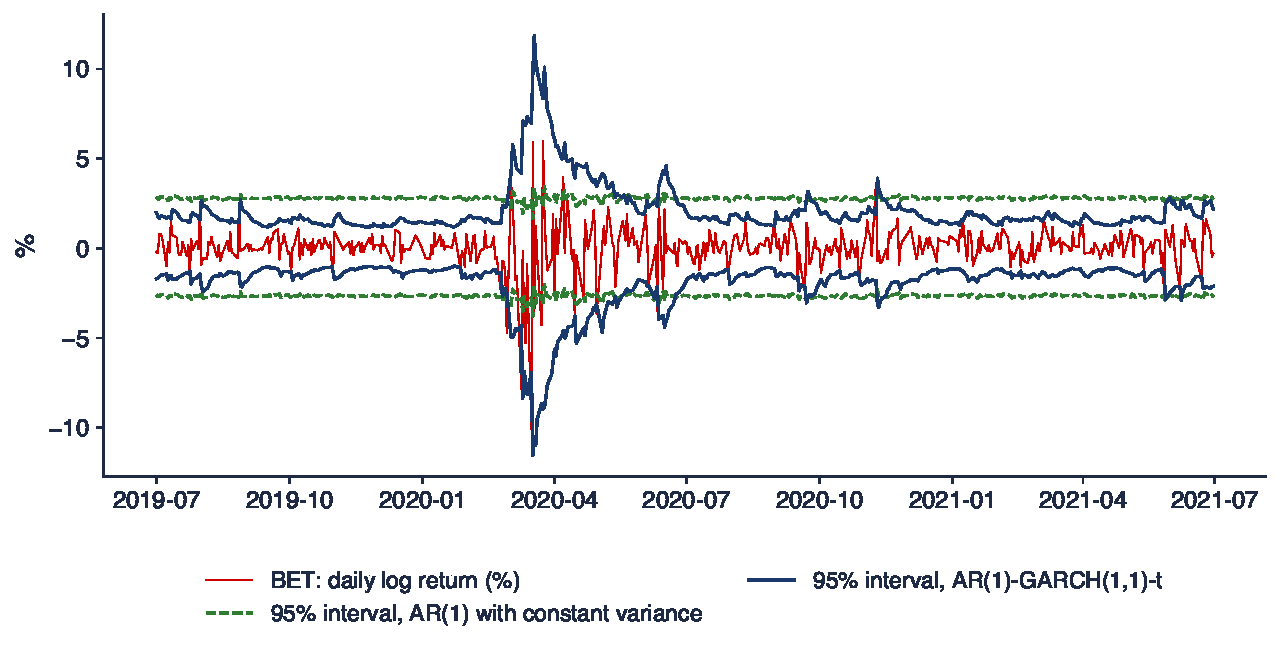
\includegraphics[width=0.97\textwidth,height=0.52\textheight,keepaspectratio]{tsa_ch5_bands.pdf}
\end{center}
\vspace{-0.25cm}
\begin{itemize}
    \item BET, one-day-ahead 95\% intervals: AR(1) with constant variance (width 5.4 points every day) and AR(1)-GARCH(1,1)-t (width from 2.2 to 22.5 points in this window)
\end{itemize}
\quantlet{TSA\_ch5\_arma\_garch}{\qlurl{TSA_ch5_arma_garch}}
\end{frame}

\begin{frame}{Interpreting the two intervals}
\itemsize{\small}
\begin{itemize}
    \item Over the whole sample both miss about 5\% of the days: 5.0\% and 5.2\%
    \begin{itemize}
        \item the constant interval is right on average, but wrong almost every day
    \end{itemize}
    \item In 2017 (calm): the constant interval misses 0.4\% of the days, the GARCH interval 2.0\%
    \begin{itemize}
        \item in March--April 2020: 33.3\% against 9.5\%: the misses of the constant interval cluster in crises
    \end{itemize}
    \item \tsachlink{https://danpele.github.io/Time-Series-Analysis/EN/Courses/chapter2_arma_models.pdf}{Chapter 2} gave intervals whose width depends only on the horizon; with GARCH it also depends on the current state
\end{itemize}
\end{frame}

\begin{frame}{Recap: four markets and ARMA-GARCH}
\itemsize{\small}
\begin{itemize}
    \item $\alpha + \beta$ close to 1 everywhere; EUR/RON and Bitcoin are IGARCH
    \item The long-run volatility is imprecise when $\alpha + \beta$ is near 1
    \item ARMA-GARCH: the mean of \tsachlink{https://danpele.github.io/Time-Series-Analysis/EN/Courses/chapter2_arma_models.pdf}{Chapter 2} with GARCH errors; joint MLE; intervals that follow the volatility
\end{itemize}
\end{frame}


%=============================================================================
\section{Asymmetry and the leverage effect}
%=============================================================================

\begin{frame}{The leverage effect and the news impact curve}
\itemsize{\small}
\begin{itemize}
    \item \textbf{Leverage effect}: falls in stock prices raise volatility more than rises of the same size \refChristie
    \begin{itemize}
        \item a lower share price raises the debt-to-equity ratio, so the equity becomes riskier; news of higher risk also lowers prices at once
    \end{itemize}
    \item GARCH(1,1) cannot see it: $\sigma_t^2$ depends on $\varepsilon_{t-1}^2$, not on the sign of $\varepsilon_{t-1}$
    \begin{itemize}
        \item the QQ plot and the skewed t ($\hat\lambda < 0$) already pointed to the left tail
    \end{itemize}
    \item \textbf{NIC} (news impact curve) \refEN: $\sigma_t^2$ as a function of $\varepsilon_{t-1}$, with $\sigma_{t-1}^2$ fixed at the unconditional variance; for GARCH, a symmetric parabola
\end{itemize}
\end{frame}

\begin{frame}{GJR-GARCH and EGARCH}
\itemsize{\small}
\begin{itemize}
    \item \textbf{GJR-GARCH} \refGJR: $\sigma_t^2 = \omega + (\alpha + \gamma\,I_{t-1})\,\varepsilon_{t-1}^2 + \beta\sigma_{t-1}^2$, with $I_{t-1} = 1$ if $\varepsilon_{t-1} < 0$, else 0
    \begin{itemize}
        \item good news: slope $\alpha$; bad news: $\alpha + \gamma$; leverage effect: $\gamma > 0$; in \texttt{arch}: \texttt{o=1}
        \item persistence $\alpha + \beta + \gamma/2$ for symmetric $z_t$ (half of the shocks are negative)
    \end{itemize}
    \item \textbf{EGARCH} (exponential GARCH) \refNelson: $\ln\sigma_t^2 = \omega + \alpha\big(|z_{t-1}| - E|z_{t-1}|\big) + \gamma z_{t-1} + \beta\ln\sigma_{t-1}^2$
    \begin{itemize}
        \item the logarithm keeps $\sigma_t^2 > 0$ without sign restrictions; leverage effect: $\gamma < 0$; persistence: $\beta$
    \end{itemize}
    \item Both have one parameter more than GARCH(1,1); test $\gamma = 0$ with its $t$ statistic or with an LR test, $\chi^2(1)$
\end{itemize}
\end{frame}

\begin{frame}{News impact curves: S\&P 500 and Bitcoin}
\itemsize{\footnotesize}
\begin{center}
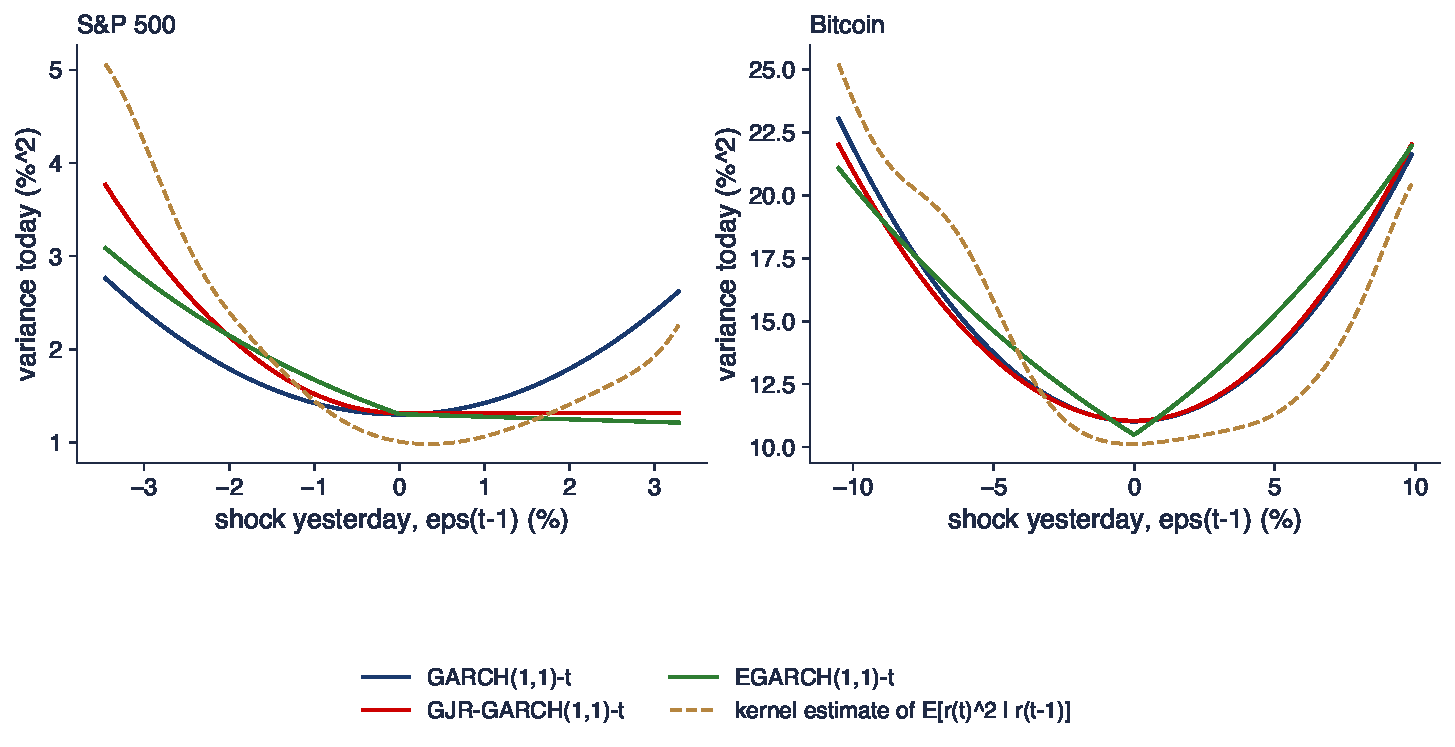
\includegraphics[width=0.97\textwidth,height=0.54\textheight,keepaspectratio]{tsa_ch5_nic.pdf}
\end{center}
\vspace{-0.25cm}
\begin{itemize}
    \item Model curves: $\sigma_t^2$ against $\varepsilon_{t-1}$, with $\sigma_{t-1}^2$ at the sample variance; dashed: a kernel (Nadaraya--Watson) estimate of $E[r_t^2 \mid r_{t-1}]$, without a model
    \item S\&P 500, GJR: after a fall of 2\%, tomorrow's variance is 1.62 times the variance after a rise of 2\%; Bitcoin: ratio 1.00, a symmetric curve
\end{itemize}
\quantlet{TSA\_ch5\_asymmetry}{\qlurl{TSA_ch5_asymmetry}}
\end{frame}

\begin{frame}{Asymmetry in four markets}
\itemsize{\footnotesize}
\begin{center}
\scriptsize
\begin{tabular}{lrrrrrrrr}
\toprule
& GJR $\alpha$ & GJR $\gamma$ & $t(\gamma)$ & LR & p & $\Delta$BIC & EGARCH $\gamma$ & $t(\gamma)$ \\
\midrule
S\&P 500 & $0.000$ & $0.205$ & $10.0$ & $235.7$ & $<$\,0.001 & ${-226.8}$ & ${-0.165}$ & ${-15.2}$ \\
BET & $0.172$ & $0.043$ & $2.1$ & $4.9$ & 0.026 & ${3.9}$ & ${-0.028}$ & ${-2.6}$ \\
EUR/RON & $0.103$ & $0.039$ & $3.0$ & $9.3$ & 0.002 & ${-0.7}$ & ${-0.040}$ & ${-2.5}$ \\
Bitcoin & $0.113$ & $-0.013$ & $-0.7$ & $0.7$ & 0.416 & ${7.7}$ & ${0.015}$ & ${1.2}$ \\
\bottomrule
\end{tabular}
\end{center}
\begin{itemize}
    \item Student-t innovations; robust $t$ statistics; LR $= 2(\ell_{GJR} - \ell_{GARCH}) \sim \chi^2(1)$; $\Delta$BIC: GJR minus GARCH (negative: GJR preferred)
    \item S\&P 500: GJR $\hat\alpha = 0.000$: only bad news raises volatility; a very strong leverage effect
    \item BET: weak, significant by LR, but BIC prefers GARCH; Bitcoin: none; EUR/RON: $r_t > 0$ means a weaker leu, so the ``bad news'' of GJR are days when the leu strengthens
    \item Interpretation: leverage is a property of mature equity markets, not of every financial series
\end{itemize}\quantlet{TSA\_ch5\_asymmetry}{\qlurl{TSA_ch5_asymmetry}}
\end{frame}

\begin{frame}{Recap: asymmetry}
\itemsize{\small}
\begin{itemize}
    \item GJR: an extra slope $\gamma$ for negative shocks; EGARCH: a sign term $\gamma z_{t-1}$ in $\ln\sigma_t^2$
    \item The news impact curve shows the asymmetry at a glance
    \item Strong in the S\&P 500, weak in the BET, absent in Bitcoin
\end{itemize}
\end{frame}


%=============================================================================
\section{Diagnostics and model choice}
%=============================================================================

\begin{frame}{Checking a fitted model}
\itemsize{\small}
\begin{itemize}
    \item If the model is right, the \textbf{standardised residuals} $\hat z_t = (r_t - \hat\mu_t)/\hat\sigma_t$ are close to i.i.d.\ with mean 0 and variance 1
    \begin{itemize}
        \item Ljung--Box $Q(10)$ on $\hat z_t$: no autocorrelation left in the mean (the check of \tsachlink{https://danpele.github.io/Time-Series-Analysis/EN/Courses/chapter2_arma_models.pdf}{Chapter 2})
        \item Ljung--Box $Q(10)$ on $\hat z_t^2$ and ARCH-LM on $\hat z_t$: no ARCH effects left
        \item QQ plot of $\hat z_t$: is the assumed distribution right?
    \end{itemize}
    \item \textbf{Sign-bias test} \refEN: regress $\hat z_t^2$ on $I_{t-1}$, $I_{t-1}\hat\varepsilon_{t-1}$ and $(1 - I_{t-1})\hat\varepsilon_{t-1}$
    \begin{itemize}
        \item joint test $T R^2 \sim \chi^2(3)$: a rejection means that the sign of past shocks still predicts the variance
    \end{itemize}
    \item A passed diagnostic does not prove the model right; a failed one shows where it is wrong
\end{itemize}
\end{frame}

\begin{frame}{What GARCH removes}
\itemsize{\footnotesize}
\begin{center}
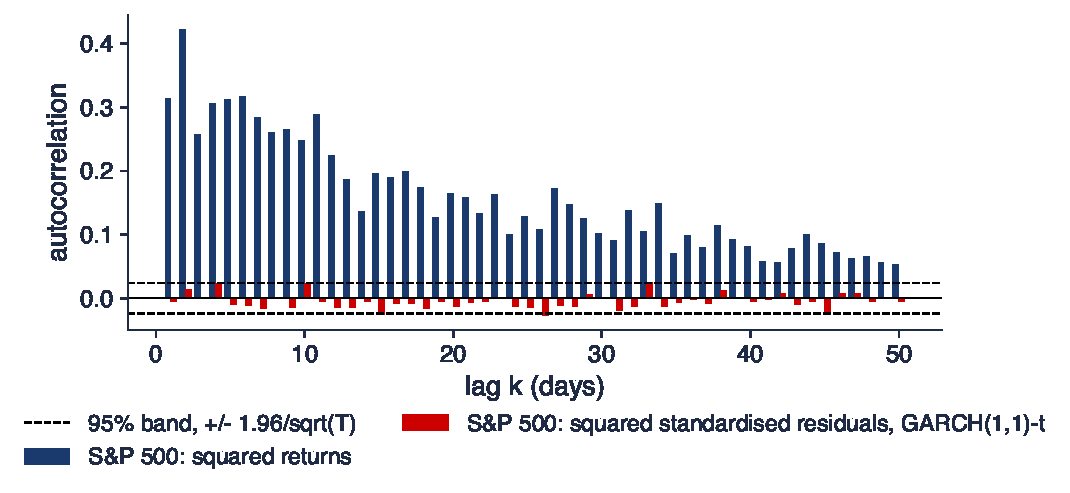
\includegraphics[width=0.97\textwidth,height=0.48\textheight,keepaspectratio]{tsa_ch5_acf_diag.pdf}
\end{center}
\vspace{-0.25cm}
\begin{itemize}
    \item S\&P 500: ACF of $r_t^2$: $0.31$ at lag 1, still $0.053$ at lag 50; ACF of $\hat z_t^2$ (GARCH(1,1)-t): $-0.005$ at lag 1, at most $0.028$ in absolute value; band $\pm0.024$
    \item Interpretation: four parameters absorb almost all the volatility clustering of 27 years of daily data
\end{itemize}
\quantlet{TSA\_ch5\_diagnostics}{\qlurl{TSA_ch5_diagnostics}}
\end{frame}

\begin{frame}{Diagnostics on real data}
\itemsize{\footnotesize}
\begin{center}
\scriptsize
\begin{tabular}{lrrr}
\toprule
S\&P 500 & $Q(10)$ (p) & $Q(10)$ of squares (p) & ARCH-LM(5) (p) \\
\midrule
returns $r_t$ & $96.3$ ($<$\,0.001) & $6133$ ($<$\,0.001) & $1684$ ($<$\,0.001) \\
$\hat z_t$, GARCH-N & $21.2$ (0.020) & $16.4$ (0.089) & $7.0$ (0.222) \\
$\hat z_t$, GARCH-t & $21.9$ (0.016) & $13.6$ (0.192) & $4.8$ (0.438) \\
\bottomrule
\end{tabular}
\end{center}
\begin{itemize}
    \item GARCH removes the ARCH effects ($Q(10)$ of squares: from $6133$ to $13.6$); a little autocorrelation remains in the mean (constant mean; an AR(1) helps, Section 6)
    \item Sign bias for the GARCH-t of the S\&P 500: $\chi^2(3) = 40.7$ (p $<$\,0.001): the asymmetry of Section 7 is missing
    \item $Q(10)$ of $\hat z_t^2$, GARCH-t: BET 8.3 (p = 0.596), Bitcoin 4.7 (p = 0.910), EUR/RON 0.004: suspiciously small (next slide)
\end{itemize}\quantlet{TSA\_ch5\_diagnostics}{\qlurl{TSA_ch5_diagnostics}}
\end{frame}

\begin{frame}{Case study: the EUR/RON on 6 May 2025}
\itemsize{\footnotesize}
\begin{columns}[T]
\begin{column}{0.62\textwidth}
\begin{itemize}
    \item In April 2025 the reference rate moved by 0.0038\% a day on average: the BNR held the leu almost fixed
    \begin{itemize}
        \item the IGARCH volatility fell to $\hat\sigma_t = 0.0078\%$; then the rate rose by 1.20\% (two days after the first round of the presidential election) and by 1.21\% the next day
    \end{itemize}
    \item Standardised residual: $\hat z_t = 154$, a ``154-sigma'' day; the next largest is 13.2
    \begin{itemize}
        \item $Q(10)$ of $\hat z_t^2$: 0.004 with this day, 19.2 (p = 0.038) without it: one value hides the remaining ARCH effects
    \end{itemize}
    \item Lesson: a managed rate is not a free market; GARCH cannot foresee a policy decision; always plot $\hat z_t$ before trusting a test
\end{itemize}
\end{column}
\begin{column}{0.34\textwidth}
\centering
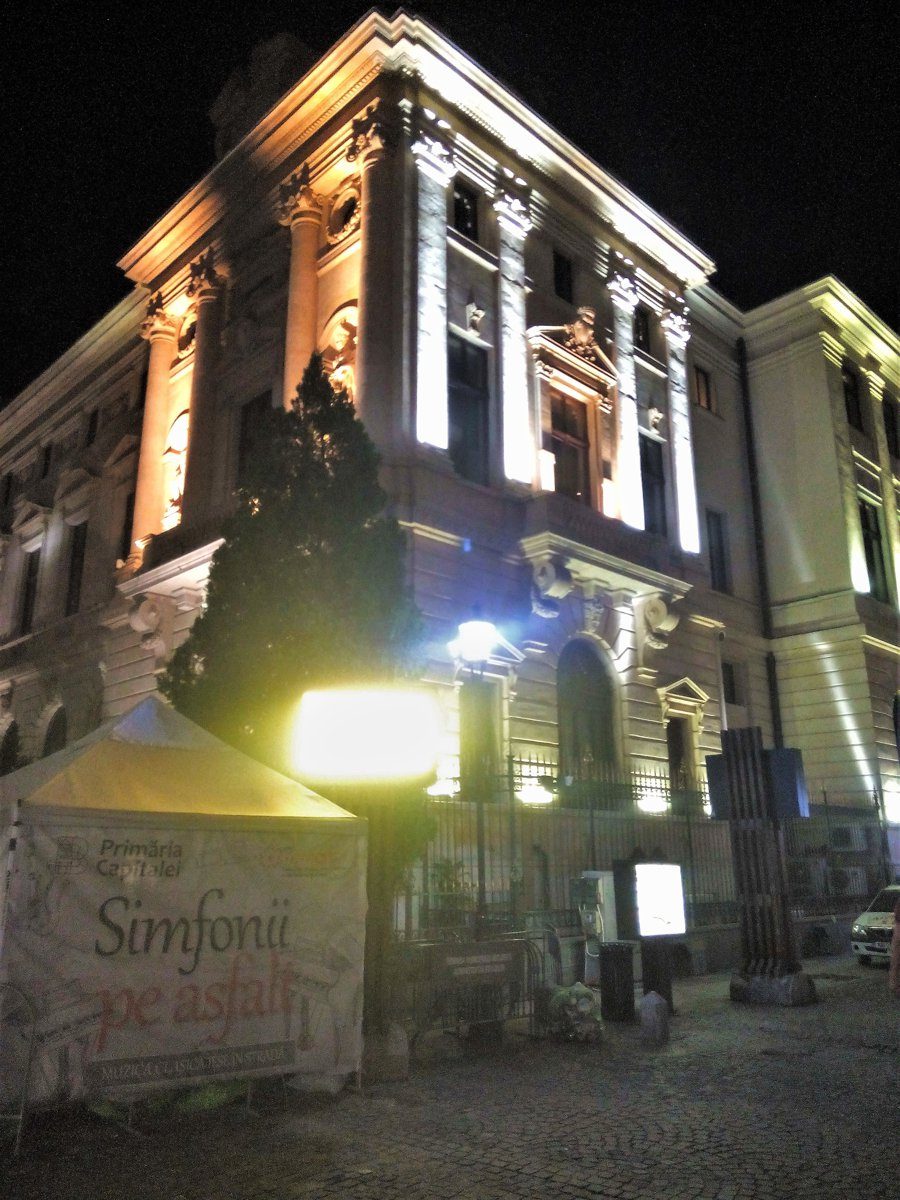
\includegraphics[height=0.28\textheight]{ch1_bnr_2018.jpg}\\[1mm]
\imgcap{The National Bank of Romania, Bucharest}
\imgcredit{https://commons.wikimedia.org/wiki/File:National_Bank_of_Romania_(old_building),_Bucharest_by_nickispeaki_01.jpg}{Photo: Nickispeaki (2018); CC BY-SA 4.0; Wikimedia Commons}
\end{column}
\end{columns}
\vspace{1mm}
\quantlet{TSA\_ch5\_diagnostics}{\qlurl{TSA_ch5_diagnostics}}
\end{frame}

\begin{frame}{Nine models for the S\&P 500}
\itemsize{\footnotesize}
\begin{itemize}
    \item AIC $= -2\ell + 2k$ \refAkaike; BIC $= -2\ell + k\ln T$ \refSchwarz; $k$ parameters; compare models fitted on the same data
\end{itemize}\begin{center}
\scriptsize
\begin{tabular}{lrrrrrr}
\toprule
& \multicolumn{2}{c}{Normal} & \multicolumn{2}{c}{Student-t} & \multicolumn{2}{c}{skewed t} \\ & log-lik. & $\Delta$BIC & log-lik. & $\Delta$BIC & log-lik. & $\Delta$BIC \\
\midrule
GARCH(1,1) & -9218.0 & 648.9 & -9062.5 & 346.7 & -9038.4 & 307.4 \\
GJR-GARCH(1,1) & -9086.5 & 394.7 & -8944.6 & 119.9 & -8905.1 & 49.6 \\
EGARCH(1,1) & -9075.6 & 372.9 & -8922.1 & 74.8 & -8880.3 & 0.0 \\
\bottomrule
\end{tabular}
\end{center}
\begin{itemize}
    \item $\Delta$BIC: the difference from the best model, EGARCH-skewed t
    \item From the Normal GARCH: asymmetry alone (Normal EGARCH) lowers BIC by 276, heavy tails alone (GARCH-skewed t) by 341, both by 649
    \item Interpretation: with 6\,714 observations even small gains are ``significant''; the out-of-sample comparison of Section 9 is the real test
\end{itemize}\quantlet{TSA\_ch5\_diagnostics}{\qlurl{TSA_ch5_diagnostics}}
\end{frame}

\begin{frame}{Recap: diagnostics and model choice}
\itemsize{\small}
\begin{itemize}
    \item Standardised residuals: no autocorrelation in $\hat z_t$ and $\hat z_t^2$, the right distribution, no sign bias
    \item One extreme $\hat z_t$ can hide everything: plot before testing
    \item AIC/BIC on the same data; in-sample fit is not forecasting ability
\end{itemize}
\end{frame}


%=============================================================================
\section{Variance forecasts and their evaluation}
%=============================================================================

\begin{frame}{Multi-step forecasts}
\itemsize{\small}
\begin{itemize}
    \item One step: $\sigma_{t+1}^2 = \omega + \alpha\varepsilon_t^2 + \beta\sigma_t^2$ is known at the end of day $t$
    \begin{itemize}
        \item two steps: $E_t[\sigma_{t+2}^2] = \omega + \alpha E_t[\varepsilon_{t+1}^2] + \beta\sigma_{t+1}^2 = \omega + (\alpha + \beta)\sigma_{t+1}^2$, since $E_t[\varepsilon_{t+1}^2] = \sigma_{t+1}^2$
    \end{itemize}
    \item By induction: $E_t[\sigma_{t+h}^2] = \bar\sigma^2 + (\alpha + \beta)^{h-1}(\sigma_{t+1}^2 - \bar\sigma^2)$
    \begin{itemize}
        \item the forecast converges to the long-run variance, like an AR(1) forecast converges to its mean (\tsachlink{https://danpele.github.io/Time-Series-Analysis/EN/Courses/chapter2_arma_models.pdf}{Chapter 2})
    \end{itemize}
    \item Variance of the $H$-day return: the sum of the daily forecasts (the returns are uncorrelated)
    \begin{itemize}
        \item $\mathrm{Var}_t(r_{t+1} + \dots + r_{t+H}) = \sum_{h=1}^{H} E_t[\sigma_{t+h}^2]$, not $H\sigma_{t+1}^2$
        \item the square-root-of-time rule $\sigma_{t+1}\sqrt{H}$ is too high in a crisis and too low in a calm period
    \end{itemize}
\end{itemize}
\end{frame}

\begin{frame}{Worked example: the S\&P 500 on 18 September 2026}
\itemsize{\small}
\begin{itemize}
    \item GARCH(1,1)-t: $\alpha + \beta = 0.9947$, $\bar\sigma^2 = 2.972$; forecast for the next day $\sigma_{t+1}^2 = 0.509$ (below the long-run level)
    \item Step by step
    \begin{itemize}
        \item day 10: $2.972 + 0.9947^{9}(0.509 - 2.972) = 2.972 + 0.953 \times (0.509 - 2.972) = 0.624$
        \item 10-day variance: the sum of the ten daily forecasts $= 5.67$, so the 10-day volatility is $2.38\%$
        \item square-root-of-time rule: $\sqrt{10 \times 0.509} = 2.26\%$: too low, because volatility is expected to rise towards its long-run level
    \end{itemize}
\end{itemize}
\end{frame}

\begin{frame}{The term structure of volatility}
\itemsize{\footnotesize}
\begin{center}
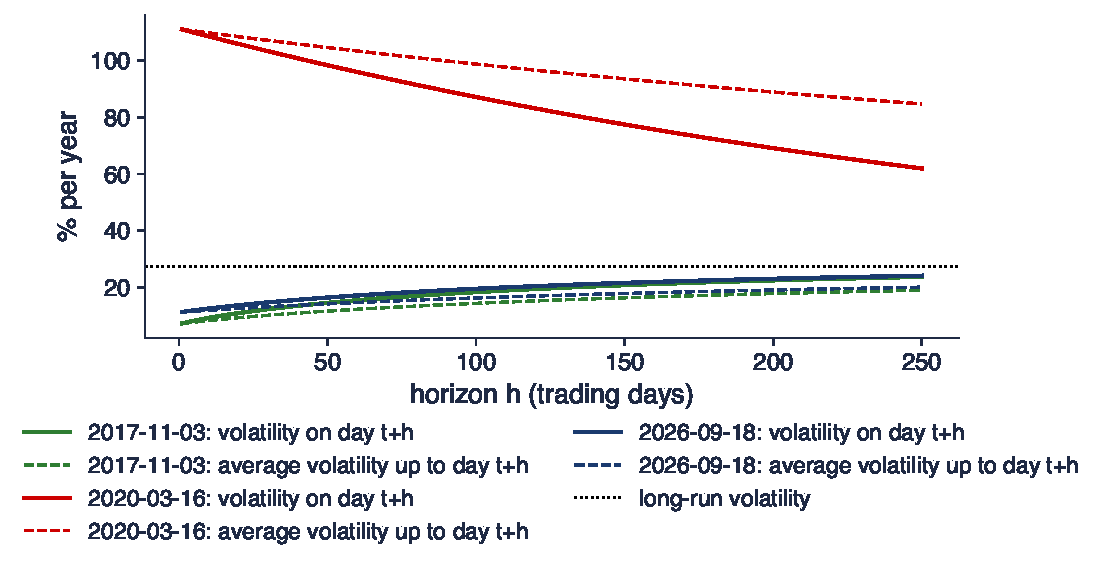
\includegraphics[width=0.97\textwidth,height=0.46\textheight,keepaspectratio]{tsa_ch5_term_structure.pdf}
\end{center}
\vspace{-0.25cm}
\begin{itemize}
    \item S\&P 500, GARCH(1,1)-t on all data; forecasts made on a calm day (3 November 2017), at the COVID-19 peak (16 March 2020) and on 18 September 2026
    \item Calm day: 7.3\% tomorrow, 19.0\% on average over a year; COVID-19 peak: 111.0\% tomorrow, still 84.7\% on average over a year
    \item Interpretation: all curves move towards the long-run level (27.3\%) at the same slow speed; the slope tells whether we are in a calm period or in a storm
\end{itemize}
\quantlet{TSA\_ch5\_forecasts}{\qlurl{TSA_ch5_forecasts}}
\end{frame}

\begin{frame}{How to evaluate a volatility forecast}
\itemsize{\small}
\begin{itemize}
    \item The true $\sigma_t^2$ is never observed: we compare the forecast $h_t$ with a noisy \textbf{proxy}, here $r_t^2$
    \begin{itemize}
        \item $E_{t-1}[r_t^2] = \sigma_t^2$ (with $\mu \approx 0$), but $r_t^2$ is very noisy: a low $R^2$ even for a perfect forecast \refAB
    \end{itemize}
    \item \textbf{QLIKE} loss \refPatton: $L(r_t^2, h_t) = \dfrac{r_t^2}{h_t} + \ln h_t$ (up to a constant); the smaller the mean, the better
    \begin{itemize}
        \item it ranks forecasts correctly even with a noisy proxy; it is minus the Normal log-likelihood; it punishes forecasts that are too low
    \end{itemize}
    \item \textbf{Out of sample} (\tsachlink{https://danpele.github.io/Time-Series-Analysis/EN/Courses/chapter0_introduction.pdf}{Chapter 0}): from 2015, each forecast uses only data up to the day before; the models are re-estimated every 250 days
    \begin{itemize}
        \item \textbf{DM} (Diebold--Mariano) test \refDM: is the mean loss difference zero? $t$ statistic with HAC (heteroskedasticity and autocorrelation consistent) standard errors
    \end{itemize}
\end{itemize}
\end{frame}

\begin{frame}{GARCH against EWMA, out of sample}
\itemsize{\footnotesize}
\begin{center}
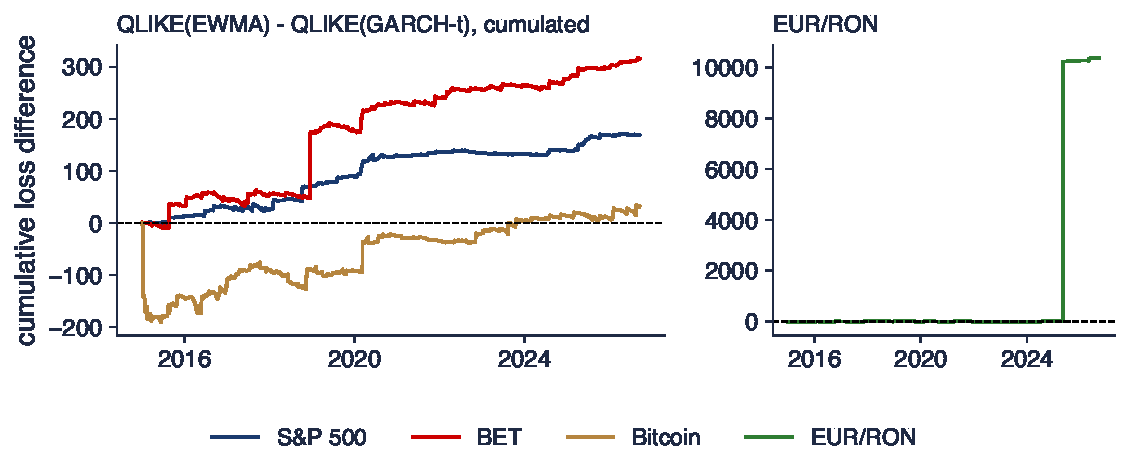
\includegraphics[width=0.97\textwidth,height=0.50\textheight,keepaspectratio]{tsa_ch5_forecast_eval.pdf}
\end{center}
\vspace{-0.25cm}
\begin{itemize}
    \item One-day-ahead variance forecasts from 2015 to 18 September 2026: GARCH(1,1)-t (re-estimated every 250 days) against EWMA with $\lambda = 0.94$; a rising curve means that GARCH-t has the smaller QLIKE
\end{itemize}
\quantlet{TSA\_ch5\_forecasts}{\qlurl{TSA_ch5_forecasts}}
\end{frame}

\begin{frame}{Interpreting the forecast comparison}
\itemsize{\footnotesize}
\begin{center}
\scriptsize
\begin{tabular}{lrrrrr}
\toprule
2015--2026 & days & QLIKE GARCH-t & QLIKE GJR-t & QLIKE EWMA & DM $t$, GARCH-t against EWMA (p) \\
\midrule
S\&P 500 & 2\,944 & $0.761$ & $0.733$ & $0.819$ & ${-3.69}$ ($<$\,0.001) \\
BET & 2\,926 & $0.680$ & $0.674$ & $0.788$ & ${-2.22}$ (0.027) \\
EUR/RON & 2\,939 & $2.456$ & $3.276$ & $5.982$ & ${-1.02}$ (0.310) \\
Bitcoin & 4\,279 & $3.383$ & $3.401$ & $3.390$ & ${-0.20}$ (0.845) \\
\bottomrule
\end{tabular}
\end{center}
\begin{itemize}
    \item S\&P 500 and BET: GARCH-t beats EWMA ($t < -1.96$); GJR-t has the smallest QLIKE (the leverage effect pays off out of sample)
    \item Bitcoin: no difference ($t = -0.20$): its GARCH is an IGARCH, which is almost an EWMA
    \item EUR/RON: a much smaller mean QLIKE for GARCH, yet $t = -1.02$: 98\% of the total difference comes from one day, 6 May 2025, when EWMA forecast a near-zero variance
    \item Interpretation: QLIKE punishes forecasts that are too low; the DM test protects us from conclusions built on a single day
\end{itemize}\quantlet{TSA\_ch5\_forecasts}{\qlurl{TSA_ch5_forecasts}}
\end{frame}

\begin{frame}{Case study: Hansen and Lunde (2005)}
\itemsize{\small}
\begin{itemize}
    \item \textbf{Question}: does anything beat a GARCH(1,1)? \refHL
    \begin{itemize}
        \item 330 ARCH-type models (asymmetric, long memory, different innovations), compared out of sample on the Deutsche Mark/US dollar exchange rate and on the returns of one US stock
        \item the proxy: realised variance from intraday returns, more precise than $r_t^2$
    \end{itemize}
    \item \textbf{Finding}: for the exchange rate, no model beat GARCH(1,1) significantly; for the stock, models with a leverage effect did better
    \begin{itemize}
        \item the same pattern as our table: asymmetry matters for equities, not for currencies or Bitcoin
    \end{itemize}
    \item \textbf{Legacy}: GARCH(1,1) is the benchmark every new volatility model, including machine learning (Chapter 9), must beat out of sample
\end{itemize}
\end{frame}

\begin{frame}{Recap: variance forecasts}
\itemsize{\small}
\begin{itemize}
    \item $E_t[\sigma_{t+h}^2] = \bar\sigma^2 + (\alpha + \beta)^{h-1}(\sigma_{t+1}^2 - \bar\sigma^2)$; $H$-day variance = sum of the daily forecasts
    \item Compare forecasts out of sample with QLIKE and the Diebold--Mariano test
    \item GARCH beats EWMA where volatility mean-reverts
\end{itemize}
\end{frame}


%=============================================================================
\section{An application: VaR 1\% from a GARCH model}
%=============================================================================

\begin{frame}{Conditional VaR}
\itemsize{\small}
\begin{itemize}
    \item \textbf{VaR} (value at risk) at level $\alpha$: the loss exceeded with probability $\alpha$, $\mathrm{VaR}_\alpha = -q_\alpha(r_{t+1})$, with $q_\alpha$ the $\alpha$-quantile
    \begin{itemize}
        \item here $\alpha = 1\%$: VaR 1\%, a loss exceeded on one day in a hundred
    \end{itemize}
    \item With $r_{t+1} = \mu + \sigma_{t+1}z_{t+1}$: $\mathrm{VaR}_{t+1} = -(\mu + \sigma_{t+1}\,q_\alpha(z))$
    \begin{itemize}
        \item Normal: $q_{0.01} = -2.326$; standardised t: $q_{0.01} = t_\nu^{-1}(0.01)\sqrt{(\nu - 2)/\nu}$
        \item the VaR moves every day with $\sigma_{t+1}$: high in storms, low in calm periods
    \end{itemize}
    \item \textbf{Worked example}: S\&P 500 on 18 September 2026, GARCH(1,1)-t: $\hat\mu = 0.079$, $\sigma_{t+1} = 0.714$, $\hat\nu = 6.26$
    \begin{itemize}
        \item $q = -3.100 \times 0.825 = -2.557$; VaR 1\% $= -(0.079 + 0.714 \times (-2.557)) = 1.75\%$
        \item with Normal $z_t$: $1.58\%$; over 10 days (sum of the variances, $\mu$ ignored): $2.557 \times \sqrt{5.67} = 6.09\%$
    \end{itemize}
\end{itemize}
\end{frame}

\begin{frame}{VaR 1\% through the COVID-19 crash}
\itemsize{\footnotesize}
\begin{center}
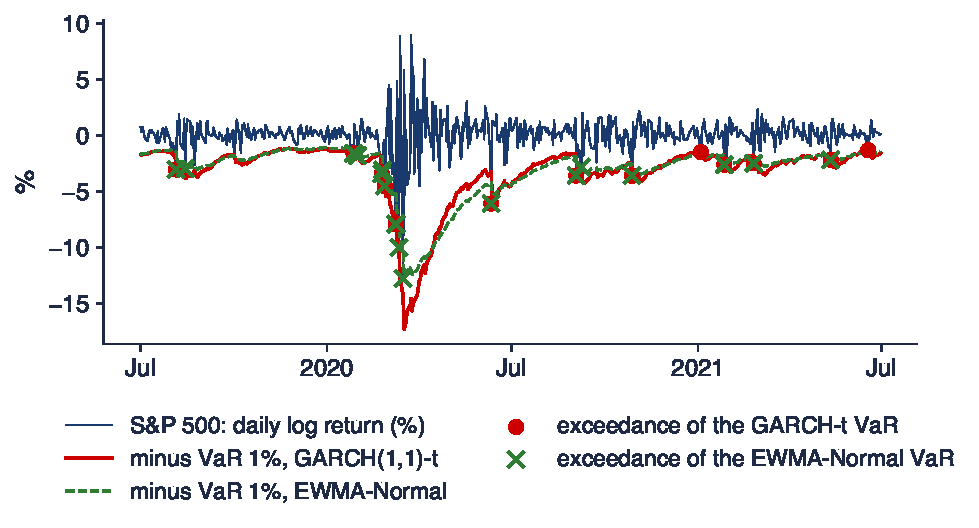
\includegraphics[width=0.97\textwidth,height=0.48\textheight,keepaspectratio]{tsa_ch5_var.pdf}
\end{center}
\vspace{-0.25cm}
\begin{itemize}
    \item S\&P 500, July 2019 -- June 2021 (505 days): one-day VaR 1\% from GARCH(1,1)-t (re-estimated every 250 days) and from EWMA with Normal $z_t$
    \item Exceedances (return below $-$VaR): GARCH-t 13, EWMA-Normal 17, about 5 expected; both models react, but only after the first large falls of March 2020
\end{itemize}
\quantlet{TSA\_ch5\_forecasts}{\qlurl{TSA_ch5_forecasts}}
\end{frame}

\begin{frame}{Exceedances 2015--2026}
\itemsize{\footnotesize}
\begin{center}
\footnotesize
\begin{tabular}{lrrrr}
\toprule
VaR 1\% & days & expected & GARCH-t & EWMA-Normal \\
\midrule
S\&P 500 & 2\,944 & 29 & 49 (1.66\%) & 65 (2.21\%) \\
BET & 2\,926 & 29 & 34 (1.16\%) & 67 (2.29\%) \\
EUR/RON & 2\,939 & 29 & 35 (1.19\%) & 63 (2.14\%) \\
Bitcoin & 4\,279 & 43 & 64 (1.50\%) & 93 (2.17\%) \\
\bottomrule
\end{tabular}
\end{center}
\begin{itemize}
    \item A correct VaR 1\% is exceeded on 1\% of the days, and the exceedances do not cluster
    \item EWMA-Normal: 2.1--2.3\% everywhere: the Normal quantile is too small for heavy tails
    \item GARCH-t: 1.2--1.7\%: much closer to 1\%; the highest for the S\&P 500, where the leverage effect is missing
    \item Are the differences significant? The test of \refKupiec\ compares the number of exceedances with a binomial distribution
\end{itemize}\quantlet{TSA\_ch5\_forecasts}{\qlurl{TSA_ch5_forecasts}}
\end{frame}

\begin{frame}{Recap: VaR 1\% from a GARCH model}
\itemsize{\small}
\begin{itemize}
    \item $\mathrm{VaR}_{t+1} = -(\mu + \sigma_{t+1}q_\alpha(z))$: a dynamic volatility and the right quantile
    \item Normal quantiles underestimate the risk; Student-t is much closer to 1\%
    \item Several series at once (covariances of returns): multivariate GARCH, Chapter 14 (self-study)
\end{itemize}
\end{frame}


%=============================================================================
\section{Possible contribution of AI}
%=============================================================================

\begin{frame}{Possible contribution of AI}
\itemsize{\small}
\begin{itemize}
    \item \textbf{Code}: a first draft of a script that runs ARCH-LM, fits GARCH, GJR and EGARCH with \texttt{arch} on many series and tabulates the results
    \item \textbf{Explanation}: a second explanation of the ARMA(1,1) form of GARCH, or of an \texttt{arch} output table
    \item \textbf{Exploration}: volatility of all BVB stocks, or of the leu against several currencies
    \item Example prompt
    \begin{itemize}
        \item \aiprompt{Write Python code that loads daily BET closes, computes log returns in percent, runs the ARCH-LM test with 5 lags, fits AR(1)-GARCH(1,1) with Student-t innovations using the arch package, and plots the annualised conditional volatility.}
    \end{itemize}
\end{itemize}
\end{frame}

\begin{frame}{Checks you must run}
\itemsize{\small}
\begin{itemize}
    \item Units: returns in \%, not decimals; rescale a series with a very small variance (EUR/RON) and convert $\omega$ back
    \item The persistence: $\alpha + \beta$ for GARCH, $\alpha + \beta + \gamma/2$ for GJR, $\beta$ for EGARCH
    \item Boundary estimates ($\alpha + \beta = 1$): no half-life and no long-run volatility; do not report infinite numbers
    \item Calendars: Bitcoin trades 7 days a week, the BET five; annualise each series with its own frequency
    \item Out-of-sample forecasts use only past data; the VaR level is written as VaR 1\%
    \item Every cited reference: it must exist; check the DOI
\end{itemize}
\end{frame}


%=============================================================================
\section{Summary}
%=============================================================================

\begin{frame}{Key takeaways}
\itemsize{\small}
\begin{itemize}
    \item Returns: an almost unpredictable mean and a predictable variance, $r_t = \mu_t + \sigma_t z_t$; test with the ACF of $r_t^2$ and ARCH-LM
    \item GARCH(1,1) is an ARMA(1,1) for $\varepsilon_t^2$; $\alpha + \beta$ close to 1; IGARCH and EWMA when $\alpha + \beta = 1$
    \item Estimate by maximum likelihood with \texttt{arch}, report robust SE; Student-t innovations for the tails
    \item ARMA-GARCH: the mean of \tsachlink{https://danpele.github.io/Time-Series-Analysis/EN/Courses/chapter2_arma_models.pdf}{Chapter 2} and the variance of this chapter estimated together
    \item Equity indices need asymmetry (GJR, EGARCH); check $\hat z_t$ and $\hat z_t^2$ after every fit
    \item Forecasts revert to the long-run level; compare them out of sample with QLIKE and DM; VaR 1\% $= -(\mu + \sigma_{t+1}q_{0.01}(z))$
\end{itemize}
\end{frame}

\begin{frame}{Key formulas}
\itemsize{\small}
{\renewcommand{\arraystretch}{1.4}\begin{center}
\scriptsize
\begin{tabular}{ll}
\toprule
\textbf{Quantity} & \textbf{Formula} \\
\midrule
ARCH-LM & $\hat\varepsilon_t^2 = b_0 + \sum_{i=1}^{q}b_i\hat\varepsilon_{t-i}^2 + u_t$, \quad $\mathrm{LM} = nR^2 \sim \chi^2(q)$ \\
ARCH($q$) & $\sigma_t^2 = \omega + \sum_{i=1}^{q}\alpha_i\varepsilon_{t-i}^2$, \quad $\bar\sigma^2 = \omega/(1 - \sum\alpha_i)$ \\
GARCH(1,1) & $\sigma_t^2 = \omega + \alpha\varepsilon_{t-1}^2 + \beta\sigma_{t-1}^2$, \quad $\bar\sigma^2 = \omega/(1 - \alpha - \beta)$, \quad $h_{1/2} = \ln 0.5/\ln(\alpha + \beta)$ \\
EWMA & $\sigma_t^2 = \lambda\sigma_{t-1}^2 + (1 - \lambda)r_{t-1}^2$ \\
GJR, EGARCH & $\sigma_t^2 = \omega + (\alpha + \gamma I_{t-1})\varepsilon_{t-1}^2 + \beta\sigma_{t-1}^2$; \quad $\ln\sigma_t^2 = \omega + \alpha(|z_{t-1}| - E|z_{t-1}|) + \gamma z_{t-1} + \beta\ln\sigma_{t-1}^2$ \\
Log-likelihood & $\ell = -\frac12\sum_t[\ln 2\pi + \ln\sigma_t^2 + (r_t - \mu_t)^2/\sigma_t^2]$ \\
Forecast & $E_t[\sigma_{t+h}^2] = \bar\sigma^2 + (\alpha + \beta)^{h-1}(\sigma_{t+1}^2 - \bar\sigma^2)$ \\
QLIKE, VaR 1\% & $L = r_t^2/h_t + \ln h_t$; \quad $\mathrm{VaR}_{t+1} = -(\mu + \sigma_{t+1}\,q_{0.01}(z))$ \\
\bottomrule
\end{tabular}
\end{center}
}
\end{frame}

\begin{frame}{Self-assessment}
\itemsize{\small}
\begin{itemize}
    \item \textbf{Question}: $\omega = 0.05$, $\alpha = 0.05$, $\beta = 0.90$. What are the long-run variance and the half-life?
    \begin{itemize}
        \item \textbf{Answer}: $0.05/0.05 = 1$; $\ln 0.5/\ln 0.95 = 13.5$ days
    \end{itemize}
    \item \textbf{Question}: an ARCH-LM regression with $q = 5$ on 1000 residuals gives $R^2 = 0.004$. Are there ARCH effects at 5\%?
    \begin{itemize}
        \item \textbf{Answer}: no: $\mathrm{LM} = 1000 \times 0.004 = 4 < 11.07$
    \end{itemize}
    \item \textbf{Question}: GJR gives $\hat\alpha = 0$ and $\hat\gamma = 0.2$. What happens to the variance after a rise of 3\%?
    \begin{itemize}
        \item \textbf{Answer}: nothing beyond the decay $\beta\sigma_t^2$: only negative shocks raise the variance
    \end{itemize}
    \item Next: Chapter 6, VAR models and Granger causality (several series at once)
\end{itemize}
\end{frame}


%=============================================================================
\section{References}
%=============================================================================

\begin{frame}{References (1/2)}
\itemsize{\tiny}
\begin{itemize}
    \item Akaike, H. (1974). A new look at the statistical model identification. \textit{IEEE Transactions on Automatic Control}, 19(6), 716--723. \href{https://doi.org/10.1109/TAC.1974.1100705}{doi:10.1109/TAC.1974.1100705}
    \item Andersen, T. G., \& Bollerslev, T. (1998). Answering the skeptics: Yes, standard volatility models do provide accurate forecasts. \textit{International Economic Review}, 39(4), 885--905. \href{https://doi.org/10.2307/2527343}{doi:10.2307/2527343}
    \item Bollerslev, T. (1986). Generalized autoregressive conditional heteroskedasticity. \textit{Journal of Econometrics}, 31(3), 307--327. \href{https://doi.org/10.1016/0304-4076(86)90063-1}{doi:10.1016/0304-4076(86)90063-1}
    \item Bollerslev, T. (1987). A conditionally heteroskedastic time series model for speculative prices and rates of return. \textit{Review of Economics and Statistics}, 69(3), 542--547. \href{https://doi.org/10.2307/1925546}{doi:10.2307/1925546}
    \item Bollerslev, T., \& Wooldridge, J. M. (1992). Quasi-maximum likelihood estimation and inference in dynamic models with time-varying covariances. \textit{Econometric Reviews}, 11(2), 143--172. \href{https://doi.org/10.1080/07474939208800229}{doi:10.1080/07474939208800229}
    \item Christie, A. A. (1982). The stochastic behavior of common stock variances: Value, leverage and interest rate effects. \textit{Journal of Financial Economics}, 10(4), 407--432. \href{https://doi.org/10.1016/0304-405X(82)90018-6}{doi:10.1016/0304-405X(82)90018-6}
    \item Diebold, F. X., \& Mariano, R. S. (1995). Comparing predictive accuracy. \textit{Journal of Business \& Economic Statistics}, 13(3), 253--263. \href{https://doi.org/10.1080/07350015.1995.10524599}{doi:10.1080/07350015.1995.10524599}
    \item Engle, R. F. (1982). Autoregressive conditional heteroscedasticity with estimates of the variance of United Kingdom inflation. \textit{Econometrica}, 50(4), 987--1007. \href{https://doi.org/10.2307/1912773}{doi:10.2307/1912773}
    \item Engle, R. F. (2004). Risk and volatility: Econometric models and financial practice. \textit{American Economic Review}, 94(3), 405--420. \href{https://doi.org/10.1257/0002828041464597}{doi:10.1257/0002828041464597}
    \item Engle, R. F., \& Bollerslev, T. (1986). Modelling the persistence of conditional variances. \textit{Econometric Reviews}, 5(1), 1--50. \href{https://doi.org/10.1080/07474938608800095}{doi:10.1080/07474938608800095}
    \item Engle, R. F., \& Ng, V. K. (1993). Measuring and testing the impact of news on volatility. \textit{Journal of Finance}, 48(5), 1749--1778. \href{https://doi.org/10.1111/j.1540-6261.1993.tb05127.x}{doi:10.1111/j.1540-6261.1993.tb05127.x}
    \item Franke, J., Härdle, W. K., \& Hafner, C. M. (2019). \textit{Statistics of Financial Markets: An Introduction} (5th ed.). Springer. \href{https://doi.org/10.1007/978-3-030-13751-9}{doi:10.1007/978-3-030-13751-9}
    \item Glosten, L. R., Jagannathan, R., \& Runkle, D. E. (1993). On the relation between the expected value and the volatility of the nominal excess return on stocks. \textit{Journal of Finance}, 48(5), 1779--1801. \href{https://doi.org/10.1111/j.1540-6261.1993.tb05128.x}{doi:10.1111/j.1540-6261.1993.tb05128.x}
    \item Hamilton, J. D. (1994). \textit{Time Series Analysis}. Princeton University Press. \href{https://doi.org/10.2307/j.ctv14jx6sm}{doi:10.2307/j.ctv14jx6sm}
    \item Hansen, B. E. (1994). Autoregressive conditional density estimation. \textit{International Economic Review}, 35(3), 705--730. \href{https://doi.org/10.2307/2527081}{doi:10.2307/2527081}
    \item Hansen, P. R., \& Lunde, A. (2005). A forecast comparison of volatility models: Does anything beat a GARCH(1,1)? \textit{Journal of Applied Econometrics}, 20(7), 873--889. \href{https://doi.org/10.1002/jae.800}{doi:10.1002/jae.800}
\end{itemize}
\end{frame}

\begin{frame}{References (2/2)}
\itemsize{\tiny}
\begin{itemize}
    \item Huang, C., \& Petukhina, A. (2022). \textit{Applied Time Series Analysis and Forecasting with Python}. Springer. \href{https://doi.org/10.1007/978-3-031-13584-2}{doi:10.1007/978-3-031-13584-2}
    \item Hyndman, R. J., \& Athanasopoulos, G. (2021). \textit{Forecasting: Principles and Practice} (3rd ed.). OTexts. \href{https://otexts.com/fpp3/}{otexts.com/fpp3}
    \item J.P. Morgan/Reuters (1996). \textit{RiskMetrics -- Technical Document} (4th ed.). Morgan Guaranty Trust Company. \href{https://www.msci.com/documents/10199/5915b101-4206-4ba0-aee2-3449d5c7e95a}{msci.com}
    \item Kupiec, P. H. (1995). Techniques for verifying the accuracy of risk measurement models. \textit{Journal of Derivatives}, 3(2), 73--84. \href{https://doi.org/10.3905/jod.1995.407942}{doi:10.3905/jod.1995.407942}
    \item Ljung, G. M., \& Box, G. E. P. (1978). On a measure of lack of fit in time series models. \textit{Biometrika}, 65(2), 297--303. \href{https://doi.org/10.1093/biomet/65.2.297}{doi:10.1093/biomet/65.2.297}
    \item Mandelbrot, B. (1963). The variation of certain speculative prices. \textit{Journal of Business}, 36(4), 394--419. \href{https://doi.org/10.1086/294632}{doi:10.1086/294632}
    \item McLeod, A. I., \& Li, W. K. (1983). Diagnostic checking ARMA time series models using squared-residual autocorrelations. \textit{Journal of Time Series Analysis}, 4(4), 269--273. \href{https://doi.org/10.1111/j.1467-9892.1983.tb00373.x}{doi:10.1111/j.1467-9892.1983.tb00373.x}
    \item Nelson, D. B. (1991). Conditional heteroskedasticity in asset returns: A new approach. \textit{Econometrica}, 59(2), 347--370. \href{https://doi.org/10.2307/2938260}{doi:10.2307/2938260}
    \item Patton, A. J. (2011). Volatility forecast comparison using imperfect volatility proxies. \textit{Journal of Econometrics}, 160(1), 246--256. \href{https://doi.org/10.1016/j.jeconom.2010.03.034}{doi:10.1016/j.jeconom.2010.03.034}
    \item Schwarz, G. (1978). Estimating the dimension of a model. \textit{Annals of Statistics}, 6(2), 461--464. \href{https://doi.org/10.1214/aos/1176344136}{doi:10.1214/aos/1176344136}
    \item Tsay, R. S. (2010). \textit{Analysis of Financial Time Series} (3rd ed.). Wiley. \href{https://doi.org/10.1002/9780470644560}{doi:10.1002/9780470644560}
\end{itemize}
\end{frame}

\end{document}
